\documentclass{report}
%%%%%%%%%%%%%% preamble.tex %%%%%%%%%%%%%%
\usepackage[T1]{fontenc}
\usepackage{etoolbox}
% Page Setup
\usepackage[letterpaper, tmargin=2cm, rmargin=0.5in, lmargin=0.5in, bmargin=80pt, footskip=.2in]{geometry}
\usepackage{adjustbox}
\usepackage{graphicx}
\usepackage{tikz}
\usepackage{mathrsfs}
\usepackage{mdframed}

% Create a new toggle
\newtoggle{firstsection}

% Redefine the \chapter command to reset the toggle for each new chapter
\let\oldchapter\chapter
\renewcommand{\chapter}{\toggletrue{firstsection}\oldchapter}

% Redefine the \section command to check the toggle
\let\oldsection\section
\renewcommand{\section}{
    \iftoggle{firstsection}
    {\togglefalse{firstsection}} % If it's the first section, just switch off the toggle for next sections
    {\clearpage} % If it's not the first section, start a new page
    \oldsection
}

% Abstract Design

\usepackage{lipsum}

\renewenvironment{abstract}
 {% Start of environment
  \quotation
  \small
  \noindent
  \rule{\linewidth}{.5pt} % Draw the rule to match the linewidth
  \par\smallskip
  {\centering\bfseries\abstractname\par}\medskip
 }
 {% End of environment
  \par\noindent
  \rule{\linewidth}{.5pt} % Ensure the closing rule also matches
  \endquotation
 }

% Mathematics
\usepackage{amsmath,amsfonts,amsthm,amssymb,mathtools}
\usepackage{xfrac}
\usepackage[makeroom]{cancel}
\usepackage{enumitem}
\usepackage{nameref}
\usepackage{multicol,array}
\usepackage{tikz-cd}
\usepackage{array}
\usepackage{multirow}% http://ctan.org/pkg/multirow
\usepackage{graphicx}

% Colors
\usepackage[dvipsnames]{xcolor}
\definecolor{myg}{RGB}{56, 140, 70}
\definecolor{myb}{RGB}{45, 111, 177}
\definecolor{myr}{RGB}{199, 68, 64}
% Define more colors here...
\definecolor{olive}{HTML}{6B8E23}
\definecolor{orange}{HTML}{CC5500}
\definecolor{brown}{HTML}{8B4513}
% Hyperlinks
\usepackage{bookmark}
\usepackage[colorlinks=true,linkcolor=blue,urlcolor=blue,citecolor=blue,anchorcolor=blue]{hyperref}
\usepackage{xcolor}
\hypersetup{
    colorlinks,
    linkcolor={red!50!black},
    citecolor={blue!50!black},
    urlcolor={blue!80!black}
}

% Text-related
\usepackage{blindtext}
\usepackage{fontsize}
\changefontsize[14]{14}
\setlength{\parindent}{0pt}
\linespread{1.2}

% Theorems and Definitions
\usepackage{amsthm}
\renewcommand\qedsymbol{$\blacksquare$}

% Define a new theorem style
\newtheoremstyle{mytheoremstyle}% name
  {}% Space above
  {}% Space below
  {}% Body font
  {}% Indent amount
  {\bfseries}% Theorem head font
  {.}% Punctuation after theorem head
  {.5em}% Space after theorem head
  {}% Theorem head spec (can be left empty, meaning ‘normal’)

% Apply the new theorem style to theorem-like environments
\theoremstyle{mytheoremstyle}

\newtheorem{theorem}{Theorem}[section]  
\newtheorem{definition}[theorem]{Definition} 
\newtheorem{lemma}[theorem]{Lemma}  
\newtheorem{corollary}[theorem]{Corollary}
\newtheorem{axiom}[theorem]{Axiom}
\newtheorem{example}[theorem]{Example}
\newtheorem{equiv_def}[theorem]{Equivalent Definition}

% tcolorbox Setup
\usepackage[most,many,breakable]{tcolorbox}
\tcbuselibrary{theorems}

% Define custom tcolorbox environments here...

%================================
% EXAMPLE BOX
%================================
% After you have defined the style and other theorem environments
\definecolor{myexamplebg}{RGB}{245, 245, 245} % Very light grey for background
\definecolor{myexamplefr}{RGB}{120, 120, 120} % Medium grey for frame
\definecolor{myexampleti}{RGB}{60, 60, 60}    % Darker grey for title

\newtcbtheorem[]{Example}{Example}{
    colback=myexamplebg,
    breakable,
    colframe=myexamplefr,
    coltitle=myexampleti,
    boxrule=1pt,
    sharp corners,
    detach title,
    before upper=\tcbtitle\par\vspace{-20pt}, % Reduced the space after the title
    fonttitle=\bfseries,
    description font=\mdseries,
    separator sign none,
    description delimiters={}{}, % No delimiters around the title
}{ex}
%================================
% Solution BOX
%================================
\makeatletter
\newtcolorbox{solution}{enhanced,
	breakable,
	colback=white,
	colframe=myg!80!black,
	attach boxed title to top left={yshift*=-\tcboxedtitleheight},
	title=Solution,
	boxed title size=title,
	boxed title style={%
			sharp corners,
			rounded corners=northwest,
			colback=tcbcolframe,
			boxrule=0pt,
		},
	underlay boxed title={%
			\path[fill=tcbcolframe] (title.south west)--(title.south east)
			to[out=0, in=180] ([xshift=5mm]title.east)--
			(title.center-|frame.east)
			[rounded corners=\kvtcb@arc] |-
			(frame.north) -| cycle;
		},
}
\makeatother

% %================================
% % Question BOX
% %================================
\makeatletter
\newtcbtheorem{question}{Question}{enhanced,
	breakable,
	colback=white,
	colframe=myb!80!black,
	attach boxed title to top left={yshift*=-\tcboxedtitleheight},
	fonttitle=\bfseries,
	title={#2},
	boxed title size=title,
	boxed title style={%
			sharp corners,
			rounded corners=northwest,
			colback=tcbcolframe,
			boxrule=0pt,
		},
	underlay boxed title={%
			\path[fill=tcbcolframe] (title.south west)--(title.south east)
			to[out=0, in=180] ([xshift=5mm]title.east)--
			(title.center-|frame.east)
			[rounded corners=\kvtcb@arc] |-
			(frame.north) -| cycle;
		},
	#1
}{question}
\makeatother

%%%%%%%%%%%%%%%%%%%%%%%%%%%%%%%%%%%%%%%%%%%
% TABLE OF CONTENTS
%%%%%%%%%%%%%%%%%%%%%%%%%%%%%%%%%%%%%%%%%%%


\usepackage{tikz}
\definecolor{doc}{RGB}{0,60,110}
\usepackage{titletoc}
\contentsmargin{0cm}
\titlecontents{chapter}[14pc]
{\addvspace{30pt}%
	\begin{tikzpicture}[remember picture, overlay]%
		\draw[fill=doc!60,draw=doc!60] (-7,-.1) rectangle (-0.9,.5);%
		\pgftext[left,x=-5.5cm,y=0.2cm]{\color{white}\Large\sc\bfseries Chapter\ \thecontentslabel};%
	\end{tikzpicture}\color{doc!60}\large\sc\bfseries}%
{}
{}
{\;\titlerule\;\large\sc\bfseries Page \thecontentspage
	\begin{tikzpicture}[remember picture, overlay]
		\draw[fill=doc!60,draw=doc!60] (2pt,0) rectangle (4,0.1pt);
	\end{tikzpicture}}%
\titlecontents{section}[3.7pc]
{\addvspace{2pt}}
{\contentslabel[\thecontentslabel]{3pc}}
{}
{\hfill\small \thecontentspage}
[]
\titlecontents*{subsection}[3.7pc]
{\addvspace{-1pt}\small}
{}
{}
{\ --- \small\thecontentspage}
[ \textbullet\ ][]

\makeatletter
\renewcommand{\tableofcontents}{
	\chapter*{%
	  \vspace*{-20\p@}%
	  \begin{tikzpicture}[remember picture, overlay]%
		  \pgftext[right,x=15cm,y=0.2cm]{\color{doc!60}\Huge\sc\bfseries \contentsname};%
		  \draw[fill=doc!60,draw=doc!60] (13,-.75) rectangle (20,1);%
		  \clip (13,-.75) rectangle (20,1);
		  \pgftext[right,x=15cm,y=0.2cm]{\color{white}\Huge\sc\bfseries \contentsname};%
	  \end{tikzpicture}}%
	\@starttoc{toc}}
\makeatother

\newcommand{\liff}{\llap{$\iff$}}
\newcommand{\rap}[1]{\rrap{\text{ (#1)}}}
\newcommand{\red}[1]{\textcolor{red}{#1}}
\newcommand{\blue}[1]{\textcolor{blue}{#1}}
\newcommand{\vi}[1]{\textcolor{violet}{#1}}
\newcommand{\olive}[1]{\textcolor{olive}{#1}}
\newcommand{\teal}[1]{\textcolor{teal}{#1}}
\newcommand{\brown}[1]{\textcolor{brown}{#1}}
\newcommand{\orange}[1]{\textcolor{orange}{#1}}
\newcommand{\tCaC}{\text{ \CaC }}
\newcommand{\CaC}{\red{CaC} }
\newcommand{\As}[1]{Assume \red{#1}}
\newcommand{\vdone}{\vi{\text{ (done) }}}
\newcommand{\bdone}{\blue{\text{ (done) }}}
\newcommand{\tdone}{\teal{\text{ (done) }}}
\newcommand{\odone}{\olive{\text{ (done) }}}
\newcommand{\bodone}{\brown{\text{ (done) }}}
\newcommand{\ordone}{\orange{\text{ (done) }}}
\newcommand{\ld}{\lambda}
\newcommand{\vecta}[1]{\textbf{#1}}
\newcommand{\set}[1]{\left\{ #1 \right\}}
\newcommand{\bset}[1]{\Big\{ #1 \Big\}}
\newcommand{\inR}{\in\R}
\newcommand{\inn}{\in\N}
\newcommand{\inz}{\in\Z}
\newcommand{\inr}{\in\R}
\newcommand{\inc}{\in\C}
\newcommand{\inq}{\in\Q}
\newcommand{\norm}[1]{\| #1 \|}
\newcommand{\bnorm}[1]{\Big\| #1 \Big\|}
\newcommand{\gen}[1]{\langle #1 \rangle}
\newcommand{\abso}[1]{\left|#1\right|}
\newcommand{\myref}[2]{\hyperref[#2]{#1\ \ref*{#2}}}
\newcommand{\customref}[2]{\hyperref[#1]{#2}}
\newcommand{\power}[1]{\mathcal{P}(#1)}
\newcommand{\dcup}{\mathbin{\dot{\cup}}}
\newcommand{\diam}[1]{\text{diam}\, #1}
\newcommand{\at}{\Big|}
\newcommand{\quotient}{\diagup}
\let\originalphi\phi % Store the original \phi in \originalphi
\renewcommand{\phi}{\varphi} % Redefine \phi to \varphi
\newcommand{\pfi}{\originalphi} % Define \pfi to display the original \phi
\newcommand{\diota}{\dot{\iota}}
\newcommand{\Log}{\operatorname{Log}}
\newcommand{\id}{\text{\textbf{id}}}
\usepackage{amsmath}

\makeatletter
\NewDocumentCommand{\extp}{e{^}}{%
  \mathop{\mathpalette\extp@{#1}}\nolimits
}
\NewDocumentCommand{\extp@}{mm}{%
  \bigwedge\nolimits\IfValueT{#2}{^{\extp@@{#1}#2}}%
  \IfValueT{#1}{\kern-2\scriptspace\nonscript\kern2\scriptspace}%
}
\newcommand{\extp@@}[1]{%
  \mkern
    \ifx#1\displaystyle-1.8\else
    \ifx#1\textstyle-1\else
    \ifx#1\scriptstyle-1\else
    -0.5\fi\fi\fi
  \thinmuskip
}
\makeatletter
\usepackage{pifont}
\makeatletter
\newcommand\Pimathsymbol[3][\mathord]{%
  #1{\@Pimathsymbol{#2}{#3}}}
\def\@Pimathsymbol#1#2{\mathchoice
  {\@Pim@thsymbol{#1}{#2}\tf@size}
  {\@Pim@thsymbol{#1}{#2}\tf@size}
  {\@Pim@thsymbol{#1}{#2}\sf@size}
  {\@Pim@thsymbol{#1}{#2}\ssf@size}}
\def\@Pim@thsymbol#1#2#3{%
  \mbox{\fontsize{#3}{#3}\Pisymbol{#1}{#2}}}
\makeatother
% the next two lines are needed to avoid LaTeX substituting upright from another font
\input{utxmia.fd}
\DeclareFontShape{U}{txmia}{m}{n}{<->ssub * txmia/m/it}{}
% you may also want
\DeclareFontShape{U}{txmia}{bx}{n}{<->ssub * txmia/bx/it}{}
% just in case
%\DeclareFontShape{U}{txmia}{l}{n}{<->ssub * txmia/l/it}{}
%\DeclareFontShape{U}{txmia}{b}{n}{<->ssub * txmia/b/it}{}
% plus info from Alan Munn at https://tex.stackexchange.com/questions/290165/how-do-i-get-a-nicer-lambda?noredirect=1#comment702120_290165
\newcommand{\pilambdaup}{\Pimathsymbol[\mathord]{txmia}{21}}
\renewcommand{\lambda}{\pilambdaup}
\renewcommand{\tilde}{\widetilde}
\DeclareMathOperator*{\esssup}{ess\,sup}
\newcommand{\bluecheck}{}%
\DeclareRobustCommand{\bluecheck}{%
  \tikz\fill[scale=0.4, color=blue]
  (0,.35) -- (.25,0) -- (1,.7) -- (.25,.15) -- cycle;%
}


\usepackage{tikz}
\newcommand*{\DashedArrow}[1][]{\mathbin{\tikz [baseline=-0.25ex,-latex, dashed,#1] \draw [#1] (0pt,0.5ex) -- (1.3em,0.5ex);}}

\newcommand{\C}{\mathbb{C}}	
\newcommand{\F}{\mathbb{F}}
\newcommand{\N}{\mathbb{N}}
\newcommand{\Q}{\mathbb{Q}}
\newcommand{\R}{\mathbb{R}}
\newcommand{\Z}{\mathbb{Z}}



\title{Calculus Done Taiwan}
\author{Eric Liu}
\date{}
\begin{document}
\maketitle
\newpage% or \cleardoublepage
% \pdfbookmark[<level>]{<title>}{<dest>}
\pdfbookmark[section]{\contentsname}{toc}

\tableofcontents
\pagebreak
\chapter{Selected topics}
\section{Compact}
Let $X$ be a topological space. We say $X$ is \textbf{compact} if every of its open cover has a finite subcover. We say $X$ is \textbf{sequentially compact} if every sequence in $X$ has a \textbf{convergent} subsequence. We say $X$ is \textbf{limit point compact} if every infinite subset has a limit point.\\


Let $M$ be a metric space.  We say $M$ is \textbf{totally bounded} if for all $\epsilon $, space $M$ can be covered by finite number of open balls of radius $\epsilon $. We say $M$ is  \textbf{complete}, if every Cauchy sequence in $M$ converge.  
\begin{equiv_def}
\label{Com}
\textbf{(Compactness of metric space)} Let $M$ be a metric space. The followings are equivalent: 
\begin{enumerate}[label=(\roman*)]
  \item $M$ is compact. 
  \item $M$ is limit point compact. 
  \item $M$ is sequentially compact. 
  \item $M$ is totally bounded and complete. 
\end{enumerate}
\end{equiv_def}
\begin{proof}
(i)$\implies $(ii): The argument by nature relies on contradiction. Assume for a contradiction that some sequence  $(x_n)$ of distinct elements in $M$ whose image has no limit point\footnote{Note that if finite metric spaces are trivially limit point compact.}. For each $x \in M$, since $x$ is not a limit point of  $\set{x_n}$, there exists some open ball centered at $x$ that contains at most one point of $\set{x_n}$, namely $x$ itself if and only if it appears in the sequence. The collection of these open balls is then a open cover of $M$ that has no finite subcover of  $M$ because  $\set{x_n}$ is infinite, a contradiction. \\

 (ii)$\implies $(iii) is clear. \\

 (iii)$\implies $(iv): It is easy to show Cauchy sequences converge in sequentially compact metric space. We now show $M$ is totally bounded. Assume $M$ is not for a contradiction. This implies the existence of some $\epsilon $ and some sequence of distinct elements in $M$ whose every points are  $\epsilon $-away. Such sequence has no convergent subsequence, a contradiction. \\

 (iv)$\implies $(i): Again the argument by nature relies on contradiction. Assume for one that $(U_\alpha )$ is an open cover of $M$ that has no finite subcover. Due to totally boundedness of $M$, we know $M$ can be covered by some finite set of radius $1$ open balls. Since $(U_\alpha )$ has no finite subcover, one of these radius $1$ open balls can't be covered by finite numbers of $(U_\alpha) $. Denote the center of that radius  $1$ open ball by  $x_1$. Clearly,  $B_1(x_1)$ is again totally bounded, so it can be covered by some finite set of radius $\frac{1}{2}$ open balls centered inside. Again, because $B_1(x_1)$ can not be covered by finite numbers of $(U_\alpha) $, one of these radius $\frac{1}{2}$ open balls can't be covered by finite number of $(U_\alpha) $. Denote the center of that radius $\frac{1}{2}$ open ball by $x_2$. Repeating the same procedure, we have a Cauchy sequence  $\set{x_n}\subseteq M$. Let $x$ be the limit of this Cauchy sequence. Fix some $\alpha $ such that $x \in B_\epsilon (x)\subseteq U_\alpha $. Clearly, we may find $N$ large enough, for example $N>2\quotient \epsilon $, so that $B_{\frac{1}{N}}(x_N)\subseteq B_\epsilon (x)\subseteq U_\alpha $, a contradiction to the construction of $B_{\frac{1}{N}}(x_N)$.  
\end{proof}

\begin{theorem}
\label{THDt}
\textbf{(Dini's theorem)} Let $X$ be a compact topological space. If continuous $f_n: X \rightarrow \R$ monotonically pointwise converge to a continuous $f:X\rightarrow \R$. Then the convergence is uniform.  
\end{theorem}

\section{Arzelà–Ascoli theorem}
Let $X$ be a topological space,  $Y$ a metric space, and $\mathcal{F}$ a family of function from $X$ to $Y$. We say  $\mathcal{F}$ is \textbf{pointwise equicontinuous} if for all $\epsilon $ and $x \in X$, there exists a neighborhood $U\ni x$ such that $d\left(f(x),f(y) \right)\leq \epsilon $ for all $y \in U$ for all $f \in \mathcal{F}$. Give $X$ a compatible metric. We say $\mathcal{F}$ is \textbf{uniform equicontinuous} if for all $\epsilon $ there exists $\delta$ such that $d \left(f(x),f(y) \right) \leq  \epsilon $ for all $\delta$-close $x,y \in X$ and $f \in \mathcal{F}$. Clearly uniform equicontinuity implies pointwise equicontinuity and that every $f \in \mathcal{F}$ is uniformly continuous. The converse isn't true. 
\begin{example}
Let $\phi (t)\triangleq \max \set{0, 1- \abso{t}}$. Define 
\begin{align*}
f_n(x)\triangleq n \cdot \phi\left( n(x-n) \right) ,\quad n\inn
\end{align*}
Every $f_n$ is uniformly continuous on $\R$ and the collection $\mathcal{F}=\set{f_n: \R \rightarrow \R| n\inn }$ is pointwise equicontinuous, but $\mathcal{F}$ is not uniform equicontinuous. 
\end{example}
\begin{theorem}
\textbf{(Pointwise equicontinuity implies uniform equicontinuity on compact domain)} Let $X,Y$ be two metric spaces and $\mathcal{F}$ a pointwise equicontinuous collection of functions from $X$ to $Y$. If $X$ is compact, then $\mathcal{F}$ is moreover uniform equicontinuous. 
\end{theorem}
\begin{proof}
  Fix $\epsilon $. Because  $\mathcal{F}$ is pointwise equicontinuous and $X$ is compact, we know there exists a finite open cover  $\mathcal{U}\triangleq  \set{B_{\delta_1 \quotient 2}(x_1),\dots ,B_{ \delta_n \quotient 2}(x_n)}$ of $X$ such that for all fixed $i$, we have: 
\begin{align*}
d\left(f(x_i),f(y) \right)  \leq \frac{\epsilon}{2},\quad \text{ for all }y \in B_{\delta_i}(x_i) \text{ and }f \in \mathcal{F} 
\end{align*}
Let $x,y \in X$ satisfies $d(x,y)< \min \delta_i \quotient 2$. Because $\mathcal{U}$ forms an open cover, we know $x \in B_{\delta_i \quotient 2}(x_i)$ for some $i$. Then clearly, $y \in B_{\delta_i}(x_i)$. This now give us: 
\begin{align*}
d\left(f(x),f(y) \right)\leq d\left(f(x_i),f(x) \right) + d\left(f(x_i),f(y) \right) \leq \epsilon ,\quad \text{ for all }f \in \mathcal{F} 
\end{align*}
\end{proof}
\begin{theorem}
\label{THaat}
\textbf{(Arzelà–Ascoli theorem)} Let $X$ be a compact metric space, and let $\mathcal{F}$ be a collection of continuous function from $X$ to $\R^n$. If $\mathcal{F}$ is pointwise equicontinuous and pointwise bounded, then:  
\begin{enumerate}[label=(\Roman*)]
  \item $\mathcal{F}$ is uniformly bounded. 
  \item  Every sequence  $\set{f_n} \subseteq \mathcal{F}$ has a uniformly convergent subsequence.  
\end{enumerate}
or equivalently, $\mathcal{F}$ is compact given the uniform norm topology. 
\end{theorem}
\begin{theorem}
\label{THscfue}
\textbf{(Sufficient conditions for uniform equicontinuity)} Let $M$ be a metric space and  $\mathcal{F}$ a collection of function from $M$ to $\R$. If  for some $K>0$, every $f \in \mathcal{F}$ is $K$-Lipschitz, then $\mathcal{F}$ is uniform equicontinuous. In particular, if $M$ is an open subset of $\R$ and  $\mathcal{F}$ is a collection of differentiable functions whose derivatives are uniformly bounded by some $K$:  
\begin{align}
\label{EQf'xk}
\abso{f'(x)} \leq K,\quad \text{ for all }x\in U\text{ and }f \in \mathcal{F} 
\end{align}
then $f\in \mathcal{F}$ are all $K$-Lipschitz, thus making $\mathcal{F}$ uniform equicontinuous. 
\end{theorem}
\begin{proof}
If the functions are all $K$-Lipschitz, then  $\delta =\frac{\epsilon}{K}$ suffices to show uniform equicontinuity. If the functions are all differentiable and subject to \myref{condition}{EQf'xk}, then \textbf{MVT} shows that they are all $K$-Lipschitz.  
\end{proof}
\begin{theorem}
\label{THasoaat}
\textbf{(Application scene of Arzelà–Ascoli theorem)} Let $X,Y$ be two metric spaces, and $\set{f_n}$ a sequence of functions from $X$ to $Y$. If every subsequence contains a uniformly convergent subsequence, then every pointwise convergent subsequence uniformly converge.  
\end{theorem}
\begin{proof}
Assume for a contradiction that $\set{f_{n_k}}$ is a pointwise convergent subsequence that doesn't converge uniformly. Let $f$ be the limit of $f_{n_k}$.  There exists some $\epsilon $ and some subsequence $\set{f_{n_{k_l}}}$ such that for all $l$ there exists some  $x_l \in X$ such that 
\begin{align*}
d\left(f_{n_{k_l}}(x_l),f(x_l) \right) \geq \epsilon 
\end{align*}
Clearly, $\set{f_{n_k}}$ contain no uniformly convergent subsequence, a contradiction. 
\end{proof}
\section{Topology Exercises}
\begin{question}{}{}
Suppose $f:\R^m \rightarrow \R^m$ satisfies the followings two conditions: 
\begin{enumerate}[label=(\roman*)]
  \item $f$ maps compact sets to compact sets. 
  \item $f\left(\bigcap K_n\right)=\bigcap f(K_n)$ for all decreasing sequence  $\set{K_n}$ of compact sets. 
\end{enumerate}
\end{question}
\begin{proof}
  Let $x_n \rightarrow x \in \R^m$. Note that $\set{x_n\inr^m: n\inn}\cup  \set{x}$ is compact. Therefore by (i), $\set{f(x_n)\inr^m:n \inn}\cup  \set{f(x)\inr^m}$ is compact. To show $f(x_n)$ converge to $f(x)$, we only have to show that every convergent subsequence $f(x_{n_k})$ converges to $f(x)$. \\

Let $K_n \triangleq \overline{B_{\frac{1}{n}}(x)}$. Because by (ii), we have: 
\begin{align*}
\set{f(x)}= \bigcap f(K_n)
\end{align*}
Let $L=\lim_{k\to \infty}f(x_{n_k})$. Fix $n$. By  (i), $f(K_n)$ is compact. This implies $L \in f(K_n)$.  
\end{proof}
\begin{question}{}{}
Let $K$ be a compact metric space, and  $L$ a metric space. Let  $f:K \rightarrow L$ be continuous. Show that for all $\epsilon $, there exists some $M$ such that 
 \begin{align*}
d\left(f(x),f(y) \right)\leq M d(x,y) + \epsilon ,\quad \text{ for all }x,y \in K
\end{align*}
\end{question}
\begin{proof}
Fix $\epsilon $. Because $f$ is uniformly continuous, we know there exists some $\delta$ such that $d(f(x),f(y))\leq \epsilon $ for all $d(x,y)\leq \delta$. We claim 
\begin{align*}
M\triangleq \frac{1}{\delta} \max _{x,y \in K} d\left(f(x),f(y) \right)\text{ suffices }
\end{align*}
Fix $x,y \in K$. If  $d(x,y)\leq \delta $, then $d\left(f(x),f(y) \right) \leq \epsilon $. If $d(x,y)\geq \delta$, then $d\left(f(x),f(y) \right) \leq M d(x,y)$. 
\end{proof}
\begin{question}{}{}
Let $f:\R^2 \rightarrow \R$ satisfies that: 
\begin{enumerate}[label=(\roman*)]
  \item For all $x_0\inr$ the function $y \mapsto  f(x_0,y)$ is continuous.
  \item For all $y_0\inr$ the function $x \mapsto  f(x,y_0)$ is continuous. 
  \item $f$ maps compact set to compact set. 
\end{enumerate}
Show that $f$ is continuous. 
\end{question}
\begin{proof}
WLOG, we prove that $f$ is continuous at $(0,0)$. Let $(x_n,y_n)\rightarrow 0$. Assume for a contradiction that $f(x_n,y_n)$ doesn't converge to $f(0,0)$. Then by (iii), we know that there exists a subsequence $(x_{n_k},y_{n_k})$ such that  $f(x_{n_k},y_{n_k})\rightarrow f(x_N,y_N)\neq f(0,0)$ for some $N$.  \\

If there is a subsequence $f(x_{n_{k_l}},y_{n_{k_l}})$ such that $f(x_{n_{k_l}},y_{n_{k_k}})\neq f(x_N,y_N)$ for all $l$, then we see that  $f$ maps compact $\set{(x_{n_{k_l}},y_{n_{k_k}})\inr^2:l\inn}\cup  \set{0}$ to a non compact set, which is impossible.\\

If there isn't, then there exists some $M$ such that  $f(x_{n_k},y_{n_k})=f(x_N,y_N)$ for all $k\geq M$. For simplicity, write $(x'_n,y'_n)\rightarrow (0,0)$ with $f(x'_n,y'_n)=f(0,0)+c$. By (ii), we have 
\begin{align*}
f(x'_n,0) \leq f(0,0)+c(1-\frac{1}{n}),\quad \text{ for  }n\gg 0 
\end{align*}
This by (i) and IVT implies that 
\begin{align*}
\text{ there exists } \tilde{y}_n \in [0,y'_n]\text{ such that }f(x'_n,\tilde{y}_n)= f(0,0) + c(1-\frac{1}{n}),\quad \text{ for }n\gg 0 
\end{align*}
Considering  (iii) and the fact $(x'_n,\tilde{y}_n)\rightarrow (0,0)$, we see a contradiction. 
\end{proof}
\begin{question}{}{}
Let $f:[0,1]^2 \rightarrow \R$ be continuous. Define $g:[0,1]\rightarrow \R$ by 
\begin{align*}
g(x)\triangleq \max \set{f(x,y)\inr : y \in [0,1]}
\end{align*}
Show that $g$ is continuous. 
\end{question}
\begin{proof}
Fix $\epsilon $ and $x$. Because  $f$ is uniformly continuous, we may find $\delta$ such that 
\begin{align*}
\abso{f(x+h,y)-f(x,y)}\leq \epsilon,\quad \text{ for all }y \text{ and } h \leq \delta
\end{align*}
Such $\delta$ makes $\abso{g(x+h)-g(x)}\leq \epsilon $ for all $h\leq \delta$. 
\end{proof}
\begin{question}{}{}
Let $\set{U_n}$ be an open cover of $\R^m$. Show that there exists an open cover $\set{V_n}$ of $\R^m$ such that  $V_n \subseteq U_n$ for all $n$ and every compact set intersect with only finitely many  $V_n$. 
\end{question}
\begin{proof}
Consider the annulus 
\begin{align*}
A_1 \triangleq  B_2(0)\quad \text{ and }\quad A_k \triangleq B_{k+1}(0) - \overline{B_{k-1}(0)}
\end{align*}
For all $j\inn$, let $F_j \subseteq \N$ be a finite set such that 
\begin{align*}
\overline{A_j} \subseteq \bigcup_{n \in F_j}U_n
\end{align*}
Define 
\begin{align*}
V_n \triangleq U_n \cap  \bigcup_{j: n \in F_j} A_j
\end{align*}
To see that $V_n$ forms an open cover, let  $x \in A_l$ for some $l \inn$. Then we know 
\begin{align*}
x\in \overline{A_l} \subseteq \bigcup_{n \in F_l}U_n
\end{align*}
This implies $x \in U_n$ for some $n$ that makes  $n \in F_l$. We claim $x \in V_n$. Indeed, $x \in A_l$ where $l$ makes  $n\in F_l$.\\

Now, note that if $x \in V_n$, then there exists $j$ such that  $x \in A_j$ and $n \in F_j$. Therefore, $x\in K \cap V_n\subseteq B_N(0)$ forces $j\leq N+2$, which forces $n \in \bigcup_{j\leq N+2} F_j$. 
\end{proof}
\begin{question}{}{}
Let $f:[0,1]\rightarrow \R$ be upper semicontinuous. Show that $f$ has a maximum at some $p \in [0,1]$. 
\end{question}
\begin{proof}
Let $\set{x_n}\subseteq [0,1]$ satisfies  $f(x_n)\nearrow \sup f$. By Bolzano-Weierstrass, we know $x_{n_k}$ converge to some $p \in [0,1]$. We claim such $p$ suffices.  To prove such, we only have toj prove 
\begin{align*}
\lim_{k\to \infty} f(x_{n_k})\leq f(p) 
\end{align*}
Fix $\epsilon $. The proof then follows from noting 
\begin{align*}
\lim_{k\to \infty} f(x_{n_k})\leq f(p)+ \epsilon   
\end{align*}
\end{proof}
\begin{question}{}{}
Prove that a continuous function $f:\R \rightarrow \R$ that maps open set to open set must be (strict) monotone.
\end{question}
\begin{proof}
We first show $f$ is injective. Assume for a contradiction that  $f(x)=f(y)$ with $x\leq y$. By EVT, $f|_{[x,y]}$ has a maximum and a minimum. If the interior contains an extremum, then that point must be local extremum, which is impossible. Therefore, we know $f$ is constant on $[x,y]$, which is also impossible. \\

Let $M\triangleq \set{(x,y)\inr^2: x \leq y}$. Define $g:M\rightarrow \R$ by 
\begin{align*}
g(x,y)\triangleq f(y)-f(x)
\end{align*}
Because $g$ is continuous, $g$ never vanishes and $M$ is connected, we know $g$ is either globally positive or globally negative, which implies that $f$ is either strictly increasing or strictly decreasing. 
\end{proof}

\begin{question}{}{}
Prove that a compact metric space is separable. 
\end{question}
\begin{proof}
This follows from noting that totally bounded metric space is separable. For all $n$, consider the finite cover  $B_{\frac{1}{n}}(x)$. The centers is countable and dense. 
\end{proof}
\begin{question}{}{}
Let $E$ be a nonempty compact subset of  $\R^m$ and let  $f:E\rightarrow E$ satisfies 
\begin{align*}
\abso{f(x)-f(y)}< \abso{x-y},\quad \text{ for all }x\neq y  \in E
\end{align*}
Prove the existence and uniqueness of fixed point. 
\end{question}
\begin{proof}
The uniqueness of the fixed point is clear. We now prove the existence. Define $g:E\rightarrow [0,\infty)$ by 
\begin{align*}
g(x)\triangleq \abso{f(x)-x}
\end{align*}
Clearly $g$ is continuous and $x$ is a fixed point of  $f$ if and only if $g(x)=0$. By EVT, $g$ attains a minimum at some $x$. Assume for a contradiction that $g(x)\neq 0$, then because $f(x)\neq x$, we have 
\begin{align*}
g\left(f(x) \right)= \abso{f\left(f(x) \right) - f(x)}<\abso{f(x)-x} = g(x)
\end{align*}
a contradiction. 
\end{proof}
\begin{question}{}{}
Suppose $F:\R^m\rightarrow \R^m$ is continuous and satisfies 
\begin{align*}
\abso{F(x)-F(y)}\geq \ld  \abso{x-y},\quad \text{ for all }x,y\inr^m
\end{align*}
for some constant $\ld >0$. Prove that $F$ is bijective with continuous inverse. 
\end{question}
\begin{proof}
Clearly $F$ is injective. To prove $F$ is onto, we can only invoke invariance of domain to first see that image of $F$ is open. Note that because of invariance of domain, it only remains to show image of $F$ is closed. Let $q_n\rightarrow q$ with $q_n$ lying in image of  $F$. Let  $F(p_n)=q_n$. Because $q_n$ is   Cauchy, we know $p_n$ is also Cauchy. This implies  $p_n\rightarrow p$ for some $p$. It now follows from continuity of  $F$ that  $F(p)=q$. 
\end{proof}
\begin{question}{}{}
Let $S\subseteq \R^n$ be uncountable, and let $T\subseteq \R^n$ be the set of condensations points of $S$. Show that  $S \cap T$ is uncountable.  
\end{question}
\begin{proof}
We show $S  - T$ is countable. Let $x \in S- T$. Because $x \not \in T$, $x$ has a neighborhood $U_x$ that contains only countably many elements of $S$. Note that $U_x$ forms an open cover of  $S-T$:  
\begin{align*}
S- T = \bigcup_{x \in S-T} U_x \cap (S-T)
\end{align*}
Because $\R^n$ is second countable, we may suppose 
\begin{align*}
S-T = \bigcup_{n\inn} U_{x_n} \cap (S-T)
\end{align*}
The right hand side is countable because a countable union of countable set. 
\end{proof}
\begin{question}{}{}
Let $S\subseteq \R^n$ be uncountable, and let $T\subseteq \R^n$ be the set of condensation points of $S$. Show that  $T$ is closed and contains no isolated points. (Therefore  $T$ is perfect)
\end{question}
\begin{proof}
We first show $T$ is closed. Let $x \in \R^n -T$. Because $x$ is not a condensation point of  $S$, we know  $x$ has a neighborhood that contains at most countable element of $S$. Such neighborhood is clearly disjoint from $T$. \\

We now show every point of $T$ is a limit point of $T$.  Let $x \in T$ has neighborhood $U$. By definition, $S \cap U$ is uncountable. Because $S-T$ is countable, we know the existence of some $y \in S \cap U - (S-T)$ . Such $y$ is in $T$.  
\end{proof}
\begin{question}{}{}
  Prove \textbf{Birkhoff recurrence theorem}. Let $X$ be a compact topological space with $f: X\rightarrow X$ continuous. There exists some $x \in X$ such that for all neighborhood $U$ of  $x$, we have  $f^{\circ  n}(x) \in U$ for some $n\geq 1$.  Or in other words, $x \in \overline{\set{f^{\circ n}(x):n\geq 1}}$
\end{question}
\begin{proof}
Consider the collection $\mathcal{F}$ of nonempty closed subset $Y\subseteq X$ that makes $f(Y)\subseteq Y$. Let $\set{F_n}\subseteq \mathcal{F}$ be a descending chain. Clearly $\bigcap F_n$ is closed, and because $X$ is compact, $\bigcap F_n $ is nonempty. We also have: 
\begin{align*}
f\left(\bigcap F_n\right) \subseteq \bigcap f(F_n) \subseteq \bigcap F_n
\end{align*}
We have shown  $\bigcap F_n \in \mathcal{F}$. Then by Zorn's Lemma, there exists some minimal element $Y \in \mathcal{F}$.  \\

We claim every $x \in Y$ suffices. Because $f(\overline{A})\subseteq \overline{f(A)}$, we know
\begin{align*}
f\left(\overline{\set{f^{\circ n}(x):n\inn}}\right) \subseteq \overline{\set{f^{\circ n}(x):n\geq 2}} \subseteq \overline{\set{f^{\circ n}(x):n \inn}} 
\end{align*}
This implies 
 \begin{align*}
x \in Y \subseteq \overline{\set{f^{\circ n}(x):n\inn}} 
\end{align*}
\end{proof}
\begin{question}{}{}
\textbf{(Criteria for proper map)} Let $f:X\rightarrow Y$. Then $f$ is proper if 
\begin{enumerate}[label=(\roman*)]
  \item $f^{-1}(\set{y})\subseteq X$ is compact for all $y\in Y$. 
  \item $f(E)\subseteq Y$ is closed for all closed $E\subseteq X$.  
\end{enumerate}
\end{question}
\begin{proof}
Fix compact $K \subseteq Y$. Let $\set{U_\alpha }$ be an open cover of $f^{-1}(K)$. For all $y \in K$, write 
\begin{align*}
f^{-1}(\set{y}) \subseteq U_{y,1} \cup  \cdots \cup  U_{y,n_y} 
\end{align*}
Define 
\begin{align*}
U_y \triangleq U_{y,1} \cup  \cdots \cup  U_{u,n_y} \quad \text{ and }\quad V_y \triangleq  Y - \left(f(X - U_y) \right) 
\end{align*}
Clearly we have $y \in V_y$ for all $y \in K$. Therefore $\set{V_y:y \in K}$ forms an open cover for $K$. Let 
\begin{align*}
K \subseteq V_{y_1} \cup  \cdots \cup  V_{y_m}
\end{align*}
It is then clear that we have a finite subcover 
\begin{align*}
f^{-1}(K)\subseteq U_{y_1} \cup  \cdots \cup  U_{y_m}
\end{align*}
 


\end{proof}

\section{Weierstrass approximation theorem} 

\begin{theorem}
\label{THWat}
\textbf{(Weierstrass approximation theorem)} Let $[a,b]\subseteq \R$ be compact, and $\mathcal{C}([a,b])$ the $\C$-vector space of continuous function $f:[a,b]\rightarrow \R$. Define the \textbf{uniform norm} on $\mathcal{C}([a,b])$ by $\norm{f}_{\infty} \triangleq \max \set{\abso{f(x)} \inr: x \in [a,b]}$. Then the space of polynomial $\C[x]|_{[a,b]}$ is dense in $\left(\mathcal{C}([a,b]), \norm{\cdot}_{\infty} \right)$. 
\end{theorem}
\begin{proof}

\end{proof}


Let $K$ be a compact metric space. Let $A$ be a sub $\R$-algebra of the $\R$-algebra of continuous functions $f:K\rightarrow \R$. We say $A$  \textbf{separates points} if for each $p\neq  q \in K$, there exists $f\in A$ such that $f(p)\neq f(q)$. We say $A$  \textbf{vanishes at no points} if for all $x \in K$, there exists $f \in A$ such that $f(x)\neq 0$
\begin{theorem}
\textbf{(Stone-Weierstrass theorem)} Let $A$ be a sub $\R$-algebra of the algebra $B$ of continuous functions $f:K\rightarrow \R$ equipped with uniform norm. If $A$ separates points and vanishes at no points, then $A$ is dense in $B$. 
\end{theorem}
\begin{question}{}{}
Let continuous $f:[0,1]\rightarrow \R$  satisfies 
\begin{align*}
\int_0^1 f(x)e^{-nx}dx=0,\quad \text{ for all }n \geq 0
\end{align*}
Show that $f=0$. 
\end{question}
\begin{proof}
Fix $\epsilon $. Clearly the $\R$-algebra generated by  $\set{e^{-nx}:n\geq 0}$ separates points and vanishes at not points. Let $g \in A$ satisfies $\norm{f-g}_{\infty}\leq \epsilon $. We see 
\begin{align*}
\int_0^1 f^2 = \int_0^1 (f-g)f + \int_0^1 fg = \int_0^1 (f-g)f \leq \epsilon \int_0^1 \abso{f} 
\end{align*}
\end{proof}
\section{Tests}
\label{Basic Technique on Sequence and Series}
\begin{abstract}
This section prove some basic result on sequence and series, which will be heavily used in \customref{Analytic Functions}{next section on analytic functions} and \customref{Beauty}{Chapter: Beauty}. Although written in an almost glossary form, we present the Theorems in a structural order based on the necessity of notion of absolute convergence and limit superior. Note that in this section, $z,v,w$ always represent complex numbers, and $a,b,c$ always represent real numbers.  
\end{abstract}
\begin{theorem}
\label{WM-t}
\textbf{(Weierstrass M-test)} Given sequences $f_n:X\rightarrow \C$, and suppose 
\begin{align*}
\forall n\inn,\forall x\in X, \abso{f_n(x)}\leq M_n
\end{align*}
Then 
\begin{align*}
\sum_{n=1}^\infty M_n\text{ converge }\implies \sum_{n=1}^\infty f_n\text{ uniformly converge }
\end{align*} 
\end{theorem}
\begin{proof}
The proof follows from noting 
\begin{align*}
  \forall x\in X, \abso{\sum_{k=m}^n f_k(x)}\leq \sum_{k=m}^n \abso{f_k(x)}\leq \sum_{k=m}^n M_k
\end{align*}
\end{proof}
\begin{mdframed}
  Note that in our proof of  \customref{WM-t}{Weierstrass M-test}, we reduce the proof for uniform convergence into uniform Cauchy, which is a technique we shall also use later in \customref{Abel's Test for Uniform Convergence}{Abel's test for uniform convergence}. We now prove \customref{Summation by Part}{summation by part}, which is a result hold in all fields, and is the essence of the proof of \customref{Dirichlet's Test}{Dirichlet's test} and \customref{Abel's Test for Uniform Convergence}{Abel's test for uniform convergence}. 
\end{mdframed}
\begin{theorem}
\label{Summation by Part}
\textbf{(Summation by Part)} 
\begin{align*}
  f_ng_n-f_mg_m&=\sum_{k=m}^{n-1}f_k \Delta g_k + g_k \Delta f_k+ \Delta f_k \Delta g_k \\
  &=\sum_{k=m}^{n-1}f_k \Delta g_k + g_{k+1}\Delta f_k
\end{align*}
\end{theorem}
\begin{proof}
The proof follows induction which is based on 
\begin{align*}
f_mg_m+ f_m\Delta g_m+ g_m \Delta f_m +\Delta f_m \Delta g_m=f_{m+1}g_{m+1}
\end{align*} 
\end{proof}
\begin{theorem}
\label{Dirichlet's Test}
\textbf{(Dirichlet's Test)} Suppose 
\begin{enumerate}[label=(\alph*)]
  \item $a_n\to 0$ monotonically. 
  \item $\sum_{n=1}^N z_n$ is bounded.
\end{enumerate}
We have 
\begin{align*}
\sum a_nz_n\text{ converge }
\end{align*}
\end{theorem}
\begin{proof}
Define $Z_n\triangleq \sum_{n=1}^N z_n$ and let $M$ bound  $\abso{Z_n}$. Using \customref{Summation by Part}{summation by part} by letting $f_k=a_k$ and $g_k=Z_{k-1}$, we have
\begin{align*}
  \abso{\sum_{k=m}^{n}a_kz_k}&= \abso{a_{n+1}Z_n- a_mZ_{m-1}- \sum_{k=m}^n Z_k(a_{k+1}-a_k)}\\
                             &\leq \abso{a_{n+1}Z_n}+ \abso{a_mZ_{m-1}}+ \abso{\sum_{k=m}^n Z_k (a_{k+1}-a_k)}\\
  (\because a_n\text{ is monotone })\hspace{1cm}&\leq M\Big(\abso{a_{n+1}}+\abso{a_{m}}+\abso{a_{n+1}-a_m} \Big)\hspace{5cm}
\end{align*}
\end{proof}
\begin{theorem}
\label{THDtfuc}
\textbf{(Dirichlet's test for uniform convergence)} Let $X$ be a metric space and $\set{f_n},\set{g_n}$ be two sequence of function that maps $X$ into $\C$. If
\begin{enumerate}[label=(\roman*)]
  \item $f_n\searrow 0$ uniformly. 
  \item $\sum g_n$ is uniformly bounded. 
\end{enumerate}
then 
\begin{align*}
\sum f_ng_n\text{ uniformly converges }
\end{align*}
\end{theorem}
\begin{theorem}
\label{Abel's Test for Uniform Convergence}
\textbf{(Abel's Test for Uniform Convergence)} Suppose $g_n:X\rightarrow \R$ is a uniformly bounded pointwise monotone sequence. Then given a sequence $f_n:X\rightarrow \R$, 
\begin{align*}
\sum f_n\text{ uniformly converge }\implies \sum f_ng_n\text{ uniformly converge }
\end{align*}
\end{theorem}
\begin{proof}
Define $R_n\triangleq \sum_{k=n}^{\infty}f_k$. Let $M$ uniformly bound $g_n$. Because $R_n\to 0$ uniformly, we can let $N$ satisfy 
 \begin{align*}
\forall n\geq N, \forall x\in X,\abso{R_n(x)}<\frac{\epsilon}{6M} 
\end{align*}
Then for all $n,m\geq N$, using \customref{Summation by Part}{summation by part}, we have
\begin{align*}
  \abso{\sum_{k=m}^{n}f_kg_k}&=\abso{\sum_{k=m}^n g_k\Delta R_k }\\
  &\leq \abso{R_{n+1}g_{n+1}}+ \abso{R_{m+1}g_{m+1}}+ \sum_{k=m}^n\abso{ R_{k+1}\Delta g_k} \\
  (\because g_n\text{ is pointwise monotone })\hspace{1cm}&\leq \abso{R_{n+1}g_{n+1}}+ \abso{R_{m+1}g_{m+1}}+ \frac{\epsilon }{6M} \abso{g_{n+1}-g_m}\leq \epsilon 
\end{align*}
\end{proof}
\begin{mdframed}
Although the proofs of \customref{Dirichlet's Test}{Dirichlet's test} and \customref{Abel's test for uniform convergence}{Abel's test for uniform convergence} are quite similar, one should note that the "ways" \customref{Summation by Part}{summation by part} is applied are slightly different, as one use $R_n\triangleq \sum_{k=n}^{\infty}f_k$ instead of $\sum_{k=1}^n f_k$, like $Z_n\triangleq \sum_{j=1}^n z_j$. As corollaries of  \customref{Dirichlet's Test}{Dirichlet's test}, one have the famous \textbf{alternating series test} and \customref{Abel's Test for Complex Series}{Abel's test for complex series}. 
\end{mdframed}
\begin{theorem}
\label{Abel's Test for Complex Series}
\textbf{(Abel's Test for Complex Series)} Suppose 
\begin{enumerate}[label=(\alph*)]
  \item $\sum z_n$ converge. 
  \item $b_n$ is a bounded monotone sequence.
\end{enumerate}
We have 
\begin{align*}
\sum z_nb_n\text{ converge }
\end{align*}
\end{theorem}
\begin{proof}
Denote $B\triangleq \lim_{n\to \infty}b_n$. By \customref{Dirichlet's Test}{Dirichlet's Test}, we know $\sum z_n(b_n-B)$ converge. The proof now follows form noting 
\begin{align*}
\sum z_nb_n= \sum z_n(b_n-B)+ B \sum  z_n
\end{align*}
\end{proof}
\begin{mdframed}
We now introduce the idea of absolute convergence, which we shall use throughout the remaining of the section. By a \textbf{permutation} $\sigma:E\rightarrow E$ on some set $E$, we merely mean  $\sigma$ is a bijective function. We say $\sum z_n$ \textbf{absolutely converge} if $\sum \abso{z_n}$ converge, and say $\sum z_n$ \textbf{unconditionally converge} if for all permutation $\sigma:\N\rightarrow \N$, the series $\sum z_{\sigma (n)}$ converge and converge to the same value.
\end{mdframed}
\begin{theorem}
\label{ACSUC}
\textbf{(Absolutely Convergent Series Unconditionally Converge)} 
\begin{align*}
\sum z_n\text{ absolutely converge }\implies \sum z_n\text{ unconditionally converge }
\end{align*}
\end{theorem}
\begin{proof}
The fact $\sum z_n$ converge  follows from noting 
\begin{align*}
  \abso{\sum_{k=n}^mz_k}\leq \sum_{k=n}^m \abso{z_k}\leq \sum_{k=n}^{\infty} \abso{z_k}
\end{align*}
Now, fix $\epsilon $ and permutation $\sigma$. Let $N_1$ and $N_2$ satisfy 
\begin{align*}   
\sum_{n=N_1}^{\infty}\abso{z_n}<\frac{\epsilon}{2}\text{ and }\abso{\sum_{n=N}^{\infty}z_n}<\frac{\epsilon}{2}\text{ for all $N>N_2$ }
\end{align*}
Let $M\triangleq \max \set{N_1,N_2}$. Observe that for all  $N> \max_{1\leq r\leq M} \sigma^{-1}(r)$, we have 
\begin{align*}
\abso{\sum z_n - \sum_{n=1}^N z_{\sigma (n)}}\leq \abso{\sum_{n=M+1}^{\infty} z_n }+ \sum_{n=M+1}^{\infty} \abso{z_n}<\epsilon 
\end{align*}
\end{proof}
\begin{theorem}
\label{RRT}
\textbf{(Riemann Rearrangement Theorem)} If $\sum a_n$ converge but not absolutely, then for each $L\in\overline{\R}$, there exists a permutation $\sigma$ such that 
\begin{align*}
\sum a_{\sigma (n)}=L
\end{align*}
\end{theorem}
\begin{proof}
Define $a_n^+\text{ and }a_n^-$ by 
\begin{align*}
a_n^+\triangleq \max \set{a_n,0}\text{ and }a_n^-\triangleq \min \set{a_n,0}
\end{align*}
Because 
\begin{align*}
\sum (a_n^++a_n^-)\text{ converge but }\sum (a_n^+-a_n^-)=\infty
\end{align*}
We know 
\begin{align*}
\sum a_n^+=\sum (-a_n^-)=\infty
\end{align*}
WOLG, (why?), fix $L\in\R$ and suppose $a_n\neq 0$ for all $n$. Let $A=B=L$, and let two increasing sequence $\sigma^+,\sigma^-:\N\rightarrow \N$ satisfy 
\begin{align*}
  \sigma^+(k+1)&=\min \set{n\inn:a_n>0\text{ and }n>\sigma^+(k)}
\end{align*}
and similar for $\sigma^-$. Now, recursively define $p_k,q_k$ by 
\begin{align}
  \text{ $p_1$ is the smallest number such that  }&\sum_{n=1}^{p_1} a_{\sigma ^+(n)}\geq A\label{ba1}\\
  q_1\text{ is the smallest number such that }&\sum_{n=1}^{p_1}a_{\sigma^+(n)}+\sum_{n=1}^{q_1}a_{\sigma^-(n)}\leq B \label{ba2}\\
  p_{k+1}\text{ is the smallest number such that }&\sum_{n=1}^{p_{k+1}}a_{\sigma^+(n)}+\sum_{n=1}^{q_k}a_{\sigma^-(n)}\geq A\label{ba3}\\
  q_{k+1}\text{ is the smallest number such that }&\sum_{n=1}^{p_{k+1}}a_{\sigma^+(n)}+\sum_{n=1}^{q_{k+1}}a_{\sigma^-(n)}\leq B\label{ba4}
\end{align}
We then define $\sigma$ by 
\begin{align*}
  \sigma^+(1),\dots ,\sigma^+(p_1),\sigma^-(1),\dots ,\sigma^-(q_1),\sigma^+(p_1+1),\dots ,\sigma^+(p_2),\sigma^-(q_1+1),\dots ,\sigma^-(q_2),\dots 
\end{align*}
It then follows from 
\begin{align*}
  \abso{\sum_{n=1}^{p}a_{\sigma^+}(n)+\sum_{n=1}^{q_k}a_{\sigma^-}(n)-L}\leq \min \set{a_{\sigma^+(p_{k+1})},\abso{a_{\sigma^-(q_k)}}}\text{ for all  }p_k\leq p\leq p_{k+1}
\end{align*}
and $a_n\to 0$ that $\sum a_{\sigma (n)}=L$.
\end{proof}

\begin{mdframed}
Note that the method we deploy in the proof of \customref{RRT}{Riemann rearrangement Theorem} can be used to control the sequence to have arbitrary large set of subsequential limits by modifying the number of $A,B$ in  \customref{ba1}{Equation (4.1), (4.2), (4.3) and (4.4)}.\\

Using \customref{RRT}{Riemann rearrangement Theorem} and equation
\begin{align*}
\max_{1\leq r\leq d}\abso{x_n}\leq \abso{\textbf{x}}\leq \sum_{r=1}^d \abso{x_r}
\end{align*}
we can now generalize and strengthen \myref{Theorem}{ACSUC} to 
\begin{align*}
  \sum \textbf{x}_n \text{ absolutely converge }&\iff  \sum_n x_{n,r}\text{ absolutely converge for all }r\\
  &\iff \sum_n x_{n,r}\text{ unconditionally converge for all }r\\
  &\iff \sum \textbf{x}_n\text{ unconditionally converge }
\end{align*}
With this in mind, we can now well state the \customref{FTfDS}{Fubini's Theorem for Double Series}.
\end{mdframed}
\begin{theorem}
\label{FTfDS}
\textbf{(Fubini's Theorem for Double Series)} If 
\begin{align*}
\sum_n \sum_k \abso{z_{n,k}}\text{ converge } 
\end{align*}
Then 
\begin{align*}
\sum_{n,k}\abso{z_{n,k}}\text{ converge and }\sum_{n,k}z_{n,k}=\sum_n \sum_k z_{n,k} =\sum_k \sum_n z_{n,k}
\end{align*}
\end{theorem}
\begin{proof}
The fact $\sum z_{n,k}$ absolutely converge follow from 
\begin{align*}
\sum_{n=1}^N \sum_{k=1}^N \abso{z_{n,k}}\leq \sum_n \sum_k \abso{z_{n,k}}\text{ for all }N
\end{align*}
WOLG, it remains to prove 
\begin{align*}
\vi{\sum_{n,k}z_{n,k}=\sum_n \sum_k z_{n,k}}
\end{align*}
Because $\sum_n \sum_k \abso{z_{n,k}}$ converge, we can reduce the problem into proving the same statement for nonnegative series $a_{n,k}$. (why?)
\begin{align*}
  \vi{\sum_n \sum_k \abso{a_{n,k}}\text{ converge }\implies \sum_{n,k}a_{n,k}=\sum_n \sum_k a_{n,k}}
\end{align*}
Because 
\begin{align*}
\sum_{n=1}^N \sum_{k=1}^N a_{n,k} \leq  \sum_{n=1}^N \sum_{k} a_{n,k}\leq \sum_n \sum_k a_{n,k}\text{ for all }N
\end{align*}
we see 
\begin{align*}
\sum_{n,k}a_{n,k}\leq \sum_n \sum_k a_{n,k}
\end{align*}
It remains to prove 
\begin{align*}
  \vi{\sum_{n,k}a_{n,k}\geq \sum_{n} \sum_k a_{n,k}}
\end{align*}
Fix  $N\text{ and }\epsilon $. We reduce the problem into proving 
\begin{align*}
  \vi{\sum_{n,k}a_{n,k} \geq \sum_{n=1}^N \sum_{k} a_{n,k} - \epsilon}
\end{align*}
Let $K$ satisfy 
 \begin{align*}
\text{ For all $1\leq n\leq N$, }\sum_{k=K+1}^\infty a_{n,k} < \frac{\epsilon}{N} 
\end{align*}
It then follows 
\begin{align*}
\sum_{n,k} a_{n,k}\geq \sum_{n=1}^N \sum_{k=1}^K a_{n,k}\geq \sum_{n=1}^N \sum_k a_{n,k}-\epsilon  \vdone
\end{align*}

\end{proof}
\begin{Example}{\textbf{(Counter-Example for Fubini's Theorem for Double Series)}}{}
\begin{align*}
a_{n,k}\triangleq \begin{cases}
  1& \text{ if $n=k$ }\\
  -1& \text{ if $n=k+1$ }\\
  0& \text{ if otherwise }
\end{cases}
\end{align*}
\begin{align*}
\sum \abso{a_{n,k}}=\infty \text{ and }\sum_n \sum_k a_{n,k}=1\text{ and }\sum_k \sum_n a_{n,k}=0
\end{align*}
\end{Example}
\begin{theorem}
\label{Merten Cau}
\textbf{(Merten's Theorem for Cauchy Product)} Suppose 
\begin{enumerate}[label=(\alph*)]
  \item $\sum_{n=0}^\infty z_n$ converge absolutely 
  \item $\sum_{n=0}^\infty z_n=Z$
  \item $\sum_{n=0}^\infty v_n=V$ 
  \item $w_n=\sum_{k=0}^n z_kv_{n-k}$
\end{enumerate}
Then we have 
\begin{align*}
\sum_{n=0}^{\infty}w_n=ZV
\end{align*}
\end{theorem}
\begin{proof}
We prove 
\begin{align*}
  \vi{\abso{V\sum_{n=0}^N z_n- \sum_{n=0}^Nw_n}\to 0\text{ as }N\to \infty}
\end{align*}
Compute 
\begin{align*}
V\sum_{n=0}^N z_n - \sum_{n=0}^N w_n&=\sum_{n=0}^N z_n (V-\sum_{k=0}^{N-n}v_k)\\
&=\sum_{n=0}^N z_n \sum_{k=N-n+1}^{\infty}v_k
\end{align*}
Because $\sum_{k=n}^{\infty}v_k\to 0$ as $n\to \infty$, we know there exists $M$ such that 
\begin{align*}
\label{me1}
\abso{\sum_{k=n}^{\infty}v_k}<M\text{ for all }n
\end{align*}
Let $N_0$ satisfy 
 \begin{align*}
\sum_{n=N_0+1}^{\infty} \abso{z_n}< \frac{\epsilon }{2M}
\end{align*}
Let $N_1>N_0$ satisfy 
 \begin{align*}
  \label{me2}
   \abso{\sum_{k=N-N_0+1}^{\infty}v_k}<\frac{\epsilon}{2(N_0+1)\sum_n \abso{z_n}} \text{ for all }N>N_1
\end{align*}
Now observe that for all $N>N_1$
\begin{align*}
  \abso{\sum_{n=0}^N z_n \Big(\sum_{k=N-n+1}^\infty v_k \Big)}\leq \sum_{n=0}^{N_0} \abso{z_n} \abso{\sum_{k=N-n+1}^{\infty}v_k}+ \sum_{n=N_0+1}^{N} \abso{z_n} \abso{\sum_{k=N-n+1}^{\infty}v_k}<\epsilon \vdone 
\end{align*}
\end{proof}
\begin{mdframed}
We first define the \textbf{limit superior} by 
\begin{align*}
\limsup_{n\to\infty} a_n\triangleq \lim_{n\to \infty} (\sup_{k\geq n}a_k)
\end{align*}
Note that $\limsup_{n\to\infty} a_n$ must exists because $(\sup_{k\geq n}a_k)_n$ is a decreasing sequence. 
\end{mdframed}
\begin{theorem}
\label{Equivalent Definition for Limit Superior}
\textbf{(Equivalent Definition for Limit Superior)}
If we let $E$ be the set of subsequential limits of $a_n$
 \begin{align*}
E\triangleq \set{L\in\overline{\R}:L=\lim_{k\to \infty}a_{n_k}\text{ for some }n_k}
\end{align*}
The set $E$ is non-empty and 
\begin{align*}
\max E=\limsup_{n\to\infty} a_n
\end{align*}
\end{theorem}
\begin{proof}
Let $n_1\triangleq 1$. Recursively, because
\begin{align*}
\sup_{j\geq n_k}a_k\geq \limsup_{n\to\infty} a_n>\limsup_{n\to\infty} a_n - \frac{1}{k}\text{ for each }k
\end{align*}
We can let $n_{k+1}$ be the smallest number such that 
\begin{align*}
a_{n_{k+1}}>\limsup_{n\to\infty} a_n - \frac{1}{k}
\end{align*}
It is straightforward to check $a_{n_k}\to \limsup_{n\to\infty} a_n$ as $k\to \infty$. Note that no subsequence can converge to $\limsup_{n\to\infty} a_n+\epsilon $ because there exists $N$ such that  $\sup_{k\geq N}a_k<\limsup_{n\to\infty} a_n+\epsilon $. 
\end{proof}
\begin{mdframed}
  We can now state the \textbf{limit comparison test} as follows. Given a positive sequence $b_n$, 
\begin{align*}
  \limsup_{n\to\infty} \frac{\abso{z_n}}{b_n}\inr \text{ and }\sum b_n\text{ converge }&\implies \sum z_n\text{ absolutely converge } \\
 \liminf_{n\to\infty} \frac{b_n}{\abso{z_n}}>0\text{ and }\sum z_n \text{ diverge }&\implies \sum b_n\text{ diverge }
\end{align*}
\end{mdframed}
\begin{theorem}
\label{geometric series}
\textbf{(Geometric Series)} 
\begin{align*}
\abso{z}< 1 \implies \sum_{n=0}^{\infty} z^n= \frac{1}{1-z}
\end{align*}
\end{theorem}
\begin{proof}
The proof follows from noting  
\begin{align*}
  (1-z)\sum_{n=0}^N z^n=1-z^{N+1}\to 1\text{ as }N\to \infty
\end{align*}
\end{proof}

\begin{theorem}
\label{Ratio and Root Test}
\textbf{(Ratio and Root Test)} 
\begin{align*}
  \limsup_{n\to\infty} \sqrt[n]{\abso{z_n}}<1 \text{ or }\limsup_{n\to\infty} \abso{\frac{z_{n+1}}{z_n}}<1&\implies \sum z_n\text{ absolutely converge }\\
  \liminf_{n\to\infty} \sqrt[n]{\abso{z_n}}>1\text{ or }\liminf_{n\to\infty} \abso{\frac{z_{n+1}}{z_n}}>1 &\implies \sum  z_n\text{ diverge }
\end{align*}
\end{theorem}
\begin{proof}
The convergent part follows from comparison to an appropriate geometric series and the diverge part follows from noting $\abso{z_n}$ does not converge to $0$.
\end{proof}
\begin{theorem}
\label{Root Test is Stronger Than Ratio Test}
\textbf{(Root Test is Stronger Than Ratio Test)}
\begin{align*}
\liminf_{n\to\infty} \abso{\frac{z_{n+1}}{z_n}}\leq \liminf_{n\to\infty} \sqrt[n]{\abso{z_n}} \leq \limsup_{n\to\infty} \sqrt[n]{\abso{z_n}} \leq \limsup_{n\to\infty} \abso{\frac{z_{n+1}}{z_n}}
\end{align*}
\end{theorem}
\begin{proof}
Fix $\epsilon $ and WLOG suppose $\liminf_{n\to\infty} \abso{\frac{z_{n+1}}{z_n}}>0$. We prove 
\begin{align*}
  \vi{\liminf_{n\to\infty} \sqrt[n]{\abso{z_n}}\geq \liminf_{n\to\infty} \abso{\frac{z_{n+1}}{z_n}}-\epsilon  }
\end{align*}
Let $\alpha \inr $ satisfy 
\begin{align*}
\liminf_{n\to\infty}  \abso{\frac{z_{n+1}}{z_n}}-\epsilon <\alpha < \liminf_{n\to\infty} \abso{\frac{z_{n+1}}{z_n}}
\end{align*}
Let $N$ satisfy  
\begin{align*}
\text{ For all }n\geq N,\abso{\frac{z_{n+1}}{z_n}}>\alpha  
\end{align*}
We then see 
\begin{align*}
  \sqrt[N+n]{\abso{z_{N+n}}}\geq \sqrt[N+n]{\abso{z_N}\alpha^n}=\alpha \Big(\frac{\abso{z_N}^{\frac{1}{N+n}}}{\alpha ^{\frac{N}{N+n}}} \Big)\to \alpha \text{ as }n\to \infty \vdone
\end{align*}
The proof for the other side is similar.
\end{proof}
\begin{theorem}
\label{Root Test Trick}
\textbf{(Root Test Trick)} For all $k\inn$ 
\begin{align*}
\limsup_{n\to\infty} \abso{z_{n+k}}^{\frac{1}{n}}=\limsup_{n\to\infty} \abso{z_n}^{\frac{1}{n}}
\end{align*}
\end{theorem}
\begin{proof}
This is a direct corollary of \customref{Equivalent Definition for Limit Superior}{equivalent definition for limit superior}.  
\end{proof}
\begin{mdframed}
Lastly, we prove \customref{Cauchy's Condensation Test}{Cauchy's condensation Test}, whose existence is almost solely for investigating \customref{p-Series}{p-Series}.
\end{mdframed}
\begin{theorem}
\label{Cauchy's Condensation Test}
\textbf{(Cauchy's Condensation Test)} Suppose $a_n\searrow 0$. We have 
\begin{align*}
\sum_{n=0}^{\infty} 2^na_{2^n}\text{ converge }\iff \sum_{n=1}^{\infty}a_n\text{ converge }
\end{align*}
\end{theorem}
\begin{proof}
Observe that for all $N\inn$ 
\begin{align*}
\sum_{n=0}^N 2^n a_{2^n}\geq \sum_{n=0}^N \sum_{k=1}^{2^n} a_{2^n+k-1} =\sum_{n=1}^{2^{N+1}-1}a_n
\end{align*}
and
\begin{align*}
 2\sum_{n=1}^{2^N-1} a_n= 2\sum_{n=1}^N \sum_{k=0}^{2^{n-1}-1}a_{2^{n-1}+k}\geq 2\sum_{n=1}^N 2^{n-1} a_{2^n}=\sum_{n=1}^N 2^na_{2^n}
\end{align*}
\end{proof}
\begin{theorem}
\label{p-Series}
\textbf{(p-Series)}
\begin{align*}
\sum_{n=1}^{\infty} \frac{1}{n^p}\text{ converge }\iff p>1
\end{align*}
\end{theorem}
\begin{proof}
Observe that
\begin{align*}
\sum_{n=0}^{\infty} 2^n \frac{1}{(2^n)^p}=\sum_{n=0}^{\infty}(2^{1-p})^n
\end{align*}
The result then follows from  \customref{Cauchy's Condensation Test}{Cauchy's Condensation Test} and \customref{geometric series}{geometric series}. 
\end{proof}
\section{Analytic Functions}
\label{Analytic Functions}
\begin{abstract}
This section introduces the concept of analytic functions and proves some of their basic properties, including the \customref{Identity Theorem}{Identity Theorem}. We will rely on the tools developed in \customref{Basic Technique on Sequence and Series}{the previous section on sequences and series}. Note that throughout this section,  
$z$ will always denote a complex number.
\end{abstract}
\begin{mdframed}
In this section, by a  \textbf{power series}, we mean a pair $(z_0,c_n)$ where $z_0 \inc$ is called the \textbf{center} of power series, and $c_n\inc$ are the coefficients sequence. By \textbf{radius of convergence}, we mean a unique  $R \in \R^+_0 \cup  \infty$ such that 
 \begin{align*}
\sum_{n=0}^\infty c_n(z-z_0)^n
\begin{cases}
  \text{ converge absolutely }& \text{ if  }\abso{z-z_0}<R\\
  \text{ diverge }& \text{ if  }\abso{z-z_0}>R\\
\end{cases}
\end{align*}
Such $R$ always exist (and is unique, the uniqueness can be checked without computing the actual value of $R$) and is exactly 
\begin{align}
\label{Cauchy-Hadamard}
R=\frac{1}{\limsup_{n\to\infty} \sqrt[n]{c_n} }
\end{align}
This result is called \textbf{Cauchy-Hadamard Theorem} and is proved by applying \customref{Ratio and Root Test}{Root Test} to $\sum c_n(z-z_0)^n$. Note that Cauchy-Hadamard Theorem does not tell us whether a power series converges at points of boundary of disk of convergence. It require extra works to determine if the power series converge at boundary. 
\end{mdframed}
\begin{theorem}
\label{Abel's Test for Power Series}
\textbf{(Abel's Test for Power Series)} Suppose $a_n\to0$ monotonically and $\sum a_nz^n$ has radius of convergence $R$ . 
\begin{align*}
  \text{ The power series $\sum a_nz^n$ at least converge on $\overline{D_R(0)}\setminus \set{R}$ }
\end{align*}
\end{theorem}
\begin{proof}
Note that 
\begin{align*}
\sum \frac{a_n}{R^n}z^n\text{ has radius of convergence }R
\end{align*}
Fix $z\in \overline{D_R(0)}\setminus \set{R}$. Note that 
\begin{align*}
\abso{\sum_{n=0}\frac{z^n}{R^n}}= \abso{\frac{1-(\frac{z}{R})^{N+1}}{1-\frac{z}{R}}} \leq \frac{2}{\abso{1-\frac{z}{R}}}\text{ for all }N
\end{align*}
It then follows from  \customref{Dirichlet's Test}{Dirichlet's Test} that $\sum a_n (\frac{z}{R})^n$ converge.
\end{proof}
\begin{Example}{\textbf{(Discussion of Convergence on Boundary)}}{}
\begin{align*}
f_q(z)=\sum_{n=0}^\infty n^q z^n \text{ provided $q\inr$ }
\end{align*}
It is clear that  $f_q$ has convergence radius  $1$ for all  $q\inr$. For boundary, we have
\begin{align*}
\begin{cases}
  q<-1 \implies f_q\text{ converge on $S^1$ }\\
  -1\leq q<0 \implies f_q\text{ converge on }S^1\setminus \set{1}\\
  0 \leq q \implies f_q \text{ diverge on }S^1
\end{cases}
\end{align*}
Note that
\begin{enumerate}[label=(\alph*)]
  \item At $z=1$, the discussion is just \customref{p-Series}{p-series}.  
  \item $n^q\searrow 0$ if and only if  $q<0$; and if  $n^q\searrow 0$, then the series converge by  \customref{Abel's Test for Power Series}{Abel's test for power series}. 
  \item If $q\geq 0$, $n^qz^n$ does not converge to  $0$ on  $S^1\setminus \set{1}$
\end{enumerate}
\end{Example}

\begin{mdframed}
Notice that the fact $\sum c_n(z-z_0)^n$ absolutely converge in $D_R(z_0)$ implies the convergence is uniform on all $\overline{D_{R-\epsilon }(z_0)}$ by \customref{WM-t}{M-Test}. However, on $D_R(z_0)$, the convergence is not always uniform. 
\end{mdframed}
\begin{Example}{\textbf{(Failure of Uniform Convergence on $D_R(z_0)$)}}{}
\begin{align*}
f(z)=\sum_{n=0}^\infty z^n
\end{align*}
Note $R=1$. Use \customref{geometric series}{Geometric series formula} to show $f(z)=\frac{1}{1-z}$ on $D_1(0)$. It is then clear that $f$ is unbounded on  $D_1(0)$ while all partial sums $\sum_{k=0}^n z^k$ is bounded on $D_1(0)$. 
\end{Example}
\begin{mdframed}
We now introduce some terminologies. We say a complex function $f$ is \textbf{analytic at} $z_0\inc$ if $f$ there exists a power series $(z_0,c_n)$ whose convergence radius is greater than $0$ and $f$ agrees with $\sum_{n=0}^\infty c_n(z-z_0)^n$ on $D_R(z_0)$ for some $R$ (of course, such $R$ must not be strictly greater than the radius of convergence of $(a,c_n)$). It shall be quite clear that if $f,g$ are both analytic at  $z\inc$ with radius $R_f\leq R_g$, then by \customref{Merten Cau}{Merten's Theorem for Cauchy product}, $f+g\text{ and }fg$ are analytic at  $z$ with radius at least $R_f$. We now investigate deeper into analytic functions.   
\end{mdframed}
\begin{theorem}
\label{AfaS}
\textbf{(Term by Term Differentiation)} Given a power series $(z_0,c_n)$ of convergence radius $R>0$, if we define $f:D_R(z_0)\rightarrow \C$ by
\begin{align*}
f(z)\triangleq \sum _{n=0}^{\infty}c_n(z-z_0)^n 
\end{align*}
Then $f$ is holomorphic on $D_{R}(z_0)$ and its derivative at $z_0$ is also a power series with radius of convergence $R$  
 \begin{align*}
f'(z)= \sum_{n=0}^{\infty}(n+1)c_{n+1}(z-z_0)^n
\end{align*}
\end{theorem}
\begin{proof}
Because $(n+1)^{\frac{1}{n}}\to 1$, we can use \myref{Theorem}{Root Test Trick} to deduce 
\begin{align*}
  \limsup_{n\to\infty} \big( (n+1)\abso{c_{n+1}} \big)^{\frac{1}{n}}=\limsup_{n\to\infty}  \abso{c_{n+1}}^{\frac{1}{n}}=\limsup_{n\to\infty} \abso{c_n}^{\frac{1}{n}} 
\end{align*}
which implies that the power series $\sum_{n=0}^{\infty} (n+1)c_{n+1}(z-z_0)^n$ is of radius of convergence $R$. We now prove 
\begin{align*}
\vi{f'(z)=\sum_{n=0}^{\infty}(n+1)c_{n+1}(z-z_0)^n\text{ on }D_R(z_0)}
\end{align*}
Define $f_m:D_R(z_0)\rightarrow \C$ by
 \begin{align*}
f_m(z)\triangleq \sum_{n=0}^{m} c_n(z-z_0)^n
\end{align*}
Observe 
\begin{enumerate}[label=(\alph*)]
  \item $f_m\to f$ pointwise on $D_R(a)$ 
  \item $f'_m(z)=\sum_{n=0}^{m-1}(n+1)c_{n+1}(z-z_0)^n$ for all $m$
\end{enumerate}
Fix $z\in D_R(z_0)$. Proposition (b) allow us to reduce the problem into proving
\begin{align}
\label{an1}
  \vi{f'(z)=\lim_{m\to \infty}f'_m(z)\text{ on $D_R(a)$ }}
\end{align}
Let $z\in D_r(z_0)$ where $r<R$. With proposition (a) in mind, to show \myref{Equation}{an1}, by \myref{Theorem}{UCaH}, we only have to prove $f'_m$ uniformly converge on $D_r(z_0)$, which follows from \customref{WM-t}{M-Test} and the fact that $\sum_{n=0}^{\infty}(n+1)c_{n+1}(z-z_0)^n$ absolutely converge on $D_R(z_0)$. $\vdone$ 
\end{proof}
\begin{mdframed}
Suppose 
\begin{align*}
f(z)\triangleq \sum _{n=0}^{\infty}c_n(z-z_0)^n 
\end{align*}
Now by repeatedly applying \myref{Theorem}{AfaS}, we see 
\begin{align}
\label{fkz}
f^{(k)}(z)&=\sum_{n=0}^{\infty} (n+k) \cdots (n+1)c_{n+k}(z-z_0)^n\text{ for all }k\inz_0^+
\end{align}
This then give us 
\begin{align}
\label{ckf}
c_k =\frac{f^{(k)}(z_0)}{k!}\text{ for all }k \inz_0^+ 
\end{align}
and 
\begin{align}
\label{Taylor expansion}
f(z)=f(z_0)+  f'(z_0)(z-z_0)+ \frac{f''(z_0)}{2!}(z-z_0)^2+\cdots \text{ on }D_R(z_0) 
\end{align}
\myref{Equation}{Taylor expansion} is often called the \textbf{Taylor expansion of $f$ at $z_0$}. Notably, \myref{Equation}{ckf} tell us that if $f$ is constant  $0$, then $c_n=0$ for all  $n$. 
\end{mdframed}
\begin{Example}{\textbf{(Smooth but not Analytic Function)}}{}
\begin{align*}
f(x)=\begin{cases}
  e^{\frac{-1}{x^2}}& \text{ if $x\neq 0$ }\\
  0& \text{ if $x=0$ }
\end{cases}
\end{align*}
Use induction to show that 
\begin{align*}
f^{(k)}(x)=P_k(\frac{1}{x})e^{-(\frac{1}{x})^2}\hspace{0.5cm}\exists P_k\inr[x^{-1}],\forall k\inz^+_0,\forall x\inr^*
\end{align*}
and again use induction to show that  
\begin{align*}
f^{(k)}(0)=0\hspace{0.5cm}\forall k\inz_0^+
\end{align*}
The trick to show $f^{(k)}(0)=0$ is let $u=\frac{1}{x}$.\\

Now, with \myref{Theorem}{AfaS}, we see that $f$ is not analytic at $0$. 
\end{Example}
\begin{Example}{\textbf{(Bump Function)}}{}
\begin{align*}
f(x)=\begin{cases}
  e^{\frac{-1}{1-x^2}}& \text{ if $\abso{x}<1$ }\\
  0& \text{ otherwise }
\end{cases}
\end{align*}
Use the same trick (but more advanced) to show $f$ is smooth, and note that $f$ is not analytic at $\pm 1$. 
\end{Example}
\begin{mdframed}
Now, it comes an interesting question. Given a complex-valued function $f$ analytic at $z_0$ with radius  $R$, and suppose $z_1\in D_R(z_0)$.
\begin{enumerate}[label=(\alph*)]
  \item Is $f$ also analytic at $z_1$?
   \item What do we know about the radius of convergence of $f$ at $z_1$?
   \item Suppose $f$ is indeed analytic at $z_1$. It is trivial to see that the power series $(z_0,c_{0;n})$ and $(z_1,c_{1;n})$ must agree in the intersection of their convergence disks, and because $f$ is given, we by \myref{Theorem}{AfaS} and \myref{Equation}{ckf}, have already known the value of $c_{1;n}$. Can we verify that the power series  $(z_0,c_{0;n})$ and $(z_1,c_{1;n})$ do indeed agree with each other on the common convergence interval?
\end{enumerate}
\customref{TT}{Taylor's Theorem for power series} give satisfying answers to these problems. 
\end{mdframed}
\begin{theorem}
\label{TT}
  \textbf{(Taylor's Theorem for Power Series)} Given a function $f$ analytic at $z_0$ with radius $R$, and suppose $z_1\in D_R(z_0)$. Then 
\begin{align*}
f(z)=\sum_{k=0}^\infty \frac{f^{(k)}(z_1)}{k!}(z-z_1)^k\text{ on $D_{R- \abso{z_1-z_0}}(z_1)$ }
\end{align*}
\end{theorem}
\begin{proof}
WOLG, let $z_0=0$. Suppose $z$ satisfy $\abso{z-z_1}<R-\abso{z_1}$. By \myref{Equation}{ckf}, we can compute 
 \begin{align*}
f(z)&=\sum_{k=0}^{\infty}\frac{f^{(k)}(0)}{k!}z^k\\
&=\sum_{k=0}^{\infty}\frac{f^{(k)}(0)}{k!}(z-z_1+z_1)^k\\
&=\sum_{k=0}^{\infty}\frac{f^{(k)}(0)}{k!}\sum_{n=0}^k \binom{k}{n} (z-z_1)^n z_1^{k-n}\\
&=\sum_{k=0}^\infty \sum_{n=0}^k \frac{f^{(k)}(0)}{k!}\binom{k}{n}(z-z_1)^n z_1^{k-n}
\end{align*}
Note that 
\begin{align*}
  \sum_{k=0}^\infty \abso{\sum_{n=0}^\infty \frac{f^{(k)}(0)}{k!}\binom{k}{n}(z-z_1)^n z_1^{k-n}}&\leq \sum_{k=0}^\infty \sum_{n=0}^\infty \abso{\frac{f^{(k)}(0)}{k!}}\binom{k}{n}\abso{z-z_1}^n \cdot \abso{z_1}^{k-n}\\
  &=\sum_{k=0}^{\infty} \abso{\frac{f^{(k)}(0)}{k!}}\sum_{n=0}^{\infty}\binom{k}{n}\abso{z-z_1}^{n}\cdot \abso{z_1}^{k-n}\\
  &=\sum_{k=0}^\infty \abso{\frac{f^{(k)}(0)}{k!}} \big(\abso{z-{z_1}}+\abso{z_1} \big)^k
\end{align*}
is a convergent series, by \customref{Cauchy-Hadamard}{Cauchy-Hadamard Theorem} and $\abso{z-z_1}+\abso{z_1}<R$; thus, we can use \customref{FTfDS}{Fubini's Theorem for double series} to deduce 
\begin{align*}
\sum_{k=0}^\infty \sum_{n=0}^{k} \frac{f^{(k)}(0)}{k!}\binom{k}{n}(z-z_1)^{n}z_1^{k-n}&=\sum_{k=0}^\infty \sum_{n=0}^{\infty} \frac{f^{(k)}(0)}{k!} \binom{k}{n}(z-z_1)^n z_1^{k-n}\\
&=\sum_{n=0}^\infty \sum_{k=0}^\infty \frac{f^{(k)}(0)}{k!} \binom{k}{n}(z-z_1)^n z_1^{k-n}\\
&=\sum_{n=0}^\infty \sum_{k=n}^\infty \frac{f^{(k)}(0)}{k!} \binom{k}{n}(z-z_1)^n z_1^{k-n}\\
&=\sum_{n=0}^\infty \Big[ \sum_{k=n}^\infty \frac{f^{(k)}(0)}{k!} \binom{k}{n}z_1^{k-n}\Big] (z-z_1)^n\\
\end{align*}
We have reduced the problem into proving 
\begin{align*}
\vi{\sum_{k=n}^\infty \frac{f^{(k)}(0)}{k!} \binom{k}{n}z_1^{k-n}=\frac{f^{(n)}(z_1)}{n!}}
\end{align*}
Because $z_1$ is in $D_R(0)$, by \myref{Equation}{fkz} and \myref{Equation}{ckf}, we can compute 
\begin{align*}
f^{(n)}(z_1)&=\sum_{k=0}^{\infty}(k+n)\cdots (k+1)\cdot  \frac{f^{(n+k)}(0)}{(n+k)!}z_1^{k}\\
&=\sum_{k=n}^\infty (k)\cdots (k-n+1) \cdot \frac{f^{(k)}(0)}{k!} \cdot z_1^{k-n}\\
&=\sum _{k=n}^{\infty}\frac{f^{(k)}(0)}{(k-n)!}z_1^{k-n}
\end{align*}
We now have 
\begin{align*}
\frac{f^{(n)}(z_1)}{n!}= \sum_{k=n}^{\infty} \frac{f^{(k)}(0)}{n!(k-n)!}z_1^{k-n}= \sum_{k=n}^{\infty} \frac{f^{(k)}(0)}{k!}\binom{k}{n}z_1^{k-n} \vdone
\end{align*}
\end{proof}
\begin{mdframed}
Lastly, to close this section, we prove the \customref{Identity Theorem}{Identity Theorem}, which is extremely useful in complex analysis. 
\end{mdframed}
\begin{theorem}
\label{Identity Theorem}
\textbf{(Identity Theorem)} Given two analytic complex-valued function $f,g:D\rightarrow \C$ defined on some open connected $D\subseteq \C$, if $f,g$ agree on some subset $S \subseteq D$ such that $S$ has a limit point in $D$, then  $f,g$ agree on the whole region $D$.
\end{theorem}
\begin{proof}
Define 
\begin{align*}
T \triangleq \set{z\in D:f^{(k)}(z)=g^{(k)}(z)\text{ for all }k\geq 0}
\end{align*}
Since $D$ is connected, we can reduce the problem into proving  \vi{$T$ is non-empty, open and closed in $D$}. Let $c$ be a limit point of $S$ in $D$. We first show 
\begin{align*}
\olive{c \in T}
\end{align*}
\As{$c\not\in T$}. Let $m$ be the smallest integer such that  $f^{(m)}(c)\neq g^{(m)}(c)$. We can write the Taylor expansion of $f-g$ at  $c$ by 
 \begin{align*}
   (f-g)(z)&= (z-c)^{m} \Big[ \frac{(f-g)^{(m)}(c)}{m!} + \frac{(f-g)^{(m+1)}(c)}{(m+1)!}(z-c)+\cdots  \Big] \\
   &\triangleq (z-c)^m h(z)
\end{align*}
Clearly, $h(c)\neq 0$. Now, because $h$ is continuous at $c$  ($h$ is a well-defined power series at  $c$ with radius greater than $0$), we see $h$ is non-zero on some  $B_{\epsilon }(c)$, which is impossible, since $(f-g)\equiv 0$ on $S\setminus \set{c}$ implies  $h=0$ on $S\setminus \set{c}$.  \CaC $\odone$\\

Fix $z \in T$. Because $f,g$ are analytic at $z$ and  $f^{(k)}(z)=g^{(k)}(z)$ for all $k$, we see $f-g$ is constant $0$ on some open disk $B_\epsilon (z)$. We have proved that $T$ is open. To see $T$ is closed in  $D$, one simply observe that 
\begin{align*}
T= \bigcap_{k\geq 0} \set{z \in D:(f-g)^{(k)}(z)=0}
\end{align*}
and $(f-g)^{(k)}$ is continuous on $D$. $\vdone$
\end{proof}
\section{L'Hospital Rule}
\begin{abstract}
  This section state and prove the \customref{L'Hospital Rule}{L'Hospital Rule}, and provide examples to show the necessity of each hypotheses of L'Hospital Rule. Note that although \customref{L'Hospital Rule}{L'Hospital Rule} is not really directly used in most results in Theory of Calculus, it is used in the proof of \customref{Taylor's Theorem}{Taylor's Theorem}. 
\end{abstract}
\begin{theorem}
\label{L'Hospital Rule}
\textbf{(L'Hospital Rule)} Let $I \subseteq \R$ be an open interval containing $c$ and let $f,g:I\rightarrow \R$ be two function continuous on $I$ and differentiable on $I$ everywhere except possibly at  $c$, where 
\begin{align*}
g'(x)\neq  0\text{ for all }x\in I \setminus \set{c}
\end{align*}
If $\frac{f}{g}$ is indeterminate form, i.e. 
\begin{align*}
\lim_{x\to c}f(x)=\lim_{x\to c}g(x)=L\text{ where $L \in \set{0,\infty,-\infty}$ }
\end{align*}
and 
\begin{align*}
\lim_{x\to c} \frac{f'(x)}{g'(x)}\inr
\end{align*}
Then we have 
\begin{align}
\label{result L}
\lim_{x\to c}\frac{f(x)}{g(x)}= \lim_{x\to c}\frac{f'(x)}{g'(x)}
\end{align}
\end{theorem}
\begin{proof}
Suppose $I=(a,b)$. Note that since $g'(x)\neq 0$ on $(c,b)$, by  \customref{MVT}{MVT}, we know there exists at most one $x \in (c,b)$ such that $g(x)=0$. With similar argument for $(a,c)$, we see that 
\begin{align*}
g(x)\neq 0\text{ on }(c-\epsilon ,c+\epsilon )\setminus \set{c}\text{ for some }\epsilon 
\end{align*}
We now see that the expression $\lim_{x\to c}\frac{f(x)}{g(x)}$ is at least well-defined, and WOLG, we can suppose $g(x)\neq 0$ on $I \setminus \set{c}$. Define $m,M:I\setminus \set{c}\rightarrow \R$ by 
\begin{align*}
m(x)\triangleq \inf \frac{f'(t)}{g'(t)}\text{ and }M(x)\triangleq \sup \frac{f'(t)}{g'(t)}\text{ where }t\text{ ranges over values between $x$ and  $c$ }
\end{align*}
Because the value $\frac{f'(t)}{g'(t)}$ converge at $c$, we can deduce
 \begin{align}
  \label{sq1}
\lim_{x\to c}m(x)=\lim_{x\to c}M(x)=\lim_{x\to c} \frac{f'(x)}{g'(x)}
\end{align}
We now prove  
\begin{align*}
  \vi{\text{ the case when }\lim_{x\to c}f(x)=\lim_{x\to c}g(x)=0}
\end{align*}
Fix $x \in I \setminus \set{c}$, and WOLG suppose $x<c$. By \customref{CMVT}{Cauchy's MVT}, we know that 
\begin{align*}
m(x)\leq \frac{f(x)-f(y)}{g(x)-g(y)}\leq M(x)\text{ for all $y \in (x,c)$ }
\end{align*}
Note that $g(x)\neq g(y)$ by \customref{MVT}{MVT}, since $g'\neq 0$ on $I \setminus \set{c}$. It now follows from 
\begin{align*}
\lim_{y\to c^-} \frac{f(x)-f(y)}{g(x)-g(y)}= \frac{f(x)}{g(x)}
\end{align*}
that 
\begin{align*}
m(x)\leq \frac{f(x)}{g(x)}\leq M(x)
\end{align*}
The proof of \myref{Equation}{result L} then follows from \myref{Equation}{sq1}. $\vdone$  \\


We now prove 
\begin{align*}
\blue{\text{ the case when }\lim_{x\to c}f(x)=\lim_{x\to c}g(x)=\infty}
\end{align*}
Again, fix $x \in I \setminus \set{c}$, and WOLG suppose $x<c$. By  \customref{CMVT}{Cauchy's MVT}, we know that 
\begin{align*}
m(x)\leq \frac{f(y)-f(x)}{g(y)-g(x)}\leq M(x)\text{ for all }y \in (x,c)
\end{align*}
Note that $g(x)\neq g(y)$ by \customref{MVT}{MVT}, since $g'\neq 0$ on $I \setminus \set{c}$. It now follows 
\begin{align*}
\frac{f(y)-f(x)}{g(y)-g(x)}=\frac{\frac{f(y)}{g(y)} - \frac{f(x)}{g(y)}}{1- \frac{g(x)}{g(y)}}\to \lim_{x\to c} \frac{f(x)}{g(x)}\text{ as }y\to c^-
\end{align*}
The proof of \myref{Equation}{result L} then follows form \myref{Equation}{sq1}. $\bdone$
\end{proof}


\section{Lebesgue's criteria for proper Riemann integrability} 
Let $f:[a,b]\rightarrow \R$ be bounded. We say $f$ is \textbf{proper Riemann integrable} on $[a,b]$ if for all $\epsilon $, there exists a \textbf{partition} $P=\set{a=x_0 < \cdots < x_n = b}$ such that 
\begin{align*}
U(P)- L(P) \leq \epsilon   
\end{align*}
where 
\begin{align*}
  U(P)&\triangleq \sum_{k=1}^n \left(\sup_{x \in I_k} f(x) \right) \left(x_k- x_{k-1} \right),\quad \text{ where }I_k=[x_{k-1},x_k]\\
  \text{ and }L(P)&\triangleq \sum_{k=1}^n \left(\inf_{x \in I_k}f(x) \right) \left(x_k- x_{k-1} \right),\quad \text{ where }I_k= [x_{k-1},x_k]
\end{align*}
Given some subset $I \subseteq [a,b]$, the \textbf{oscillation} of $f$ on $I$ is:  
\begin{align*}
\operatorname{osc}(f,I)\triangleq \sup_{x,y\in I} \abso{f(x)-f(y)}
\end{align*}
Because we clearly have: 
\begin{align*}
\sup_{x \in I}f(x)  - \inf_{x\in I}f(x)= \operatorname{osc}(f,I)
\end{align*}
we actually have:  
\begin{align}
\label{EQuplp}
U(P)-L(P)=  \sum_{k=1}^n \operatorname{osc}(f,I_k) (x_k-x_{k-1}),\quad \text{ where }I_k= [x_{k-1},x_k] 
\end{align}
For all $x\in [a,b]$, we define the \textbf{oscillation} of $f$ at $x$ to be    
\begin{align*}
\operatorname{osc} (f,x) \triangleq \inf_{\delta> 0} \operatorname{osc}\left(f, [x-\delta,x+\delta] \cap [a,b]  \right)
\end{align*}
Clearly, $f:[a,b]\rightarrow \R$ is continuous at $x$ if and only if $\operatorname{osc}(f,x)=0$. This observation together with \myref{characterization}{EQuplp} is the moral reason Lebesgue may link continuity together with proper Riemann integrability. We write:  
\begin{align*}
D(\epsilon )\triangleq \set{x \in [a,b]:\operatorname{osc}(f,x)\geq \epsilon }
\end{align*}
\begin{theorem}
\label{THLcfpRi}
\textbf{(Lebesgue's criteria for proper Riemann integrability)} Let $f:[a,b]\rightarrow \R$ be bounded, and define
\begin{align*}
D_f \triangleq \set{x \in [a,b]|f:[a,b]\rightarrow \R\text{ is discontinuous at }x}
\end{align*}
We have 
\begin{align*}
f\text{ is proper Riemann integrable }\iff D_f\text{ have zero measure }
\end{align*}
\end{theorem}
\begin{proof}
We first prove: 
\begin{align*}
  \vi{f\text{ is proper Riemann integrable }\implies \abso{D_f}=0}
\end{align*}
Because $D(\epsilon )\nearrow D_f$ as $\epsilon \rightarrow 0$, we must prove $\abso{D(\epsilon)}=0$ for all $\epsilon $. Fix $\epsilon $. Because $f$ is proper Riemann integrable, we know for all $n$ there exists a partition $P_n$ of $[a,b]$ such that  
\begin{align*}
 U(P_n)-L(P_n)\leq \frac{1}{n}   
\end{align*}
Define $\mathcal{G}_{n,\epsilon }\triangleq $ to be the union of closed intervals of $P_n$ that have oscillation  $\geq \epsilon $. By definition of pointwise oscillation, clearly we have
\begin{align*}
D(\epsilon )-P_n \subseteq \mathcal{G}_{n,\epsilon } 
\end{align*}
The proof now follows from  the inequality:
\begin{align*}
\epsilon \abso{D(\epsilon )} = \epsilon \abso{\mathcal{G}_{n,\epsilon } }\leq \sum_{\operatorname{osc}(f,I)\geq \epsilon }\operatorname{osc}(f,I)\abso{I} \leq U(P_n)-L(P_n)
\end{align*}
which holds for all $n$. $\vdone$ \\

We now prove: 
\begin{align*}
\blue{\abso{D_f}=0 \implies f\text{ is proper Riemann integrable }}
\end{align*}
Fix $\epsilon $. Let $M\triangleq \sup \abso{f}$. Because $D_f$ is measurable and null, there exists some $G\supseteq D_f$ open in $\R$ with $\abso{G}\leq \epsilon \quotient 4M$. \\

Set $K\triangleq [a,b]-G$. Because for all $x \in K$, $f:[a,b]\rightarrow \R$ is continuous at $x$, we may select some closed interval $I_x\subseteq [a,b]$ such that $\operatorname{osc}(f,I_x)\leq \epsilon \quotient 2(b-a)$. Moreover, because $K$ is compact, we may write 
\begin{align*}
K \subseteq I_{x_1} \cup \cdots \cup  I_{x_n}
\end{align*}
Consider the partition $P\triangleq  \set{a,b}\cup \partial I_{x_1}\cup  \cdots \cup  \partial I_{x_n}$. Let $J$ be a closed interval of $P$. Taking the fact that $I_{x_1}\cup  \cdots \cup  I_{x_n}$ by nature only have finite number of connected components into account, we know $J^\circ $ either completely lies in the union $I_{x_1}\cup \cdots \cup  I_{x_n}$ or completely lies outside of it, i.e., exactly one of the two statement:  
\begin{align*}
J \subseteq I_{x_1} \cup  \cdots \cup  I_{x_n}\text{ or }J^{\circ } \subseteq [a,b]- I_{x_1} \cup  \cdots \cup  I_{x_n} 
\end{align*}
occurs. Moreover, if the former holds, we know $J \subseteq I_{x_i}$ for some $i$, since if $x \in J$ lies in $I_{x_j}$ for some $j$, then $J \subseteq I_{x_j}$ by construction of $P$. Because of such, we may finally give the desired estimate: 
\begin{align*}
U(P)- L(P) &= \sum_{J \subseteq \tilde{I}} \operatorname{osc}(f,J) \abso{J} + \sum_{J^{\circ }\subseteq [a,b]- \tilde{I}  } \operatorname{osc}(f,J)\abso{J}\\
&\leq \sum_{J \subseteq \tilde{I} } \frac{\epsilon }{2(b-a)}\abso{J} +  2M \cdot \frac{\epsilon }{4M} \leq \epsilon    
\end{align*}
where $\tilde{I}\triangleq I_{x_1}\cup  \cdots \cup  I_{x_n}$. $\bdone$ 
\end{proof}
\section{Lebesgue calculus}
\begin{theorem}
\label{THdct}
\textbf{(Dominated convergence theorem)} Let $E\subseteq X$ be measurable and $f_n$ be a sequence of complex-valued function measurable on $E$ that converges almost everywhere to some $f$ on $E$. If there exists some $\phi \in L(E)$ such that $\abso{f_n}\leq  \phi$ almost everywhere for all $n \inn$, then 
\begin{align*}
\lim_{n\to \infty} \int_E \abso{f-f_n} d \textbf{x}=0 
\end{align*}
\end{theorem}
\begin{theorem}
\label{THcovf}
\textbf{(Change of variables formula)} Let $X \subseteq \R^n$ be open, $T: X \rightarrow \R^n$ be differentiable and injective. For all measurable function $f: \R^n \rightarrow [0,\infty]$, we have:  
\begin{align*}
\int_{T(X)} f d\textbf{m}= \int_X (f \circ T) \abso{J_T} d \textbf{m}
\end{align*}
\end{theorem}
\begin{proof}
Rudin RAC Theorem 7.26
\end{proof}
\begin{theorem}
\label{THFaT}
\textbf{(Fubini's and Tonelli's theorem for double integral)} Let $f:\R^{n+m} \rightarrow \R$ be measurable. If $f$ satisfies one of the followings conditions: 
\begin{enumerate}[label=(\Roman*)]
  \item $f$ is integrable.  
  \item $f$ is nonnegative. 
\end{enumerate}
then we have the formula: 
\begin{align*}
\int_{\R^{n+m}} f(\textbf{x})d \textbf{x} = \int_{\R^n} g(\textbf{y}) d\textbf{y},\quad \text{ where } g(\textbf{y})\triangleq \int_{\R^m} f(\textbf{y},\textbf{z}) d\textbf{z}
\end{align*}
even if the integral may be $+\infty$. 
\end{theorem}
\begin{theorem}
\label{THmtFt}
\textbf{(Measure-theoretic Feymann's trick)} Let $X$ be an open subset of $\R$ and  $\Omega$ a measure space. If $f:X\times \Omega \rightarrow \R$ satisfies:
\begin{enumerate}[label=(\Roman*)]
  \item $\Omega \rightarrow \R: t \mapsto  f(x,t)$ is an integrable function for all $x \in X$. 
  \item For almost all $t\in \Omega$, the partial derivative $\partial f \quotient \partial x$ exists for all $x \in X$. 
  \item There is an integrable function  $\theta: \Omega \rightarrow \R$ such that for almost every  $t \in \Omega$ we have:  
 \begin{align*}
   \abso{\frac{\partial f}{\partial x} (x,t)}\leq \theta (t) ,\quad \text{ for all }x \in X
 \end{align*}
\end{enumerate}
Then, 
\begin{align*}
\frac{d}{dx} \int_{\Omega} f(x,t) d \omega = \int_{\Omega} \frac{\partial f}{\partial x}dt,\quad \text{ for all }x\in X
\end{align*}
\end{theorem}
\section{Young, Hölder, and Minkowski inequalities}
\begin{theorem}
\label{THage}
  \textbf{(A geometric estimation)} If $\phi: [0,\infty) \rightarrow \R$ is continuous and strictly increasing, then for all $a,b \in [0,\infty]$, we have: 
\begin{align*}
  ab \leq \int_0^a \phi (x)dx + \int_0^b \phi^{-1}(y)dy
\end{align*}
where $\phi^{-1}:[0,\infty)\rightarrow \R$ is the inverse function of $\phi$. Moreover, equality holds if and only if $b= \phi (a)$.    
\end{theorem}
\begin{proof}
The proof is straightforward to come up after an observation of the graph: 
\begin{center}
   \begin{minipage}{0.9\linewidth}  
       \centering
       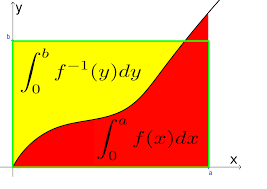
\includegraphics[height=5cm,width=10cm]{young.png}
   \end{minipage}
\end{center}
\end{proof}
We say a pair of numbers $p,q\in [1,\infty]$ are \textbf{exponential conjugated} if 
\begin{align*}
\frac{1}{p}+ \frac{1}{q}=1
\end{align*}
\begin{theorem}
\label{THYi}
\textbf{(Young's inequality for product)} If $a,b \in [0,\infty)$ and $p,q \in (1,\infty)$ is an  exponential conjugated pair, then: 
\begin{align*}
  ab \leq  \frac{a^p}{p} + \frac{b^q}{q}
\end{align*}
Moreover, equality holds if and only if $a^p=b^q$. 
\end{theorem}
\begin{proof}
The proof follows from setting $\phi(x)\triangleq x^{p-1}$ in the \customref{THage}{above geometric estimation}. 
\end{proof}
Fix $1\leq p <\infty$. Let $E\subseteq \R$ be measurable, and define for all $\R$-valued function $f$ measurable on $E$ that 
 \begin{align*}
\norm{f}_p \triangleq \left(\int_E \abso{f}^p  \right)^{\frac{1}{p}}
\end{align*}
and that
\begin{align*}
\norm{f}_\infty \triangleq \inf \set{M\inr_0^+ : f\leq M\text{ a.e. on $E$}}
\end{align*}
Clearly, for all $1\leq p\leq \infty$, the space $L^p(E)$ of $\R$-valued functions  $f$ measurable on $E$ that satisfies  $\norm{f}_p < \infty$ forms a $\R$-vector space. Clearly, the  \textbf{$p$-norms} $\norm{\cdot}_p$ form semi-norms on $L^p(E)$.
\begin{theorem}
\textbf{($L^p$ implies  $L^{p+\epsilon }$ on finite domain)} Let $1\leq p< \infty$ and $E\subseteq \R$. Then: 
\begin{align*}
  \abso{E}<\infty \text{ and } 0\leq N \leq \infty \implies L^{p+N}(E)\subseteq L^p(E)
\end{align*}
\end{theorem}
\begin{proof}
  The $N= \infty$ case is clear. Let $f \in L^{p+N}(E)$. The proof then follows from direct estimation based on splitting: 
\begin{align*}
  E= \set{x \in E: \abso{f(x)}\leq 1}\cup  \set{x \in E: \abso{f(x)}\geq 1}
\end{align*}
\end{proof}
\begin{theorem}
\label{THHi}
\textbf{(Hölder's inequality)} Let  $p,q\in [1,\infty]$ be an exponential conjugated pair, $E\subseteq \R$ be measurable, and $f,g$ be two $\R$-valued functions  measurable on $E$. Then: 
 \begin{align*}
\norm{fg}_1 \leq  \norm{f}_p \norm{g}_q
\end{align*}
If moreover $p>1$, then the equality hold if and only if there exists  $c\inr$ such that $\abso{f}^p=c\abso{g}^q$ a.e. on  $E$. 
\end{theorem}
\begin{proof}
  The proof relies on \emph{normalization}. Before such, we first have to handle the boundary case $p=1$ and $\norm{f}_p=0$.  They are all easy, with the latter an observation that $\norm{f}_p=0 \implies fg=0$ a.e., which follows from definition of Lebesgue integral. \\

We may from now on suppose $1<p<\infty$ and $\norm{f}_p\neq 0 \neq \norm{g}_q$. Define $\widehat{f},\widehat{g}$ by 
\begin{align*}
\widehat{f}\triangleq \frac{f}{\norm{f}_p}\quad \text{ and }\quad \widehat{g}\triangleq \frac{g}{\norm{g}_q} 
\end{align*}
The proof then follows from \customref{THYi}{Young's inequality}:
\begin{align*}
\norm{\widehat{f} \cdot \widehat{g}}_1 \leq \int_E \frac{\abso{\widehat{f}}^p}{p}  + \frac{\abso{\widehat{g}}^q}{q}  = \frac{1}{p}+ \frac{1}{q}=1
\end{align*}
\end{proof}
Let $E \subseteq \R$ be measurable, one may check that $\norm{\cdot}_2$ satisfies  \textbf{parallelogram law} and is thus induced by the obvious inner product: 
\begin{align*}
\langle f,g\rangle \triangleq \int_E f\overline{g}
\end{align*}
Therefore, \customref{THHi}{Hölder’s inequality} become \textbf{Cauchy-Schwarz inequality} of $L^2$-space.  
\section{Fourier series}
Let $L^2(0,P)$ be the space of complex-valued functions $L^2$ on  $(0,P)$. By \customref{THHi}{Hölder’s inequality}, we may well define a semi-$\C$-inner product on $L^2(0,P)$ by: 
\begin{align*}
\langle f,g\rangle \triangleq  \int_0^P f(x)\overline{g(x)}dx \inc
\end{align*}
which induces the $L^2$-norm  $\norm{\cdot}_2$. We then see that $\set{e^{-i 2\pi  n \frac{x}{P}}\quotient \sqrt{P}  : n\inz }$ forms an \textbf{orthonormal system}.



define \textbf{Fourier coefficients} by: 
\begin{align*}
  c_n &\triangleq \langle f, \frac{e^{-i 2\pi  n \frac{x}{P}}}{P}\rangle \\
  \frac{1}{P}\int_0^P f(x) e^{-i  2\pi  n \frac{x}{P}}  dx,\quad \text{ for all } n\inz \\
  a_n&\triangleq  \frac{1}{P}\int_0^P f(x) \cos \left( 2\pi  n \frac{x}{P} \right) dx,\quad \text{ for all }n \inn \cup \set{0}  \\
  b_n&\triangleq  \frac{1}{P}\int_0^P f(x) \sin \left( 2\pi  n \frac{x}{P} \right) dx,\quad \text{ for all }n \inn \cup \set{0}  
\end{align*}

\section{Operator norm}
We define the \textbf{operator norm} of linear $T: \R^n\rightarrow \R^m$ by 
\begin{align*}
\norm{T}_{\operatorname{op}}\triangleq \sup_{\textbf{x}\neq 0} \frac{\abso{T\textbf{x}}}{\abso{\textbf{x}}}=  \max_{\textbf{x}=1} \abso{T\textbf{x}}
\end{align*}
One may check that this forms a norm on the real vector space of linear mappings from $\R^n$ to  $\R^m$. \textbf{Singular Value Decomposition Theorem} said that for each linear $T :\R^n\rightarrow \R^m$, there exists some orthonormal basis $\set{\textbf{v}_1,\dots ,\textbf{v}_n}$ such that $\set{T(\textbf{v}_1),\dots ,T(\textbf{v}_m)}- \set{\textbf{0}}$ is orthogonal. We call $\abso{T(\textbf{v}_1)},\dots ,\abso{T(\textbf{v}_n)}$ the \textbf{singular values} of $T$. 
\begin{theorem}
\textbf{(Operator norm is the largest singular value)} The operator norm of linear $T:\R^n\rightarrow \R^m$ is exactly the largest singular value of $T$. 
\end{theorem}
\begin{proof}

\end{proof}
\begin{theorem}
\textbf{(Equivalence of norms on $\R^n$)}
\end{theorem}
Now use the fact that determinant is continuous to conclude that collection of invertible function in $\operatorname{End}_{\text{linear}}(\R^n)$ is open. 
\begin{theorem}
\label{THIic}
\textbf{(Inversion is Continuous)} Let $\Omega$ be the space of invertible linear functions from $\R^n$ to itself. The mapping $\Omega\rightarrow \Omega,A \mapsto  A^{-1}$ is continuous. 
\end{theorem}
\begin{proof}
Stick to the one in General Analysis. 
\end{proof}
\begin{theorem}
\label{DT}
\textbf{(Differentiability Theorem)} Suppose  $\alpha =\set{e_1,\dots ,e_n}$ is an orthonormal basis of $\R^n$, and $\beta =\set{q_1,\dots ,q_m}$ is an orthonormal basis of  $\R^m$. Suppose  $f$ maps an open set $E\subseteq\R^n$ to $\R^m$.  Then  
\begin{align*}
f\text{ is continuously differentiable on $E$ }\iff \partial_if_j\text{ exists and is continuous on $E$ for all $i,j$ }
\end{align*}
\end{theorem}
\begin{proof}
$(\longrightarrow)$\\

Fix $i,j$. Because $f$ is differentiable on $E$, we know  $\partial_i f_j$ exists on $E$ by \myref{Theorem}{DiJ}. Fix $x \in E$. We only have to show 
\begin{align*}
  \vi{\partial_i f_j\text{ is continuous at $x$ }}
\end{align*}
Fix $\epsilon $. We wish 
\begin{align*}
\vi{\text{ to find }\delta\text{ such that } \abso{\partial_i f_j(y)-\partial_i f_j(x)}\leq \epsilon \text{ for all $\abso{y-x}<\delta$ }}
\end{align*}
Because $f$ is continuously differentaible at $x$, we know there exists  $\delta$ such that 
\begin{align*}
\norm{df_y-df_x}_\text{op}< \epsilon \text{ for all $\abso{y-x}\leq \delta$ }
\end{align*}
We claim 
\begin{align*}
\vi{\text{ such $\delta$ suffices }}
\end{align*}
By the \customref{DiJ}{the matrix representation}, we know
\begin{align*}
\partial_i f_j(y)-\partial_i f_j(x)=(df_y-df_x)e_i \cdot q_j
\end{align*}
Then by Cauchy-Inequality, we have 
\begin{align*}
  \abso{\partial_i f_j(y)-\partial_if_j(x)}&\leq \abso{(df_y-df_x)e_i}\\
  &\leq \norm{df_y-df_x}_\text{op}<\epsilon \vdone
\end{align*}

$(\longleftarrow)$\\

We first show 
\begin{align*}
\vi{f\text{ is differentiable on $E$ }}
\end{align*}
We first prove 
\begin{align*}
\olive{\forall j\in \set{1,\dots, m}, f_j:\R^n\rightarrow \R\text{ is differentiable on $E$ }\implies f\text{ is differentiable on $E$ }}
\end{align*}
Fix $x\in E$. We wish to prove 
\begin{align*}
\olive{\text{ $f$ is differentiable at $x$ }}
\end{align*}
Define $A:E\rightarrow \R^m$ by 
\begin{align*}
A(h)\triangleq \sum_{j=1}^m  (df_j)_x (h)q_j
\end{align*}
We claim 
\begin{align*}
\olive{A\text{ suffices to be the $df_x$ }}
\end{align*}
Using the fact $q_j$ are orthonormal, we have
\begin{align*}
f(x+h)-f(x)-A(h)=\sum_{j=1}^m \big(f_j(x+h)-f_j(x)-(df_j)_x(h)  \big)q_j
\end{align*}
This give us 
\begin{align*}
\lim_{h\to 0} \frac{\abso{f(x+h)-f(x)-A(h)}}{\abso{h}}&=\lim_{h\to 0} \frac{\abso{\sum_{j=1}^m \big(f_j(x+h)-f_j(x)-(df_j)_x (h) \big)q_j}}{\abso{h}}\\
&\leq \lim_{h\to 0} \frac{\sum_{j=1}^m \abso{f_j(x+h)-f_j(x)-(df_j)_x(h)}}{\abso{h}}=0 \odone
\end{align*}
Fix $j \in \set{1,\dots ,m}$. We can now reduce the problem into 
\begin{align*}
  \vi{f_j:\R^n\rightarrow \R\text{ is differentiable on $E$ }}
\end{align*}
Fix $x \in E$. We wish to prove 
\begin{align*}
\vi{f_j\text{ is differentiable at $x$ }}
\end{align*}
Express $h=\sum_{i=1}^n h_ie_i$. Define $B:E\rightarrow \R$ by
\begin{align*}
B(h)=\sum_{i=1}^n \partial_i f_j(x)h_i
\end{align*}
We claim 
\begin{align*}
\vi{B\text{ suffices to be $(df_j)_x$ }}
\end{align*}
By continuity of each $\partial_i f_j$ on $E$, we can let  $\delta$ satisfy 
\begin{align*}
\abso{\partial_i f_j(y)-\partial_i f_j(x)}<  \frac{\epsilon }{n}  \text{ for all $y\in B_\delta(x)$  }
\end{align*}
We claim 
\begin{align*}
  \vi{\frac{\abso{f_j(y)-f_j(x)-B(y-x)}}{\abso{y-x}}\leq \epsilon \text{ for all }y \in B_\delta (x)}
\end{align*}
Express $y-x=\sum_{k=1}^n h_ke_k$. Define $v_0,\dots,v_n\inr^n$ by
\begin{align*}
v_0\triangleq 0\text{ and }v_k\triangleq \sum_{i=1}^k h_ie_i\text{ for all $k\in \set{1,\dots ,n}$ }
\end{align*}
Now observe
\begin{align*}
\frac{\abso{f_j(y)-f_j(x)-B(y-x)}}{\abso{y-x}}&=\frac{\abso{f_j(x+v_n)-f_j(x)-B(\sum_{k=1}^n h_ke_k)}}{\abso{y-x}}\\
&=\frac{\abso{\big(\sum_{k=1}^nf_j(x+v_k)-f_j(x+v_{k-1}) \big)- \sum_{k=1}^n \partial_k f_j(x)h_k   }}{\abso{y-x}}\\
&=\frac{\abso{\sum_{k=1}^n f_j(x+v_k)-f_j(x+v_{k-1})-\partial_k f_j(x)h_k}}{\abso{y-x}}\\
&=\frac{\abso{\sum_{k=1}^n f_j(x+v_{k-1}+h_ke_k)-f_j(x+v_{k-1})-\partial_k f_j(x)h_k}}{\abso{y-x}}\\
(\text{ For some $e_k\in (0,1)$ by \customref{MVT}{MVT}})\hspace{0.5cm}&=\frac{\abso{\sum_{k=1}^n \partial_k f_j(x+v_{k-1}+t_ke_k)h_k-\partial_k f_j(x)h_k}}{\abso{y-x}}\\
&\leq \frac{\sum_{k=1}^n \abso{\big(\partial_k f_j(x+v_{k-1}+t_ke_k)-\partial_k f_j(x) \big)h_k}}{\abso{y-x}}\\
&< \frac{\sum_{k=1}^n \frac{\epsilon }{n} \abso{h_k}}{\abso{y-x}}\leq \epsilon \vdone
\end{align*}
We now prove
\begin{align*}
\blue{f\text{ is continuously differentiable on $E$ }}
\end{align*}
Fix $\epsilon $ and $x\in E$. We are required 
\begin{align*}
\blue{\text{ to find $\delta$ such that $\norm{df_y-df_x}_\text{op}\leq \epsilon $ for all $y\in B_\delta (x)$ }}
\end{align*}
Note that one can define a norm $\norm{\cdot}_F$ called "Forbenius Norm" on $BL(\R^n,\R^n)$ by 
\begin{align*}
\norm{A}_F\triangleq \sqrt{\sum_{i=1}^n \sum_{j=1}^n a_{i,j}^2}  \text{ where }[A]_\alpha ^\beta = \begin{bmatrix}
  a_{1,1}& \cdots & a_{n,1}\\
  \vdots & \ddots & \vdots \\
  a_{1,n} & \cdots & a_{n,n}  
\end{bmatrix}
\end{align*}
Because \customref{ANoF}{all norms on finite-dimensional real vector spaces are equivalent}, we know there exists $M$ such that for all $x\in E$, we have 
\begin{align*}
\norm{df_x}_\text{op}\leq  M\norm{df_x}_F
\end{align*}
Because the partial derivatives are all continuous by definition, we can let $\delta$ satisfy 
\begin{align*}
  \big(\partial_i f_j(x+h)\big)^2-\big(\partial_i f_j(x)\big)^2< \frac{\epsilon^2 }{M^2n^2}\text{ for all $h \in B_\delta (0)$ }
\end{align*}
We claim 
\begin{align*}
\blue{\text{ such }\delta\text{ suffices }}
\end{align*}
Let $\abso{y-x}<\delta$. We see 
\begin{align*}
\norm{df_y-df_x}_\text{op}\leq M\norm{df_y -df_x}_F< M \sqrt{\sum_{i=1}^n \sum_{j=1}^n\frac{\epsilon^2 }{M^2n^2}}=\epsilon \bdone
\end{align*}












\end{proof}
\section{Inverse function theorem}
Let $X$ be a metric space. A \textbf{contraction} $f:X\rightarrow X$ is a $K$-Lipschitz function such that $K<1$.  
\begin{example}
Let $X\triangleq \R$. $f(x)\triangleq \frac{x}{2}$ is a $\frac{1}{2}$-contraction, and $g(x)\triangleq x$ for no $r\in [0,1)$ is a $r$-contraction.  
\end{example}
\begin{theorem}
\textbf{(Banach's fixed point theorem)}  Let $X$ be a metric space. Let $f:X\rightarrow X$ be a contraction. Then $f$ admits at most one fixed point. Let $f^n:X\rightarrow X$ denote: 
\begin{align*}
\overbrace{f\circ \cdots \circ f}^{n\text{ copies }}:X\rightarrow X
\end{align*}
If $X$ is moreover complete, then for all $x \in X$, the sequence $\set{f^n(x)}\subseteq X$ converges, with limit being a (the unique) fixed point of $f$. 
\end{theorem}
\begin{proof}
It is easy to see from the definition that a contraction can only have at most one fixed point from the definition. Let $X$ be complete and $x \in X$. Because $f$ as a Lipschitz function is continuous, we know that if $\set{f^n(x)}\subseteq X$  converges, then its limit is a (the unique) fixed point of $f$: 
\begin{align*}
f \left(\lim_{n\to \infty}f^n(x)\right)=\lim_{n\to \infty}f^{n+1}(x)=\lim_{n\to \infty}f^n(x)
\end{align*}
It remains to prove  $\set{f^n(x)}\subseteq X$ converges. Because $X$ is complete, we only have to prove  $\set{f^n(x)}\subseteq X$ is Cauchy. Fix $\epsilon $. Because $0\leq K<1$, we may find $N$ large enough so that $\frac{K^N}{1-K}d(x,f(x))\leq \epsilon $. We claim that for all $n\geq N$ and $k\inn$, we have: 
\begin{align}
\label{EQdfnk}
d(f^n(x),f^{n+k}(x))\leq \epsilon,\quad \text{ as desired. }
\end{align}
We now prove \myref{inequality}{EQdfnk}. We first note that, using induction on $k$ and triangle inequality, we have: 
\begin{align*}
d(x,f^k(x))= \sum_{j=0}^{k-1}K^j d(x,f^k(x)) \leq \frac{1}{1-K} d(x,f^k(x))
\end{align*}
This then implies 
\begin{align*}
d(f^n(x),f^{n+k}(x))\leq K^n d(x,f^k(x))  \leq \frac{K^n}{1-K} d(x,f(x))\leq \epsilon 
\end{align*}
as desired.
\end{proof}
\begin{theorem}
\label{THpift}
\textbf{(Pointwise inverse function theorem)} Let $U$ be some neighborhood of  $\textbf{a}\in \R^n$. If differentiable $\textbf{f}:U\rightarrow \R^n$ is $C^1$ at $\textbf{a}$ and has full rank Jacobian at $\textbf{a}$, then: 
\begin{enumerate}[label=(\roman*)]
  \item  $\textbf{f}$ maps some $B_\delta (\textbf{a})\subseteq U$ injectively to some open subset of $\R^n$. 
  \item Moreover, the local inverse of $\textbf{f}$ is differentiable at $\textbf{f}(\textbf{a})$. 
\end{enumerate}
\end{theorem} 
\begin{proof}

\end{proof}
\begin{corollary}
\label{THift}
\textbf{(Inverse function theorem)} Let $U$ be some neighborhood of $\textbf{a}$. If $C^1$ function $\textbf{f}:U\rightarrow \R^n$ has full rank Jacobian at $\textbf{a}$, then $\textbf{f}$ forms a $C^1$-diffeomorphism between some neighborhood  $W\ni \textbf{a}$ contained by $U$, and  $\textbf{f}(W)$.      
\end{corollary}
\begin{proof}
Because $\operatorname{GL}_n(\R)\subseteq \operatorname{M}_n(\R)$ is open and $\textbf{f}$ is $C^1$, we know there exists some neighborhood $U'\ni \textbf{a}$ contained by $U$ such that  $\textbf{f}$ has full rank Jacobian everywhere in $U'$. Applying \customref{THpift}{pointwise inverse function theorem} for every point in $U'$, we get an injective  $C^1$-function $\textbf{f}:W \rightarrow \R^n$ with differentiable inverse. To see $(\textbf{f})^{-1}:\textbf{f}(W)\rightarrow W$ is also $C^1$, just observe:  
\begin{align*}
\textbf{y}\mapsto d\textbf{f}^{-1}|_\textbf{y} =   \left(\textbf{x} \mapsto (d\textbf{f}|_\textbf{x})^{-1} \right) \circ  \left(\textbf{y}\mapsto \textbf{f}^{-1}(\textbf{y}) \right)
\end{align*}
and recall that \customref{THIic}{$GL_n(\R)\rightarrow GL_n(\R),A \mapsto A^{-1}$ is continuous}. 
\end{proof}
\section{Implicit function theorem}
\begin{theorem}
\label{THipft}
\textbf{(Implicit function theorem)} Let $W \subseteq \R^n \times \R^m$ be open and $(\textbf{a},\textbf{b}) \in W$. Let $\textbf{f}:W\rightarrow \R^n$ be a $C^1$  function such that the matrix: 
\begin{align*}
\begin{pmatrix} 
  \frac{\partial f_1}{\partial x_1} \Big  |_{(\textbf{a},\textbf{b})} & \cdots & \frac{\partial f_1}{\partial x_n} \Big |_{(\textbf{a},\textbf{b})}  \\
  \vdots & \ddots & \vdots \\
  \frac{\partial f_n}{\partial x_1} \Big|_{(\textbf{a},\textbf{b})} & \cdots & \frac{\partial f_n}{\partial x_n} \Big  |_{(\textbf{a},\textbf{b})} 
\end{pmatrix}
\end{align*}
is invertible. Then, there exists a pair of neighborhoods $U \ni (\textbf{a},\textbf{b})$ and $V \ni \textbf{b}$ such that: For all  $\textbf{y} \in V$ there exists a unique $\textbf{x} \inr^n$ that satisfies both  $(\textbf{x},\textbf{y})\in U$ and $\textbf{f}(\textbf{x},\textbf{y})=\textbf{f}(\textbf{a},\textbf{b})$. Moreover, if we define $\textbf{g}:V \rightarrow \R^n$ by setting 
\begin{align*}
\textbf{f}(\textbf{g}(\textbf{y}), \textbf{y}) = \textbf{f}(\textbf{a},\textbf{b}),\quad \text{ for all }\textbf{y} \in V
\end{align*}
then $\textbf{g}$ will be $C^1$ and clearly make $\textbf{g}(\textbf{b})=\textbf{a}$. 


\end{theorem}
\begin{proof}
Define $\textbf{F}: W \rightarrow \R^n \times \R^m$ by 
\begin{align*}
\textbf{F}(\textbf{x},\textbf{y})\triangleq \left(\textbf{f}(\textbf{x},\textbf{y}),\textbf{y} \right)
\end{align*}
By \customref{DT}{differentiability theorem}, $\textbf{F}$ is $C^1$. Clearly, the Jacobian of $\textbf{F}$ at $\left(\textbf{a},\textbf{b}\right)$ is full rank.  We may now apply \customref{THift}{inverse function theorem} to find some smaller neighborhood $U \subseteq W$ of $\left(\textbf{a},\textbf{b} \right)$ such that: 
\begin{enumerate}[label=(\Roman*)]
  \item $\textbf{F}$ is injective on $U$.  
  \item $\textbf{F}(U)\subseteq \R^n \times \R^m$ is open.
  \item $\textbf{F}$ has full rank Jacobian everywhere in $U$.  
  \item The local inverse $\textbf{F}^{-1}: \textbf{F}(U)\rightarrow U$ is $C^1$.   
\end{enumerate}
Because $\textbf{F}(U)$ is open, we know 
\begin{align*}
V \triangleq \set{\textbf{y} \inr^m: (\textbf{f}(\textbf{a},\textbf{b}),\textbf{y}) \in \textbf{F}(U)}\text{ is open }
\end{align*}
We claim such $U\ni (\textbf{a},\textbf{b})$ and  $V\ni \textbf{b}$ suffices. Fix $\textbf{y}\in V$. We are required to show the existence and uniqueness of $\textbf{x}\inr^n$ that satisfies both $(\textbf{x},\textbf{y})\in U$ and $\textbf{f}(\textbf{x},\textbf{y})=\textbf{f}(\textbf{a},\textbf{b})$. \\

By definition of $V$, we know  $\left(\textbf{f}(\textbf{a},\textbf{b}), \textbf{y} \right)\in \textbf{F}(U)$. Therefore, there exist $\textbf{z}=(\textbf{z}_1,\textbf{z}_2)\in U$ such that $\textbf{F}(\textbf{z})=\left(\textbf{f}(\textbf{a},\textbf{b}),\textbf{y} \right)$. By definition of $\textbf{F}$, $\textbf{z}_1$ is the $\textbf{x}$ we are looking for. Moreover, because $\textbf{F}$ is injective on $U$, we know $\textbf{z}_1$ is the only option. We have shown the existence and uniqueness of $\textbf{x}$. It remains to prove that $\textbf{g}$ is $C^1$, which follows from \customref{DT}{differentiability theorem} and that $\left(\textbf{g}(\textbf{y}),\textbf{y} \right)=\textbf{F}^{-1}\left(\textbf{f}(\textbf{a},\textbf{b}),\textbf{y}\right)$ for all $\textbf{y}\in V$. 
\end{proof}
Note that $\textbf{g}$ clearly satisfies:
    \begin{align*}
\begin{pmatrix} 
  \frac{\partial g_1}{\partial y_1} \Big|_{\textbf{y}} & \cdots & \frac{\partial g_1}{\partial y_m} \Big|_{\textbf{y}} \\
  \vdots & \ddots & \vdots \\
  \frac{\partial g_n}{\partial y_1} \Big|_{\textbf{y}} & \cdots & \frac{\partial g_n}{\partial y_m} \Big|_{\textbf{y}}
\end{pmatrix} = -  
\begin{pmatrix} 
  \frac{\partial f_1}{\partial x_1} \Big  |_{(\textbf{g}(\textbf{y}),\textbf{y})} & \cdots & \frac{\partial f_1}{\partial x_n} \Big |_{(\textbf{g}(\textbf{y}),\textbf{y})}  \\
  \vdots & \ddots & \vdots \\
  \frac{\partial f_n}{\partial x_1} \Big|_{(\textbf{g}(\textbf{y}),\textbf{y})} & \cdots & \frac{\partial f_n}{\partial x_n} \Big  |_{(\textbf{g}(\textbf{y}),\textbf{y})} 
\end{pmatrix}^{-1} \cdot \begin{pmatrix} 
  \frac{\partial f_1}{\partial y_1} \Big|_{(\textbf{g}(\textbf{y}),\textbf{y})} & \cdots & \frac{\partial f_1}{\partial y_m}  \Big |_{(\textbf{g(\textbf{y})},\textbf{y})} \\
  \vdots & \ddots & \vdots \\
  \frac{\partial f_n}{\partial y_1} \Big|_{(\textbf{g}(\textbf{y}),\textbf{y})} & \cdots & \frac{\partial f_n}{\partial y_m}  \Big |_{(\textbf{g}(\textbf{y}),\textbf{y})} 
\end{pmatrix}
\end{align*}
for all $\textbf{y} \in V$, which in particular \customref{DT}{manifest the fact that $\textbf{g}$ is $C^1$}. 
\section{Legendre type formula}
\section{Miscellaneous}
\begin{theorem}
\label{THSa}
\textbf{(Stirling's approximation)} 
\begin{align*}
n!\sim \sqrt{2\pi n} \left(\frac{n}{e} \right)^n  ,\quad \text{ as }n\rightarrow \infty
\end{align*}
\end{theorem}
\begin{theorem}
\label{THLmt}
\textbf{(Lagrange multiplier theorem)} Let $V \subseteq \R^n$ be open , $f,g_1,\dots ,g_m \in C^1(V)$ with $m\leq n$, and $\textbf{y}\in V$. If: 
\begin{enumerate}[label=(\roman*)]
  \item $\textbf{y}$ is a local extremum of $f$ subject to the constraints $g_1(\textbf{x})=\cdots = g_m(\textbf{x})=0$. 
  \item 
    \begin{align*}
    \operatorname{rank} \begin{pmatrix} 
      \frac{\partial g_1}{\partial x_1} (\textbf{x}) & \cdots & \frac{\partial g_1}{\partial x_n}(\textbf{x}) \\
      \vdots & \ddots & \vdots \\
      \frac{\partial g_m}{\partial x_1}(\textbf{x}) & \cdots & \frac{\partial g_m}{\partial x_n} (\textbf{x})
    \end{pmatrix} = m
    \end{align*}
\end{enumerate}
then there exists a unique $(\ld_1,\dots ,\ld _m)\inr^m$  such that 
\begin{align*}
\nabla f (\textbf{y})= \sum_{i=1}^m \ld_i \nabla g_i (\textbf{y})
\end{align*}
\end{theorem}
\begin{theorem}
\label{THdivt}
\textbf{(Divergence theorem)}  Let $M \subseteq \R^3$ be compact with piecewise smooth boundary and $\textbf{F}:M\rightarrow \R^3$ be $C^1$. Then:  
\begin{align*}
\int_{\partial M} \textbf{F} \cdot \textbf{n} dA = \int_{M} \nabla \cdot \textbf{F} dV 
\end{align*}
\end{theorem}
\begin{theorem}
\label{THGt}
\textbf{(Green's theorem)} Let $C\subseteq \R^2$ be a positively oriented, piecewise smooth, and smooth curve. Let $D\subseteq \R^2$ be the region bounded by $C$. If  $L,M \in C^1(D)$, then 
\begin{align*}
\int_C Ldx+M dy= \int_D \begin{vmatrix} 
  \frac{\partial }{\partial x} & \frac{\partial }{\partial y} \\
  L & M 
\end{vmatrix} dA 
\end{align*}
\end{theorem}
\begin{theorem}
\label{THmTt}
\textbf{(Multivariable Taylor's theorem)} Let  $U$ be a neighborhood of $\textbf{a}\inr^n$, and let $f\in C^k(U)$. Consider the   multi-index notation  
\begin{align*}
  \abso{\alpha }\triangleq  \alpha_1 + \cdots + \alpha _n,\quad  \alpha ! \triangleq \alpha_1! \cdots \alpha_n!,\quad  \textbf{x}^{\alpha }\triangleq  x_1^{\alpha _1}\cdots x_n^{\alpha _n}   
\end{align*}
We have: 
\begin{align*}
f(\textbf{x})= f(\textbf{a})+\sum_{1\leq \abso{\alpha }\leq k} \frac{1}{\alpha !}\cdot  \frac{\partial^k f}{\partial x_1^{\alpha _1} \cdots \partial x_n^{\alpha _n}} \bigg|_{\textbf{a}} (\textbf{x}-\textbf{a})^{\alpha } + o( \abso{\textbf{x}-\textbf{a}}^k)
\end{align*}
\end{theorem}
\section{Legendre formula}
Let $f$ be a $\R$-valued  $C^1$ function near  $\textbf{0}\inr^n$. Suppose $\operatorname{Hess}f$ is invertible at $\textbf{0}$. Therefore, there exists some neighborhood $U$ of $\textbf{0}\inr^n$ on which $\nabla f$ forms a $C^1$-diffeomorphism onto $V \subseteq \R^n$. Let $\textbf{G}:V \rightarrow U$ be the inverse function of $\nabla f$. We hope that there exists some $h:V \rightarrow \R$ such that $\nabla h=\textbf{G}$. Such is feasible. Let 
\begin{align*}
h (\textbf{y})\triangleq \textbf{G}(\textbf{y}) \cdot \textbf{y} - f\circ \textbf{G}(\textbf{y})
\end{align*}
Compute 
\begin{align*}
\frac{\partial h}{\partial y_1}= G_1 + \frac{\partial G_1}{\partial y_1} \cdot y_1 + \sum_{i=2}^n \frac{\partial G_i}{\partial y_i} y_i - \sum_{i=1}^n \frac{\partial f}{\partial x_i} \cdot \frac{\partial G_i}{\partial y_i} = G_1
\end{align*}
\section{weighted $p$-norm}
\begin{theorem}
\textbf{(weighted $\infty$-norm)} Let $v_1,\dots ,v_n \geq 0$ and $w_1,\dots ,w_n >0$ satisfies $\sum w_i=1$. We have: 
\begin{align*}
\lim_{p\to \infty} \left(\sum w_i v_i^p   \right)^{\frac{1}{p}}= \max v_i
\end{align*}
\end{theorem}
\begin{proof}
Let $v_1\leq \cdots \leq v_n$. Clearly, 
\begin{align*}
  \left(\sum w_i v_i^p \right)^{\frac{1}{p}} \leq \left( v_n^p \right)^{\frac{1}{p}}= v_n 
\end{align*}
and clearly, 
\begin{align*}
 \left( \sum w_i v_i^{p} \right)^{\frac{1}{p}} \geq (w_nv_n^p)^{\frac{1}{p}} \rightarrow v_n,\quad \text{ as }p\rightarrow  \infty
\end{align*}
\end{proof}
Note that this also implies that 
\begin{align*}
  (v_1^p+\cdots + v_n^p)^{\frac{1}{p}}\rightarrow \max v_i
\end{align*}
\begin{theorem}
\textbf{(weighted $0$-norm)}  Let $v_1,\dots ,v_n \geq 0$ and $w_1,\dots ,w_n >0$ satisfies $\sum w_i=1$. We have: 
\begin{align*}
\lim_{p\to 0} \left(\sum w_i v_i^p   \right)^{\frac{1}{p}}= \prod v_i^{w_i}
\end{align*}
\end{theorem}
\begin{proof}
Compute 
\begin{align*}
  \left( \sum w_iv_i^p \right)^{\frac{1}{p}}= \exp \left(\frac{\ln \left(\sum w_iv_i^p\right)}{p}  \right)
\end{align*}
By  \customref{L'Hospital Rule}{L'Hospital Rule}, we have
\begin{align*}
\lim_{p\to 0} \frac{\ln \left(\sum w_iv_i^p \right)}{p} = \lim_{p\to 0}\frac{ \ln (v_i)w_iv_i^p}{\sum w_iv_i^p}= \sum  \ln (v_i)w_i
\end{align*}

\end{proof}
\section{Continuous Convergent}
Let $M,N$ be a metric space and  $f_n:M \rightarrow N$ be a pointwise convergent sequence that makes all convergent sequence $\set{x_n}\subseteq M$ satisfies:
\begin{align*}
\lim_{n\to \infty} f_n(x_n)= f(\lim_{n\to \infty}x_n)
\end{align*}
Let $x_k\rightarrow x$. To see $f(x_k)\rightarrow f(x)$, consider the subsequence $n_k$ that makes 
\begin{align*}
d\left(f_{n_k}(x_k),f(x_k)\right)\leq \frac{\epsilon}{2}
\end{align*}
Noting that 
\begin{align*}
  \overbrace{x_1,\dots ,x_1}^{n_1\text{ copies }},\overbrace{x_2,\dots , x_2}^{n_2-n_1\text{ copies }},\dots ,
\end{align*}
converges to $x$, we see 
 \begin{align*}
d\left(f(x_k),f(x)\right) \leq d\left( f(x_k), f_{n_k}(x_k)\right) + d\left( f_{n_k}(x_k),f(x) \right) 
\end{align*}
has limit superior $\frac{\epsilon}{2}$. Note that $f_n$ need not be continuous, and the convergence need not be uniform. 
\begin{example}
Let $M\triangleq [0,2)$
\begin{align*}
f_n\triangleq  \frac{1}{1+n(2-x_n)}
\end{align*} 
\end{example}
However, clearly the convergence is uniform if we require $M$ to be compact. 




\section{Function spaces exercises}
\begin{question}{}{}
Let $f:[0,1]\rightarrow [0,1]$ satisfies 
\begin{enumerate}[label=(\roman*)]
  \item $f$ is  $C^1$.  
  \item $f(0)=0=f(1)$. 
  \item $f'$ is decreasing. 
\end{enumerate}
Show that the arc-length of the graph of $f$ does not exceed $3$. 
\end{question}
\begin{proof}
Because for all $t \in(0,1)$, we have 
\begin{align*}
 \left( 1+ \abso{f'(t)} \right)^2 \geq 1 + (f'(t))^2
\end{align*}
we know 
\begin{align*}
\int_0^1 \sqrt{1+ (f'(t))^2 } dt \leq \int_0^1  \left( 1 + \abso{f'(t)} \right) dt  =  1+ \int_0^1 \abso{f'(t)}dt
\end{align*}
If $f'(0)\leq 0$, then $f$ is constant zero so there is nothing to prove. We from now on suppose  $f'(0)>0$.\\ 

By EVT, we know $f$ attains maximum at some point. Because $f$ is $C^1$ we know at that point the derivative is  $0$. This implies that the maximum is unique. Let that point be $x$. We now see 
\begin{align*}
\int_0^1 \abso{f'(t)}dt = \int_0^x f'(t)dt + \int_x^1 -f'(t)dt \leq 2
\end{align*}
\end{proof}
\begin{question}{}{}
Let $f$ be a  $C^2$ function on the real line with 
 \begin{align*}
A\triangleq \sup \abso{f} \inr\text{ and }B\triangleq \sup \abso{f''} \inr 
\end{align*}
Show that 
\begin{align*}
\sup\abso{f'} \leq 2\sqrt{AB} 
\end{align*}
\end{question}
\begin{proof}
Assume for a contradiction that $f'(x)> 2\sqrt{AB}$. It then follows from $\sup \abso{f''}=B$ that 
\begin{align*}
\int_{x- 2\sqrt{\frac{A}{B}}}^{x+ 2 \sqrt{\frac{A}{B}} } f'(t) dt \geq 4A 
\end{align*}
which implies that either $f(x+ 2 \sqrt{\frac{A}{B}} )$ or $f(x- 2 \sqrt{\frac{A}{B}} )$ lies outside of $[-A,A]$. 
\end{proof}
\begin{question}{}{}
Let $f$ be continuous on $\R$ and let 
 \begin{align*}
f_n(x)\triangleq \frac{1}{n}\sum_{k=0}^{n-1} f\left(x+\frac{k}{n} \right)
\end{align*}
Prove that $f_n$ converges compactly. 
\end{question}
\begin{proof}
Observe 
\begin{align*}
\int_{x}^{x+1} f(t)dt - f_n(x)= \sum_{k=0}^{n-1} \int_{x+\frac{k}{n}}^{x+ \frac{k+1}{n}} \left(f(t)- f(x+\frac{k}{n}) \right) dt 
\end{align*}
\end{proof}
\begin{question}{}{}
Let $f:[0,1]\rightarrow \R$ be $C^1$ with  $\sup \abso{f'} = M \inr$. Prove that for all $n$, we have 
\begin{align*}
\abso{\frac{1}{n}\sum_{k=0}^{n-1}f\left(\frac{k}{n} \right) - \int_0^1 f(x)dx} \leq \frac{M}{2n}
\end{align*}
\end{question}
\begin{proof}
Observe 
\begin{align*}
\frac{1}{n} \sum_{k=0}^{n-1}f\left(\frac{k}{n} \right)- \int_0^1 f(x)dx = \sum_{k=0}^{n-1}\int_{\frac{k}{n}}^{\frac{k+1}{n}} \left(f\left(\frac{k}{n} \right) - f(x) \right)dx
\end{align*}
The integrands clearly are all smaller than $\frac{M}{2n^2}$. 
\end{proof}
\begin{question}{}{}
Suppose that $f_n \in C^0$ and for each $x \in [a,b]$, we have 
\begin{align*}
f_n(x)\searrow 0
\end{align*}
Show that $f_n$ are equicontinuous. 
\end{question}
\begin{proof}
  By \customref{THDt}{Dini's theorem}. Fix $\epsilon $. Because the convergence is uniform, there exists some $N$ such that  $f_n(x)\leq \epsilon $ for all $n\geq N$. Because $\set{f_1,\dots ,f_{N-1}}$ are all uniform continuous, we now see that the minimum of $\set{\delta_1,\dots ,\delta_{N-1}}$ suffices. 
\end{proof}
\begin{question}{}{}
Let $E$ be the space of all $1$-Lipschitz function $u:[0,1]\rightarrow \R$  such that $u(0)=0$. Define $\pfi  : E \rightarrow \R$ by 
\begin{align*}
  \pfi(u)\triangleq \int_0^1 \left(u(x)^2 - u(x) \right)dx
\end{align*}
Show that $\pfi $ attains maximum at some $u$, 
\end{question}
\begin{proof}
The fact that $E$ is compact in the uniform norm topology  follows at once from \customref{THaat}{Arezela-Ascoli theorem}. It then remains to show $\pfi $ is continuous. Observe 
\begin{align*}
  \abso{\pfi  (u)-\pfi  (v)}&\leq   \abso{\int_0^1 u^2-v^2 -u +v}  \\
  & \leq  \int_0^1 \abso{u-v} + \abso{u-v} \cdot \abso{u+v}     \\
  & \leq  \int_0^1 \abso{u-v} \left(1 + \abso{u}+ \abso{v} \right) \leq 3 \norm{u-v}_{\infty} 
\end{align*}
\end{proof}
\begin{question}{}{}
Let $\set{a_n}$ be a sequence of nonzero real numbers. Prove that 
\begin{align*}
f_n(x)= \frac{\sin (a_nx)}{a_n} + \cos (x+ a_n)
\end{align*}
has a subsequence converging to a continuous function. 
\end{question}
\begin{proof}
We are looking for a subsequence that converge compactly. Fix $R\inn$. Because $\sin (a_nx) \leq a_nx$, we know $f_n$ is uniformly bounded on  $[-R,R]$ by $R+1$. Clearly $f_n$ are uniformly equicontinuous on $\R$. Applying \customref{THaat}{Arezela-Ascoli theorem} onto $\set{f_n}$ on $[-1,1]$, we get a subsequence $\set{f_n^{(1)}}$ that uniformly converge on $[-1,1]$. Applying   \customref{THaat}{Arezela-Ascoli theorem} onto $\set{f_n^{(1)}}$ on $[-2,2]$, we get a subsequence $\set{f_n^{(2)}} \subseteq \set{f_n^{(1)}}$ that uniformly converge on $[-2,2]$. Then taking the diagonal $\set{f^{(n)}_n}$, we see it uniformly converges on $[-R,R]$ for all $R$, as its tails lies in  $\set{f^{(R)}_n}$ for all $R$.  
\end{proof}
\begin{question}{}{}
Suppose the limits of $f:[a,b]\rightarrow \R$ from left to right exists at all $x\in [a,b]$. Show that $f$ is Riemann integrable. 
\end{question}
\begin{proof}
Fix $\epsilon $. By premise, for each $x \in (a,b)$, we may find $\delta_{x,-},\delta_{x,+}$ such that 
\begin{align*}
\operatorname{osc}(f, (x-\delta_{x,-},x)) \leq \frac{\epsilon }{b-a}\quad  \text{ and }\quad \operatorname{osc}(f,(x,x+\delta_{x,+})) \leq \frac{\epsilon}{b-a}
\end{align*}
We may also find $\delta_{a,+},\delta_{b,-}$ that makes 
\begin{align*}
  \operatorname{osc}(f,[a,a+\delta_{a,+}))\leq \frac{\epsilon}{b-a} \quad \text{ and }\quad \operatorname{osc}(f,(b-\delta_{b,-},b]) \leq \frac{\epsilon}{b-a}
\end{align*}
Consider a finite subcover of  $[a+\delta_{a,+},b-\delta_{b,-}]$ of the intervals. The endpoints of these interval clearly forms a sufficing partition.  
\end{proof}
\begin{question}{}{}
Suppose that $f \in C^3[-1,1]$. Prove that the series 
\begin{align*}
\sum_{n=0}^{\infty} \left( n\left(f\left(\frac{1}{n} \right)- f\left(\frac{-1}{n} \right) \right) - 2f'(0)\right)
\end{align*}
converges.  
\end{question}
\begin{question}{}{}
Let $f:[0,1]\rightarrow \R$ be $C^1$ with  $f(0)=0$. Prove that 
\begin{align*}
\norm{f}^2_{\infty}\leq \int_0^1 \left(f'(x) \right)^2dx
\end{align*}
\end{question}
\begin{proof}
We are required to prove that for all $x \in [0,1]$, we have 
\begin{align*}
  \abso{f(x)} \leq \left(\int_0^1 (f'(t))^2 dt \right)^{\frac{1}{2}}
\end{align*}
which follows from applying Cauchy-Schwarz on $(0,x)$ 
\begin{align*}
\abso{f(x)}= \abso{\int_0^xf'(t)dt}\leq \left(\int_0^x 1^2dt \right)^{\frac{1}{2}} \cdot \left(\int_0^x \left(f'(t) \right)^2dt \right)^{\frac{1}{2}}
\end{align*}
\end{proof}
\begin{question}{}{}
Let $f_n:[0,1]\rightarrow \R$ be a sequence of continuous function such that 
\begin{align*}
\int_0^1 \left(f_n(y) \right)^2 dy \leq 5
\end{align*}
for all $n$. Define  $g_n:[0,1]\rightarrow \R$ by 
\begin{align*}
g_n(x)= \int_0^1 \sqrt{x+y} f_n(y)dy 
\end{align*}
\begin{enumerate}[label=(\roman*)]
  \item Find a constant $K\geq 0$ such that $\abso{g_n(x)}\leq K$ for all $n$ and $x$. 
  \item Prove that a subsequence of $g_n$ uniformly converge.  
\end{enumerate}
\end{question}
\begin{proof}
By Cauchy-Schwarz, we have 
\begin{align*}
\abso{g_n(x)}\leq \left(\int_0^1 (x+y)dy \right)^{\frac{1}{2}} \cdot \left(\int_0^1 \left(f_n(y) \right)^2dy \right)^{\frac{1}{2}}
\end{align*}
This proves (i). To prove (ii), using \customref{THaat}{Arezela-Ascoli theorem} we only have to prove that $g_n$ is pointwise equicontinuous on $[0,1]$. \\

Use Cauchy-Schwarz to compute 
\begin{align*}
  \abso{g_n(x+h)- g_n(x)} &= \abso{\int_0^1 \left(\sqrt{x+y+h} -\sqrt{x+y}  \right) f_n(y)dy}  \\
  &\leq \left(\int_0^1 \left(\sqrt{x+y+h} - \sqrt{x+y}  \right)^2 dy \right) ^{\frac{1}{2}} \cdot \sqrt{5}  \\
  &\leq \left(\int_0^1 hdy \right)^{\frac{1}{2}}\cdot \sqrt{5} 
\end{align*}
where the last inequality follows from 
\begin{align*}
\left(\sqrt{x+y+h}- \sqrt{x+y}   \right)^{2} \leq \left(\sqrt{x+y+h}  - \sqrt{x+y}  \right) \cdot \left(\sqrt{x+y+h}  + \sqrt{x+y}  \right) = h
\end{align*}

\end{proof}
\begin{question}{}{}
Let $f_n:[0,1]\rightarrow \R$ be a sequence of continuous function such that $f_n(x)\rightarrow 0$ for all $x\in [0,1]$. Suppose that 
\begin{align*}
\abso{\int_0^1 f_n(x)dx}\leq K
\end{align*}
for all $n$ where $K$ is constant. Does $\int_0^1 f_n(x)dx$ converges to $0$? 
\end{question}
\begin{proof}
No. Consider 
\begin{align*}
f_n(x)\triangleq 3x^n(1-x)(n^2+3n+2)
\end{align*}
\end{proof}
\begin{question}{}{}
Let $\sum a_n$ be a convergent series of nonnegative real numbers. Show that there exists real $c_n\nearrow \infty$ such that $\sum c_na_n$ remains convergent. 
\end{question}
\begin{proof}
Clearly, there exists a subsequence  $n_k$ such that 
\begin{align*}
\sum_{l=n_k}^{\infty} a_l \leq \frac{1}{2^k}
\end{align*}
Define 
\begin{align*}
c_{n_k}=\cdots = c_{n_{k+1}-1}= k
\end{align*}
We now see 
\begin{align*}
\sum c_na_n \leq \sum_k \frac{k}{2^k}\text{ which converges. }
\end{align*}
\end{proof}
\begin{question}{}{}
Let $f:\R\rightarrow \R$ be continuous and $L^1$ on  $\R$. Find  $x_n \rightarrow \infty$ such that $x_nf(x_n),x_nf(-x_n)$ both converges to $0$. 
\end{question}
\begin{proof}
Note that $g(x)\triangleq \abso{f(x)}+ \abso{f(-x)}$ is also $L^1$. We then just have to prove 
\begin{align*}
  \liminf_{x\to\infty} xg(x)=0
\end{align*}
If $\liminf_{x\to\infty} xg(x)=\epsilon $, then there exists $N$ such that $xg(x)\geq \frac{\epsilon}{2}$ for all $x\geq N$, which implies that $g(x)\geq \frac{\epsilon }{2x}$ for all $x\geq N$, a contradiction.  
\end{proof}
\begin{question}{}{}
Let $f:[0,\infty)\rightarrow [0,\infty)$ be decreasing and $L^1$. Show that  $\lim_{x\to \infty}xf(x)=0$. 
\end{question}
\begin{proof}
Just consider 
\begin{align*}
\frac{xf(x)}{2}\leq \int_{\frac{x}{2}}^x f(t)dt
\end{align*}
\end{proof}
\begin{question}{}{}
Let $f:[0,\infty) \rightarrow \R$ be uniformly continuous and satisfies 
\begin{align*}
\lim_{b\to \infty} \int_0^b f(x)dx \inr
\end{align*}
Prove that  $f\rightarrow 0$ as $x \rightarrow  \infty$.  
\end{question}
\begin{proof}
Assume for a contradiction that $f(x_n) \in \set{\pm \epsilon }$ for some sequence $x_n $. Let $\delta$ satisfies $\abso{f(y)-f(x)}\leq \frac{\epsilon}{2}$ for all $\abso{y-x}\leq \delta$.  We see 
\begin{align*}
  \abso{\int_{x_n-\delta}^{x_n+\delta} f(t)dt }\geq \delta \cdot \epsilon 
\end{align*}
which contradicts to $\lim_{b\to \infty}\int_0^b f(t)dt\inr $
\end{proof}
\begin{question}{}{}
Let $f:[0,\infty)\rightarrow \R$ be continuous such that 
\begin{align*}
\lim_{x\to \infty} \left(f(x)+ \int_0^x f(t)dt \right) \inr
\end{align*}
Prove that $f\rightarrow 0$ as $x\rightarrow  \infty$. 
\end{question}
\begin{proof}
Define $F:[0,\infty)\rightarrow \R$ by 
\begin{align*}
F(x)\triangleq \int_0^x f(t)dt 
\end{align*}
Clearly we only have to prove that $F(x)$ converges as $x \rightarrow  \infty$, which follows from using \customref{L'Hospital Rule}{L'Hospital Rule}: 
\begin{align*}
\lim_{x\to \infty} F(x)&= \lim_{x\to \infty} \frac{e^xF(x)}{e^x}  \\
&=\lim_{x\to \infty} \frac{e^x \left(F(x)+f(x) \right)}{e^x} \inr
\end{align*}
\end{proof}
\begin{question}{}{}
Show that the integral 
\begin{align*}
\int_0^\infty \frac{\sin t}{t}e^{-xt}dt
\end{align*}
converge uniformly on $x \in [0,\infty)$
\end{question}
\begin{proof}
Fix $\epsilon $. We are required to show that there exists $N$ such that 
\begin{align*}
  \abso{\int_N^{M} \frac{\sin t}{t}e^{-xt} dt} \leq \epsilon ,\quad \text{ for all }M\geq N \text{ and }x \in [0,\infty)
\end{align*}
Because $\int_0^{\infty} \frac{\sin t}{t}dt$ converges, we may find $N$ such that  
 \begin{align*}
\abso{\int_N^M \frac{\sin t}{t}dt}\leq \epsilon ,\quad \text{ for all }M\geq N
\end{align*}
Integration by part now gives us 
\begin{align*}
\int_N^M \frac{\sin t}{t}e^{-xt}dt = \int_N^M \frac{\sin t}{t}dt e^{-xM}+  \int_N^M \left(\int_N^t \frac{\sin s}{s}ds\right)xe^{-xt}dt
\end{align*}
whose absolute values is smaller than 
\begin{align*}
\epsilon  e^{-xM} +  \epsilon  \int_N^M xe^{-xt}dt
\end{align*}
\end{proof}
\begin{question}{}{}
  Define $\psi: [0,1]\rightarrow \R$ by \begin{align*} \psi (x)\triangleq \begin{cases} x \sin \left(\frac{1}{x} \right)& \text{ if $0<x\leq 1$ }\\ 0& \text{ if $x=0$ } \end{cases} \end{align*} Let $f:[-1,1]\rightarrow [0,1]$ be integrable. Show that $f \circ \psi : [0,1]\rightarrow [0,1]$ is integrable. 
\end{question}
\begin{proof}
Fix $\epsilon $. We are required to prove $f \circ \psi |_{[\epsilon ,1-\epsilon ]}$ is Riemann integrable. Note that $\psi$ only have finite number of critical points in $[\epsilon ,1-\epsilon ]$. Let them be $\epsilon  < x_1< \cdots < x_n < 1 - \epsilon $. The proof then follows from noting that $f$ is Riemann integrable on $[\epsilon + \epsilon_1 , x_1 - \epsilon_1] \cup  [x_1+ \epsilon_2, x_2- \epsilon_2] \cup  \cdots \cup  [x_n+ \epsilon_{n+1}, 1- \epsilon -\epsilon _{n+1}]$. 
\end{proof}
\begin{question}{}{}
Let $X$ be a Banach space and $x_0 \in X$. Let $\Psi : \overline{B_r(x_0)}\rightarrow \overline{B_r(x_0)}$ be a $\gamma $-contraction. Let $\Phi : \overline{B_r(x_0)}\rightarrow X$ be defined by 
\begin{align*}
\Phi (x)\triangleq x + \Psi (x)
\end{align*}
Then for any $ y \in \overline{B_R(\Phi (x_0))}$, where $R\triangleq (1-\gamma )r$, there exists a unique $x\in \overline{B_r(x_0)}$  such that $\Phi (x)=y$. 
\end{question}
\begin{proof}
Define $\tilde{\Phi}:\overline{B_r(0)}\rightarrow \overline{B_R(0)}$ by 
\begin{align*}
\tilde{\Phi} (x)\triangleq \Phi(x+x_0) - \Phi (x_0)
\end{align*}
It then remains to show that for all $y \in \overline{B_R(0)}$, we have the uniqueness and existence of $x \in \overline{B_r(0)}$ that makes 
\begin{align*}
\tilde{\Phi}(x)=y 
\end{align*}
Fix $y\in \overline{B_R(0)}$. Consider $T:\overline{B_r(0)}\rightarrow X$ defined by:
\begin{align*}
T(x)\triangleq x- \left(\tilde{\Phi}(x)-y  \right) 
\end{align*}
Noting that 
\begin{align*}
T(x)=x \iff  \tilde{\Phi}(x)=y  
\end{align*}
We see by Banach fixed point theorem, it only remains to show that $T$ is a contraction, which follows from direct computation: 
\begin{align*}
\norm{T(x)}= \norm{\Psi (x_0)- \Psi (x+x_0)+y} \leq r
\end{align*}
and 
\begin{align*}
\norm{T(x)-T(z)}= \norm{- \Psi (x+x_0) + \Psi (z+x_0)}  \leq \gamma  \norm{x-z}
\end{align*}
\end{proof}
\begin{question}{}{}
Let $K \in \mathcal{C}([0,1]^2)$ be nonconstant with $M= \norm{K}_{\infty}$, and let $g \in \mathcal{C}([0,1])$ with $\norm{g}_{\infty}\leq \frac{1}{8M}$. Show that the equation 
\begin{align*}
u(x)=g(x)+ \int_0^1 K(x,y)\left(u(y) \right)^2 dy 
\end{align*}
has a unique solution $u \in \mathcal{C}([0,1])$ satisfying $\norm{u}_{\infty} \leq \frac{1}{4M}$. 
\end{question}
\begin{proof}
Defining $\Phi: \mathcal{C}([0,1]) \rightarrow \mathcal{C}([0,1]) $ by 
\begin{align*}
\Phi (u)(x)\triangleq u(x)- \int_0^1 K(x,y)\left(u(y) \right)^2 dy
\end{align*}
We see that we are looking for the existence and uniqueness of $u \in \overline{B_{\frac{1}{4M}}(0)}$ that makes $\Phi (u)=g$. Note that $\Psi : \overline{B_{\frac{1}{4M}}(0)}\rightarrow \overline{B_{\frac{1}{4M}}(0)}$  defined by 
\begin{align*}
\Psi (u)(x)\triangleq - \int_0^1 K(x,y)\left(u(y)^2 \right)dy 
\end{align*}
is a $\frac{1}{2}$-contradiction, we see that the earlier question suffices.


\end{proof}

\chapter{NTU Math M.A. Program Entrance Exam}
\section{Year 114}
\begin{question}{easy estimate}{}
Let $\textbf{x}=(x_1,x_2,x_3)$ be coordinate of $\R^3$. Let 
\begin{align*}
  f(\textbf{x})&\triangleq  \frac{x_1^3+x_2^2+i \ln (1+x_2^2+ x_3^2)}{x_1^2+x_2^2+i x_3^2 \sin \left( \frac{x_1}{x_3} \right)} &\text{ if $x_1x_2x_3\neq 0$ }\\
  f(\textbf{x})&\triangleq  0  &\text{ if }x_1x_2x_3=0
\end{align*}
Prove that 
\begin{align*}
\set{\textbf{x}\inr^3:f\text{ is continuous at }\textbf{x}}=\set{\textbf{x}\inr^3:x_1x_2x_3\neq 0}
\end{align*}
\end{question}
\begin{proof}
Because $f$ is the quotient of two nonzero continuous function on $\R^3 - \set{\textbf{x}\inr^3: x_1x_2x_3=0}$, we know $f$ is continuous on it. Let 
\begin{enumerate}[label=(\roman*)]
  \item $E_0 \triangleq \set{\textbf{0}}$. 
  \item $E_1\triangleq \set{\textbf{x}\inr^3:x_1=x_2=0}-E_0$. 
  \item $E_2 \triangleq \set{\textbf{x}\inr^3 : x_1=x_3=0}-E_0$.
  \item $E_3\triangleq \set{\textbf{x}\inr^3:x_2=x_3=0}-E_0$. 
  \item $E_4\triangleq \set{\textbf{x}\inr^3:x_1=0}- (E_0 \cup E_1 \cup  E_2) $. 
  \item $E_5 \triangleq \set{\textbf{x}\inr^3:x_2=0}- (E_0 \cup E_1\cup  E_3)$. 
  \item $E_6 \triangleq \set{\textbf{x}\inr^3: x_3=0}- (E_0 \cup  E_2 \cup E_3)$. 
\end{enumerate}
We shall prove in order that all of them is contained by $\set{\textbf{x}\inr^3: f\text{ is discontinuous at }\textbf{x}}$. To see $f$ is discontinuous at $\textbf{0}$, just observe
\begin{align*}
\lim_{t\to 0} \operatorname{Re}f(\pi t,t,t)= \frac{1}{\pi ^2 + 1}
\end{align*}
Fix $(0,0,a) \in E_1$. To see $f$ is discontinuous at $(0,0,a)$, just observe 
\begin{align*}
  \abso{ f(t,t,a+t)} =  \frac{ \abso{t^3+t^2+ i \ln (1+t^2+(a+t)^2)}}{\abso{2t^2 + i(a+t)^2 \sin \left(\frac{t}{a+t}\right)}} \rightarrow \infty ,\quad \text{ as }t\rightarrow 0
\end{align*}
Fix $(0,a,0)\in E_2$. To see $f$ is discontinuous at $(0,a,0)$, just observe 
\begin{align*}
 \lim_{t\to 0}f(t,a+t,t)= \frac{a^2+ i \ln (1+a^2)}{a^2} 
\end{align*}
Fix $(a,0,0)\in E_3$. To see $f$ is discontinuous at $(a,0,0)$, just observe 
\begin{align*}
\lim_{t\to 0} f(a+t,t,t)= a 
\end{align*}
Fix $(0,a,b)\in E_4$. To see $f$ is discontinuous at $(0,a,b)$, just observe 
\begin{align*}
\lim_{t\to 0} f(t,a+t,b+t)= \frac{a^2+ i \ln (1+a^2+b^2)}{a^2}
\end{align*}
Fix $(a,0,b)\in E_5$. To see $f$ is discontinuous at $(a,0,b)$, just observe 
\begin{align*}
\lim_{t\to 0} f(a+t,b+t,0)= \frac{a^3+ i \ln (1+b^2)}{a^2 + ib^2 \sin \left(\frac{a}{b} \right)}
\end{align*}
Fix $(a,b,0)\in E_6$. To see $f$ is discontinuous at $(a,b,0)$, just observe 
\begin{align*}
\lim_{t\to 0}  f(a+t,t,b+t)= \frac{a^3+b^2 + i \ln (1+b^2)}{a^2+b^2}
\end{align*}
\end{proof}
\begin{question}{easy estimate}{}
Let $\textbf{x}=(x_1,x_2,x_3)$ be coordinate of $\R^3$. Let 
\begin{align*}
  f(\textbf{x})&\triangleq  \frac{x_1^3+e^{-\frac{1}{x^2}}+i \sin^2 \left( x_3^2 \right)}{x_1^2+x_2^2+i x_3^3 } &\text{ if $x_1x_2x_3\neq 0$ }\\
  f(\textbf{x})&\triangleq  0  &\text{ if }x_1x_2x_3=0
\end{align*}
Is $f$ differentiable at $\textbf{0}$? (It isn't, as you may have guessed from the fact this is an exam question) 
\end{question}
\begin{proof}
Because $\frac{\partial f}{\partial x_i}\big|_{\textbf{0}}=0$ for all $i$, if $f$ is differentiable at origin, then we must have $df|_\textbf{0}= (0,0,0)$. In other words, we only have to check whether
\begin{align*}
   \frac{\abso{f(\textbf{x})- f(\textbf{0})}}{\abso{\textbf{x}}}=\frac{\abso{x_1^3 + e^{-\frac{1}{x^2}}+ i \sin^2 \left(x_3^2 \right)}}{\abso{x_1^2+x_2^2+i x_3^3 } \sqrt{x_1^2+x_2^2+x_3^2} }
\end{align*}
converge to $0$ as  $\textbf{x}\rightarrow \textbf{0}$. We claim it doesn't. Let $\textbf{x}=(t,t,t)$. We have 
\begin{align*}
  \frac{\abso{f(\textbf{x})- f(\textbf{0})}}{\abso{\textbf{x}}}\geq  \frac{\abso{t^3}}{ \abso{2\sqrt{3}t^3+\sqrt{3} it^4} } = \frac{1}{\abso{2\sqrt{3} + \sqrt{3}it}} \rightarrow \frac{1}{2\sqrt{3}},\quad \text{ as }t \searrow 0
\end{align*}
\end{proof}
\begin{question}{Inverse and implicit function theorem. Legendre transformation.}{}
Let $f(\textbf{x},\textbf{y})\in \mathcal{C}^{\infty} (\R^n \times \R^m)$, where $\textbf{x}=(x_1,\dots ,x_n)$ denote coordinates in $\R^n$ and  $\textbf{y}= (y_1,\dots ,y_m)$ denote coordinates in $\R^m$. Suppose $f(\textbf{0},\textbf{0})=0$, $\frac{\partial f}{\partial x_j}\big|_{(\textbf{0},\textbf{0})}=0$ for all $x_j$, and that the $n$-by-$n$ matrix  $\left(\frac{\partial f}{\partial x_i\partial x_j} \right)\big|_{(\textbf{0},\textbf{0})}$ is invertible. 
\begin{enumerate}[label=(\Roman*)]
  \item Show that there exists open neighborhood $V$ of  $\textbf{0}\inr^m$ and smooth $g:V\rightarrow \R^n$ such that  
    \begin{align*}
    \frac{\partial f}{\partial x_j}\bigg    |_{\left(g(\textbf{y}),\textbf{y} \right)}=0,\quad \text{ for all }\textbf{y}\in V\text{ and }1\leq j\leq n
    \end{align*} 
    \item Show that there exists open neighborhoods $\Omega_1,\Omega\ni\textbf{0}\inr^n$ together with a smooth function $H:\Omega_1 \rightarrow \R$ that makes: 
 \begin{align}
\label{EQGs1} &\set{\left(\textbf{x}, \frac{\partial f}{\partial x_1} \bigg|_{(\textbf{x},\textbf{0})}, \dots ,\frac{\partial f}{\partial x_n} \bigg  |_{(\textbf{x},\textbf{0})}\right)\inr^{2n}:\textbf{x} \in \Omega} \\
\label{EQGs2}   =& \set{ \left( \frac{\partial H}{\partial \xi_1} \bigg |_{\boldsymbol{\xi}} , \dots ,\frac{\partial H}{\partial \xi_n} \bigg |_{\boldsymbol{\xi}},  \boldsymbol{\xi} \right) \inr^{2n}: \boldsymbol{\xi}\in \Omega_1)  }
 \end{align}
\end{enumerate}
\end{question}
\begin{proof}
Define smooth $\textbf{h}:\R^n \times \R^m \rightarrow \R^n$ by 
\begin{align*}
\textbf{h}(\textbf{x},\textbf{y})\triangleq \left( \frac{\partial f}{\partial x_1} \bigg |_{(\textbf{x},\textbf{y})} , \dots ,\frac{\partial f}{\partial x_n} \bigg |_{(\textbf{x},\textbf{y})} \right)
\end{align*}
(I) now follows from applying \customref{THipft}{implicit function theorem} to $\textbf{h}$. For (II), first note that $\textbf{G}: \R^n \rightarrow \R^n$ defined by 
\begin{align*}
\textbf{G}(\textbf{x})\triangleq \left( \frac{\partial f}{\partial x_1} \bigg|_{(\textbf{x},\textbf{0})}, \dots ,\frac{\partial f}{\partial x_n} \bigg|_{(\textbf{x},\textbf{0})} \right)
\end{align*}
is smooth with full rank Jacobian at $\textbf{0}\inr^n$. This by \customref{THift}{inverse function theorem} implies the existence of some neighborhood $\Omega \ni \textbf{0}\in \R^n$ such that $\textbf{G}$ forms a smooth diffeomorphism between $\Omega$ and the open set $\Omega_1 \triangleq \textbf{G}(\Omega)$. Because \myref{set}{EQGs1} is the graph of $\textbf{G}$ on $\Omega$, clearly we only have to show the existence of an $H:\Omega_1\rightarrow \R $ whose gradient is exactly $\textbf{G}^{-1}:\Omega_1 \rightarrow \Omega$.\footnote{Such is possible exactly because $\textbf{G}$ itself is a gradient.}\\

Denote $\textbf{G}^{-1}$ by $\textbf{T}: \Omega_1\rightarrow \Omega$. We finish the proof by showing it suffices to define $H:\Omega_1 \rightarrow \R$ by 
\begin{align*}
H(\boldsymbol{\xi})\triangleq \left(\sum_{i=1}^n \xi_i \cdot T_i (\boldsymbol{\xi}) \right)  - f\left(\textbf{T}(\boldsymbol{\xi}) , \textbf{0}\right) 
\end{align*}

Fix $i$. Compute 
 \begin{align*}
\frac{\partial H}{\partial \xi_i} \bigg|_{\boldsymbol{\xi}}&= T_i(\boldsymbol{\xi})+ \left(\sum_{j=1}^n \xi_j \cdot \frac{\partial T_j}{\partial \xi_i } \bigg |_{\boldsymbol{\xi}}  \right) - \sum_{j=1}^n \frac{\partial f}{\partial x_j} \bigg|_{\left(\textbf{T}(\boldsymbol{\xi}), \textbf{0} \right)}  \cdot \frac{\partial T_j}{\partial \xi_i} \bigg|_{\boldsymbol{\xi}}\\
&=T_i(\boldsymbol{\xi})+ \left(\sum_{j=1}^n \xi_j \cdot \frac{\partial T_j}{\partial \xi_i } \bigg |_{\boldsymbol{\xi}}  \right)  - \sum_{j=1}^n \textbf{G}_j\left(\textbf{T}(\boldsymbol{\xi}) \right)  \cdot \frac{\partial T_j}{\partial \xi_i} \bigg|_{\boldsymbol{\xi}} \\
&=T_i(\boldsymbol{\xi})+ \left(\sum_{j=1}^n \xi_j \cdot \frac{\partial T_j}{\partial \xi_i } \bigg |_{\boldsymbol{\xi}}  \right)     - \sum_{j=1}^n \xi_j \cdot \frac{\partial T_j}{\partial \xi_i} \bigg|_{\boldsymbol{\xi}} = T_i(\boldsymbol{\xi})
\end{align*}

\end{proof}
\begin{question}{Convolution}{}
Define for all $k\inn$ the function $f_k:\R^n \rightarrow \C$ by: 
\begin{align*}
f_k (\textbf{x})\triangleq k^{\frac{n}{2}}\int_{\R^n} e^{-k (\abso{\textbf{x}-\textbf{y}}^2 + \abso{\textbf{x}-\textbf{y}}^4)+ i \sum_{j=1}^n x_j^2y_j } d\textbf{y}
\end{align*}
Find its limit, and show that the convergence is always uniform on compact set.   
\end{question}
\begin{proof}
Define $\textbf{z} \triangleq \sqrt{k} (\textbf{y}-\textbf{x})$. \customref{THcovf}{Change of variables formula} give us: 
\begin{align*}
f_k(\textbf{x})= \int_{\R^n} e^{- \abso{\textbf{z}}^2  - \frac{\abso{\textbf{z}}^4}{k}+ i \sum_{j=1}^n x_j^2 \left(\frac{z_j}{\sqrt{k} }+ x_j \right)}  d\textbf{z}
\end{align*}
Because the integrands are dominated by $e^{- \abso{\textbf{z}}^2} \in L(\R^n)$, we know by \customref{THdct}{DCT} that: 
\begin{align*}
\lim_{k\to \infty}   \int_{\R^n} e^{- \abso{\textbf{z}}^2  - \frac{\abso{\textbf{z}}^4}{k}+ i \sum_{j=1}^n x_j^2 \left(\frac{z_j}{\sqrt{k} }+ x_j \right)}  d\textbf{z} = \int_{\R^n} e^{- \abso{\textbf{z}}^2 + i \sum_{j=1}^n x_j^3} d\textbf{z}
\end{align*}
Fix $\epsilon $ and $M$, and let $K'\triangleq \set{\textbf{x}\inr^n: \abso{x_j}\leq M\text{ for all }j}$. We are required to find $N$ such that:  
\begin{align*}
\label{EQbrn}
  \int_{\R^n} e^{- \abso{\textbf{z}}^2} \abso{1- e^{- \frac{\abso{\textbf{z}}^4}{k}+ i\sum_{j=1}^n \frac{x_j^2z_j}{\sqrt{k} }}}  d\textbf{z} \leq \epsilon ,\quad \text{ for all }k\geq N\text{ and }\textbf{x}\in K'
\end{align*}
Let  $P>0$ satisfies: 
\begin{align}
\int_{\R^n-K} e^{- \abso{\textbf{z}}^2} d\textbf{z}\leq  \frac{\epsilon }{4},\quad \text{ where }K \triangleq  \set{\textbf{z}\inr^n: \abso{z_j}\leq  P\text{ for all }j}
\end{align}
Because we have: 
\begin{align*}
\abso{1- e^{- \frac{\abso{\textbf{z}}^4}{k} + i \sum_{j=1}^n \frac{x_j^2z_j}{\sqrt{k}} } }  \leq 2,\quad \text{ for all }\textbf{x},\textbf{z}\inr^n
\end{align*}
By \myref{bound}{EQbrn}, we have: 
\begin{align*}
  \int_{\R^n- K}  e^{- \abso{\textbf{z}}^2} \abso{1- e^{- \frac{\abso{\textbf{z}}^4}{k}+ i\sum_{j=1}^n \frac{x_j^2z_j}{\sqrt{k} }}} d\textbf{z} \leq \frac{\epsilon}{2},\quad \text{ for all }\textbf{x}\inr^n
\end{align*}
Therefore, it only remains to find $N$ so that 
\begin{align}
\label{EQpkn}
  \int_{K}   e^{- \abso{\textbf{z}}^2} \abso{1- e^{- \frac{\abso{\textbf{z}}^4}{k}+ i\sum_{j=1}^n \frac{x_j^2z_j}{\sqrt{k} }}} d\textbf{z} \leq \frac{\epsilon}{2},\quad \text{ for all }k\geq N
\end{align}
Clearly, the function $g_k: K' \times K \rightarrow \C$ defined by:
\begin{align*}
g_k(\textbf{x},\textbf{z})\triangleq -\frac{\abso{\textbf{z}}^4}{k} + i \sum_{j=1}^n \frac{x_j^2z_j}{\sqrt{k}}
\end{align*}
converges uniformly to  $0$, which implies the function $h_k:K'\times K\rightarrow \R$ defined by 
 \begin{align*}
   h_k(\textbf{x},\textbf{z})\triangleq \abso{1- e^{- \frac{\abso{\textbf{z}}^4}{k}+ i\sum_{j=1}^n \frac{x_j^2z_j}{\sqrt{k} }}} \leq   \abso{- \frac{\abso{\textbf{z}}^4}{k}+ i\sum_{j=1}^n \frac{x_j^2z_j}{\sqrt{k} } } e^{\abso{- \frac{\abso{\textbf{z}}^4}{k}+ i\sum_{j=1}^n \frac{x_j^2z_j}{\sqrt{k} }}}
\end{align*}
converge to $0$ uniformly. This implies the existence of some $N$ such that  
\begin{align*}
h_k(\textbf{x},\textbf{z})\leq \frac{\epsilon }{2}\cdot \pi ^{-\frac{n}{2}},\quad \text{ for all }k\geq N\text{ and }(\textbf{x},\textbf{z})\in K' \times K
\end{align*}
We have found the desired $N$ for  \myref{inequality}{EQpkn}
\end{proof}

\begin{question}{Convolution}{}
Define for all $k\inn$ the function $f_k:\R^n \rightarrow \C$ by: 
\begin{align*}
f_k (\textbf{x})\triangleq k^{\frac{n}{2}}\int_{ \abso{\textbf{y}}<M} e^{-k (\abso{\textbf{x}-\textbf{y}}^2 + \abso{\textbf{x}-\textbf{y}}^4)+ i \sum_{j=1}^n x_j^2y_j } d\textbf{y}
\end{align*}
Find its limit, and show that the convergence is always uniform on compact set.   
\end{question}
\begin{proof}
Define $\textbf{z} \triangleq \sqrt{k} (\textbf{y}-\textbf{x})$. \customref{THcovf}{Change of variables formula} give us: 
\begin{align*}
f_k(\textbf{x})= \int_{\abso{\frac{\textbf{z}}{\sqrt{k} }+ \textbf{x}} < M} e^{- \abso{\textbf{z}}^2  - \frac{\abso{\textbf{z}}^4}{k}+ i \sum_{j=1}^n x_j^2 \left(\frac{z_j}{\sqrt{k} }+ x_j \right)}  d\textbf{z}
\end{align*}
Let $A_k(\textbf{x})\triangleq \set{\textbf{z}\inr^n : \abso{\frac{\textbf{z}}{\sqrt{k} }+\textbf{x}}<M}$. It is clear that: 
\begin{align*}
A_k(\textbf{x})
\end{align*}
Because the integrands are dominated by $e^{- \abso{\textbf{z}}^2} \in L(\R^n)$, we know by \customref{THdct}{DCT} that: 
\begin{align*}
\lim_{k\to \infty}   \int_{\R^n} e^{- \abso{\textbf{z}}^2  - \frac{\abso{\textbf{z}}^4}{k}+ i \sum_{j=1}^n x_j^2 \left(\frac{z_j}{\sqrt{k} }+ x_j \right)}  d\textbf{z} = \int_{\R^n} e^{- \abso{\textbf{z}}^2 + i \sum_{j=1}^n x_j^3} d\textbf{z}
\end{align*}

\end{proof}
\begin{question}{Arzelà–Ascoli theorem}{}
Let $U\subseteq \R$ be open and $f_n:U \rightarrow \R$ be smooth. Suppose that for all compact $K \subseteq U$ and $m \inn\cup  \set{0}$, there exists a constant $C_{K,m}>0$ such that 
\begin{align*}
\operatorname{sup} \set{\abso{ f_n^{(m)}(x) } \inr: x\in K, n \inn}  \leq C_{K,m}
\end{align*}
Suppose $f_k$ has a pointwise limit $f:U\rightarrow \R$. Show that 
\begin{enumerate}[label=(\roman*)]
  \item $f$ is smooth. 
  \item For all $m \inn \cup  \set{0}$ and compact $K \subseteq U$, sequence $f^{(m)}_n$ converges to $f^{(m)}$  uniformly on $K$. 
\end{enumerate}
\end{question}
\begin{proof}
The proof is done via induction. The base case is to show that for all compact $K \subseteq U$, $f_n|_K \rightarrow f|_K$ uniformly. Because for all $x \in U$, we may find $[x-\epsilon ,x+\epsilon ]\subseteq U$, such suffices to show $f$ is continuous at  $x$, thus proving  $f$ is continuous on whole $U$. \\ 

Fix compact $K \subseteq U$, we now show $f_n \rightarrow f$ uniformly on $K$. Clearly $\set{f_n |_K}$ is uniformly bounded by $C_{K,0}$. Fix $x \in K$. Let $\delta \leq \epsilon \quotient C_{K,1}$, and let $[x-\delta,x+\delta] \subseteq K$. By \textbf{MVT}, we have:  
\begin{align*}
 \abso{f_n(y)-f_n(x)} \leq C_{K,1} \abso{y-x} \leq \epsilon ,\quad \text{ for all $n$ and $y\in [x-\delta, x+\delta]$ } 
\end{align*}
We have shown that $\set{f_n|_K}$ is  pointwise equicontinuous. We may now apply  \customref{THaat}{Arzelà–Ascoli theorem} to see that every subsequence of $\set{f_n|_K}$ has a uniformly convergent subsequence. Assume for a contradiction that $f_n |_K$ doesn't uniformly converge to $f|_K$. Then, there exists $\epsilon $, some subsequence $f_{n_k}$, and some sequence $\set{x_k \in K}$ such that $\abso{f_{n_k}(x_k)- f(x_k)}\geq \epsilon $ for all $k\inn$. Such subsequence $\set{f_{n_k}}$ clearly have no uniform convergent subsequence, a contradiction. We have proved the base case.\\

Suppose $f \in C^{(m-1)}(U)$ and for all $i$ and compact  $K \subseteq U$, $f^{(m-i)}_n|_K \rightarrow f^{(m-i)}|_K$ uniformly. The inductive case it to show that for all compact $K \subseteq U$, $f^{(m)}_n |_K$ uniformly converge. Because for all $x \in U$, we may find $[x-\epsilon ,x+\epsilon ]\subseteq U$, such suffices to show $f \in C^m(U)$. \\


Fix $K$. Clearly $\set{f_n^{(m)}|_K}$ is uniformly bounded by $C_{K,m}$. Fix $x \in K$. Let $\delta \leq \epsilon \quotient C_{K,m+1}$, and let $[x-\delta , x+\delta]\subseteq K$. By \textbf{MVT}, we have: 
\begin{align*}
\abso{f_n^{(m)}(y)-f_n^{(m)}(x)}\leq C_{k,m+1} \abso{y-x}\leq \epsilon ,\quad \text{ for all $n$ and $y\in [x-\delta, x+\delta]$}
\end{align*}
We have shown that $\set{f_n^{(m)}|_K}$ is pointwise equicontinuous. We may now apply \customref{THaat}{Arzelà–Ascoli theorem} to see that every subsequence of $\set{f^{(m)}_n|_K}$ has a uniformly convergent subsequence. This implies $f \in C^m (K^\circ )$, which moreover implies $C^m(K)$ if do the same thing on a slightly larger $K$. Assume for a contradiction that for some $x \in K$, $f^{(m)}_n (x)\not \rightarrow f^{(m)}(x)$. Then there exists some subsequence  $n_k$ such that $f_{n_k}^{(m)}|_K$ uniformly converge and  $f_{n_k}^{(m)}(x)$ that converges to some number $[-\infty,\infty]$ that isn't $f^{(m)}(x)$. This cause a contradiction to the premise that $f_n^{(m-i)}|_K\rightarrow f_n^{(m)}|_K$ pointwise. We have shown that $f_n^{(m)}|_K \rightarrow f^{(m)}|_K$ pointwise. Assume for a contradiction that $f_n^{(m)}|_K$  doesn't uniformly converge to $f^{(m)}|_K$.   Then  there exists $\epsilon $, some subsequence $f_{n_k}$, and some sequence $\set{x_k \in K}$ such that $\abso{f_{n_k}^{(m)}(x_k)- f^{(m)}(x_k)}\geq \epsilon $ for all $k\inn$. Such subsequence $\set{f_{n_k}^{(m)}|_K}$ clearly have no uniform convergent subsequence, a contradiction. We have proved the inductive case.\\



\end{proof} 
\section{Year 113}
\begin{question}{metric topology}{}
If every closed and bounded set of a metric space $M$ is compact, does it follows that $(M,d)$ is complete?  
\end{question}
\begin{proof}
  Yes. Let $\set{x_n}$ be a Cauchy sequence in $M$. To prove $\set{x_n}$ converge in $M$, one let  $E$ be the closure of  $\set{x_n}$, and prove that $E$ is indeed bounded. This by premise implies $E$ is compact, which implies there exists some convergent subsequence  $x_{n_k}\rightarrow x \in E$, since \customref{Com}{compactness is equivalent to sequential compactness for metric space}. The proof then follows from proving $x_n \rightarrow x$. 
\end{proof}
\begin{question}{convergent divergent, Stirling's formula}{}
Determine the values of $h$ for which the following series converges uniformly on  $I_h=\set{x\inr:\abso{x}\leq h}$.
\begin{align}
\label{tgq}
\sum_{n=1}^{\infty} \frac{(n!)^2x^n}{(2n)!}
\end{align}
\end{question}
\begin{proof}
Defining $c_n\triangleq (n!)^2 \quotient (2n)!$, we may write  \myref{series}{tgq} as $\sum c_n x^n$. Because 
\begin{align*}
\frac{c_{n+1}}{c_n}= \frac{(n+1)^2}{(2n+2)(2n+1)}\text{ converges to }\frac{1}{4}
\end{align*}
and because \customref{Root Test is Stronger Than Ratio Test}{root test is stronger than ratio test}, i.e., we have 
\begin{align*}
  \liminf_{n\to\infty} \abso{\frac{c_{n+1}}{c_n}} \leq \liminf_{n\to\infty} \sqrt[n]{\abso{c_n}}\leq \limsup_{n\to\infty} \sqrt[n]{\abso{c_n}} \leq \limsup_{n\to\infty} \abso{\frac{c_{n+1}}{c_n}}
\end{align*}
we know $\sqrt[n]{c_n} \rightarrow \frac{1}{4} $. This together with \customref{WM-t}{Weierstrass $M$-test} and \customref{Cauchy-Hadamard}{Cauchy-Hadamard theorem} implies \myref{series}{tgq} converges uniformly on $I_h$ at least for any $h<4$. We now show that \myref{series}{tgq} diverge for $x=4$ by showing $(n!)^24^n \quotient (2n)! \rightarrow \sqrt{\pi }$. Fix $\epsilon $. By \customref{THSa}{Stirling's formula}, we know there exists $N$ such that for all  $n\geq N$, we have  
\begin{align*}
1-\epsilon  \leq \frac{(n!)^2}{2\pi  n\left( \frac{n}{e} \right)^{2n} }  \leq 1+\epsilon \quad \text{ and }\quad  1- \epsilon \leq \frac{(2n)!}{\sqrt{2\pi  n} \left(\frac{2n}{e} \right)^{2n} }  \leq 1+\epsilon 
\end{align*}
Because for all $n\inn$, we have: 
\begin{align*}
\frac{2\pi  n \left( \frac{n}{e} \right)^{2n} 4^n}{\sqrt{ 4\pi n  }  \left(\frac{2n}{e} \right)^{2n}}=  \sqrt{\pi } 
\end{align*}
We now see that for all $n\geq N$, we have: 
\begin{align*}
  (1-\epsilon )(1+\epsilon )^{-1} \leq \frac{(n!)^24^n}{(2n)!} \cdot \pi  ^{\frac{-1}{2}} \leq (1+\epsilon )(1-\epsilon )^{-1}
\end{align*}
as desired.
\end{proof}
\begin{question}{measure-theoretic Feymann's trick}{}
Consider 
\begin{align*}
F(x)\triangleq \int_0^{\infty} \frac{e^{-xt}-e^{-t}}{t}dt
\end{align*}
on $I\triangleq \set{x\inr:\frac{1}{2}\leq x\leq 2}$. 
\begin{enumerate}[label=(\roman*)]
  \item Show that $F$ is defined on $I$ and  $F$ is continuous on $I$.  
  \item Show that 
    \begin{align*}
    F'(x)=\int_0^{\infty} -e^{-xt} dt
    \end{align*} 
    \item Evaluate $F(x)$
\end{enumerate}
\end{question}
\begin{proof}
Fix $x \in [\frac{1}{2},2]$, and  define $f(t)\triangleq (e^{-xt}-e^{-t})\quotient t$. We first show: 
\begin{enumerate}[label=(\roman*)]
  \item $f$ is integrable as $t \rightarrow 0$.
  \item $f$ is integrable as $t \rightarrow  \infty$.   
\end{enumerate}
The former is easy, as applying   \customref{L'Hospital Rule}{L'Hospital rule}, we see $f$ moreover converges at $0^+$. For the latter, we have to observe that because $x\geq \frac{1}{2}$, we have:   
\begin{align}
\label{b1}
\abso{e^{-xt}-e^{-t}}\leq \abso{e^{-xt}}+ \abso{e^{-t}}\leq e^{\frac{-t}{2}}+ e^{-t}\leq 2e^{\frac{-t}{2}}
\end{align}
for any large $t$. The latter now follows from \textbf{Comparison test} and the fact $e^{-ct}$ integrable as $t \rightarrow \infty$ for positive $c$. We now prove (ii) using \customref{THmtFt}{measure-theoretic Feymann's trick}, and the continuity of $F$ will follow. To perform Feymann's trick, we have to establish the existence of some $L^1$ function $\theta:(0,\infty)\rightarrow \R$ such that for almost every $t \in (0,\infty)$, we have: 
\begin{align*}
\abso{\frac{\partial f}{\partial x}(x,t)}\leq \theta (t),\quad \text{ for all }x \in \left[\frac{1}{2},2\right]
\end{align*}
Clearly, $\theta (t)\triangleq \exp \left(- \frac{t}{2}\right)$ suffices. Lastly, we compute $F(x)$ on $[1\quotient 2,2]$ using  \textbf{FTC}: 
\begin{align*}
 F(1)=0\quad \text{ and }\quad F'(x)= \int_0^{\infty} -e^{-xt}dt= \frac{1}{-x} \implies F(x)= \ln \left(\frac{1}{x} \right)
\end{align*}
\end{proof} 
\begin{question}{inverse function theorem, Legendre transform}{}
  Consider smooth $f:\R^n\rightarrow \R$ whose \textbf{Hessian Determinant} is $2$  everywhere. We denote its \textbf{gradient} $\nabla f:\R^n\rightarrow \R^n$ by $F$.  
\begin{enumerate}[label=(\roman*)]
  \item Show that there exists neighborhood $U \subseteq \R^n$ of origin such that the restriction of $F$ forms a smooth diffeomorphism from $U$ to the image of  $U$. Note that the image is guaranteed to be open by \textbf{invariance of domain} if we really prove that the action is injective on $U$.  
\item Denote the inverse map in part (i) by $\boldsymbol{\xi}(\textbf{y})\triangleq (\xi_1 (\textbf{y}),\dots ,\xi_n(\textbf{y}))$. For any $\textbf{y}$ in the image of $U$, define
\begin{align*}
  f^*(\textbf{y})\triangleq -f (\boldsymbol{\xi}(\textbf{y}))+ \sum_{i=1}^n y_i \xi_i (\textbf{y})
\end{align*}
Compute the Hessian Determinant of $f^*$. 
\end{enumerate}
\end{question}
\begin{proof}
  (i) is a direct consequence of the \textbf{Inverse function theorem} and the observation that $dF=\operatorname{Hess}f$. Fix $k$, and compute:   
\begin{align*}
\frac{\partial f^*}{\partial y_k}\Bigg|_\textbf{y}&= - \left(\sum_{j=1}^n \frac{\partial f}{\partial x_j}\Bigg|_{\boldsymbol{\xi}(\textbf{y})} \frac{\partial \xi_j}{\partial y_k}\Bigg|_{\textbf{y}} \right)+ \left(\sum_{i \neq k} y_i \frac{\partial \xi_i}{\partial y_k} \Bigg|_\textbf{y} \right) + \xi_k(\textbf{y}) +y_k \frac{\partial \xi_k}{\partial y_k}\Bigg|_{\textbf{y}}\\
&= - \left(\sum_{j=1}^n y_j \frac{\partial \xi_j}{\partial y_k}\Bigg|_{\textbf{y}} \right)+ \left(\sum_{i \neq k} y_i \frac{\partial \xi_i}{\partial y_k} \Bigg|_\textbf{y} \right) + \xi_k(\textbf{y}) +y_k \frac{\partial \xi_k}{\partial y_k}\Bigg|_{\textbf{y}} \\
&= \xi_k (\textbf{y})
\end{align*}
Note that the second equality hold true by definition of $\boldsymbol{\xi}$. We now see  that the matrix 
\begin{align*}
\operatorname{Hess}f^*= (d\boldsymbol{\xi})^t=d\boldsymbol{\xi}=(dF)^{-1}=(\operatorname{Hess}f)^{-1}
\end{align*}
always have determinant $\frac{1}{2}$. 
\end{proof}
\begin{question}{estimate with proof of contradiction}{}
Let $C^1$ function $f:[0,\infty)\rightarrow \R$ satisfies: 
\begin{enumerate}[label=(\roman*)]
  \item $f(x)\geq 0$ and $f'(x)\leq 1$ for all $x \geq 0$. 
  \item $\int_0^{\infty}f(x)dx$ converges. 
\end{enumerate}
Does $f(x)$ converge as $x \rightarrow \infty$?   
\end{question}
\begin{proof}
  Yes. We will moreover show that $f(x)$ converge to $0$ as  $x\rightarrow \infty$. Assume for a contradiction that there exists some $\epsilon $ and $x_n\nearrow \infty$ such that $f(x_n)\geq  \epsilon $ for all $n$ and WLOG, $x_{n+1}-x_n \geq \epsilon $.  Fix $n$. Because $f$ is $C^1$ with derivative always smaller than $1$, by \textbf{MVT}, every $x \in [x_n-\epsilon ,x_n)$ must satisfies $[f(x_n)-f(x)]\quotient (x_n-x)\leq 1$. In other words, every $x \in [x_n-\epsilon ,x_n)$ satisfies 
\begin{align*}
\epsilon - (x_n-x)\leq f(x_n)-(x_n-x)\leq f(x)  
\end{align*}
We may now estimate 
\begin{align*}
  \int_{x_n-\epsilon }^{x_n} f(x)dx  \geq \int_{x_n-\epsilon }^{x_n} \epsilon - (x_n-x)dx =  \frac{\epsilon ^2}{2}
\end{align*}
This cause a contradiction: 
\begin{align*}
\int_0^{\infty} f(x)dx \geq \sum_n \int_{x_n-\epsilon }^{x_n}f(x)dx =\infty
\end{align*}
\end{proof}
\section{Year 112}
\begin{question}{\customref{THHi}{Cauchy-Schwarz for integral}}{}
Let 
\begin{align*}
M\triangleq \Bigg\{f:[0,\infty]\rightarrow [0,\infty)\Bigg| \int_0^{\infty}f^2(x)dx \leq 1\Bigg\}
\end{align*}
Evaluate 
\begin{align}
\label{fM}
\sup_{f\in M}\int_0^{\infty}f(x)e^{-x}dx
\end{align}
\end{question}
\begin{proof}
This question asks for \customref{THHi}{Cauchy-Schwarz for integral}. Use it to show 
\begin{align*}
\sup_{f \in M}\int_0^{\infty}f(x) e^{-x}dx \leq \norm{f}_2 \cdot  \norm{e^{-x}}_2 \leq  \frac{1}{\sqrt{2}} 
\end{align*}
And (again use it to) show the equality holds when $f= \sqrt{2}e^{-x}$.  
\end{proof}
\begin{question}{metric topology}{}
Let $a \in A \subseteq \R^n$, set $A$ be compact, and all convergent subsequences of the sequence $(a_n)\subseteq A$ converge to $a$. 
 \begin{enumerate}[label=(\roman*)]
   \item Does $(a_n)$ converge to  $a$? 
   \item If we remove the hypothesis of $A$ being compact, does  $(a_n)$ converge to $a$?  
\end{enumerate}
\end{question}
\begin{proof}
For (i), yes. Assume not for a contradiction. There exists some $\epsilon $ and subsequence $(a_{n_k})$ such that every $a_{n_k}$ is $\epsilon $-away from $a$. By \customref{Com}{definition of compact metric space}, there exists some convergent subsequence of $(a_{n_k})$, while being a subsequence of $(a_n)$, converges to a point other than $a$, a contradiction. For (ii), no. Let $A\triangleq [0,1)$ and $a_n$ be  $\frac{1}{n}$ if $n$ is even and  $1-\frac{1}{n}$ if $n$ is odd. 
\end{proof}
\begin{question}{metric topology, proof by contradiction}{}
Let  $A$ be some compact metric space, and let continuous $f:A\rightarrow A$ never maps two points strictly closer to each other. Show that $f$ is onto.    
\end{question}
\begin{proof}
Assume $a_0 \in A - f(A)$ for a contradiction, and define    $a_n\triangleq f^n(a_0)$. Because $f$ is continuous and $A$ is compact, the image $f(A)$ is compact. This implies the existence of some positive real $r$ smaller than the distance between $a_0$ and  $p$ for any  $p \in f(A)$. Because $a_n \in f(A)$ for all positive $n$, we know $d(a_n,a_0)\geq r$ for every positive $n$. Note that by induction, 
\begin{align*}
d(a_n,a_{n+1})=d(f(a_{n-1}),f(a_n))\geq d(a_{n-1},a_n)\geq r, \quad \text{ for all }n
\end{align*}
which by induction implies 
\begin{align}
\label{dan}
d(a_n,a_m)=d(f(a_{n-1}),f(a_{m-1}))\geq d(a_{n-1},a_{m-1})\geq r,\quad \text{ for all }0\leq n <m. 
\end{align}
The fact that $\set{a_n}$ is a sequence in $f(A)$ that satisfies \myref{inequality}{dan} contradicts to the \customref{Com}{sequential compactness} of $f(A)$.  
\end{proof}
\begin{question}{estimates of integrals}{}
Define a sequence of function $\set{f_n(x)}$ on $[0,1]$ as: 
\begin{align*}
f_n(x)\triangleq \begin{cases}
  1& \text{ if $x=0$ }\\
  1& \text{ if $x\in (\frac{2k}{2^n}, \frac{2k+1}{2^n}],k \in \set{0,1,\dots ,2^{n-1}-1}$ }\\
  -1& \text{ if $x\in (\frac{2k+1}{2^n},\frac{2k+2}{2^n}],k \in \set{0,1,\dots ,2^{n-1}-1}$ }
\end{cases}
\end{align*}
Let  $g$ be a continuous function. Prove or disprove that $\lim_{n\to \infty} \int_{0}^1 f_ngdx$ always converge to $0$.  \\


\textbf{Remark.} The original question, as stated, lacks precision. It doesn't specify the domain of the function \( g \). If \( g \) is only defined on \( (0,1) \), then the product \( f_n g \) may fail to be integrable on $(0,1)$, making the expression \( \int_0^1 f_n g \, dx \) ill-defined—for instance, if \( g(x) = \frac{1}{x} \). At a minimum, the question should require \( g \in L^1(0,1) \), so that each \( f_n g \) is integrable on \( (0,1) \). With this added hypothesis, one can show that the sequence of integrals \( \int_0^1 f_n g \, dx \) always converges to zero, regardless of whether \( g \) has singularities at the endpoints. \\

I will just suppose $g$ is continuous on  $[0,1]$. 
\end{question}
\begin{proof}
Write
\begin{align*}
\int_0^1 f_ngdx= \sum_{k=0}^{2^{n-1}-1} \int_{\frac{2k}{2^n}}^{\frac{2k+1}{2^n}} g(x)- g(x+ \frac{1}{2^n}) dx 
\end{align*}
Because  \textbf{continuous function on a compact domain is uniformly continuous}, for all $\epsilon $, there exists some $N$ such that
\begin{align*}
\abso{g(x)-g(x+ \frac{1}{2^n})} \leq \epsilon ,\quad \text{ for all }n\geq N\text{ and }x \in [0,1-\frac{1}{2^n}]
\end{align*}
We may now estimate: 
\begin{align*}
\abso{\int_0^1f_ngdx}\leq \sum_{k=0}^{2^{n-1}-1} \int_{\frac{2k}{2^n}}^{\frac{2k+1}{2^n}} \abso{g(x)-g(x+\frac{1}{2^n})} dx \leq \sum_{k=0}^{2^{n-1}-1} \frac{\epsilon }{2^n}= \frac{\epsilon }{2}
\end{align*}
for all $n\geq N$. 
\end{proof}
\begin{question}{$L^2$-norm}{}
Let $P_2$ be the set of real polynomial with degree no greater than  $2$, and let $S\triangleq \set{p \in P_2: p(1)=1}$. Define $G:P_2\rightarrow \R$ by 
\begin{align*}
G(p)\triangleq \int_0^1 p^2(t)dt
\end{align*}
Does $G|_S$ have any extreme value? If it does, find them.\\ 

\textbf{Remark}: The original phrasing of the question is misleading. 
\end{question}
\begin{proof}
Clearly, the function $G:P_2 \rightarrow \R$ is the same as the square of the norm function induced by the inner product: 
\begin{align*}
\langle f,g\rangle \triangleq \int_0^1 f(t)g(t)dt\quad \text{ for all }f,g \in P_2
\end{align*}
and the $\R$-vector space  $P_2$ is  finite dimensional with basis  $\set{1,t,t^2}$ such that $S$, when written in coordinate with respect to it, forms the plane  $x+y+z=1$. \\

By Gram-Schmidt, we have orthonormal basis: 
\begin{align*}
\set{ 1, 2\sqrt{3}\left(t- \frac{1}{2} \right), 6 \sqrt{5} \left(t^2-t+ \frac{1}{6} \right)  }
\end{align*}
Because change of coordinate is linear, we know when written in coordinate with  respect to this new basis, $S$ still is a plane. Explicitly, $S$ is the plane  $x + \sqrt{3}y+\sqrt{5}z=1$. Therefore, we know $G$, the square of the norm function, when restricted to $S$ indeed has a local extremum value. It has only one, and it is a global minimum $\frac{1}{9}$ at 
\begin{align*}
p(t)\triangleq \frac{1}{9}\cdot 1 + \frac{\sqrt{3}}{9} \cdot 2\sqrt{3}\left(t- \frac{1}{2} \right) + \frac{\sqrt{5} }{9} \cdot 6 \sqrt{5} \left(t^2-t+\frac{1}{6} \right) 
\end{align*}



\end{proof}
\begin{question}{Lebesgue's criteria for proper Riemann integrability}{}
Let $C\inr^+$, function $f:[a,b]\rightarrow \R$ be proper Riemann integrable, and $g:\R\rightarrow \R$ be $C$-Lipschitz continuous. Prove that $g\circ f:[a,b]\rightarrow \R$ is proper Riemann integrable.\\ 

\textbf{Remark}: The original question write "Riemann integrable" instead of "proper Riemann integrable." The statement doesn't  hold true if we include improper Riemann integrable $f$. For example, let  $[a,b]\triangleq [0,1],f(x)\triangleq (\sin (1\quotient x))\quotient x$, and $g(x)\triangleq \abso{x}$. 
\end{question}
\begin{proof}
There are essentially two way to "answer" this question. One is to construct an honest bound. Another is to cheat by quoting \customref{THLcfpRi}{Lebesgue's criteria for proper Riemann integrability}. The honest bound proof for this question and the proof for Lebesgue's criteria for proper Riemann integrability are morally the same. To quote Lebesgue's criteria for proper Riemann integrability, one only have to prove that $g\circ f$ is continuous at $x\in [a,b]$ if $f$ is continuous at  $x$.  
\end{proof}
\section{Year 110}
We say a topological space $X$ is \textbf{locally compact} if for all $x \in X$, there exists some compact $K \subseteq X$ such that $x \in K^{\circ }$. We say a map $f:X\rightarrow Y$ is \textbf{proper} if $f$ is continuous and for all compact $K\subseteq Y$, $f^{-1}(K)$ is compact.
\begin{question}{Inverse function theorem, Proper map}{}
  Show that $C^1$ proper map  $f:\R^n\rightarrow \R^n$ (proper as preimage of compact subspace is compact) whose Jacobian is globally full rank is surjective. 
\end{question}
\begin{proof}
  Because $\R^n$ is connected,  to prove $f$ is surjective we only have to prove image of $f$ is clopen in $\R^n$. The image of $f$ is open in $\R^n$ by \customref{THift}{inverse funcion theorem}. The image of $f$ is closed in $\R^n$ is morally a topological result. In particular, we prove  \myref{theorem}{THpmic}, which finish the proof.
\end{proof}
\begin{theorem}
\label{THpmic}
\textbf{(Proper map is closed, if the target is locally compact Hausdorff)} Let $f:X\rightarrow Y$ be proper with $Y$ locally compact Hausdorff, then for all closed $A \subseteq X$, $f(A)\subseteq Y$ is closed.
\end{theorem}
\begin{proof}
Fix closed $A\subseteq X$. Let $y \in Y- f(A)$. We are required to find neighborhood of $y$ disjoint from $f(A)$. Because $Y$ is locally compact, there exists compact $K \subseteq Y$ such that $y \in K^{\circ }$. Therefore, $f^{-1}(K)$ is compact by properness of $f$. Now, because $E \triangleq A \cap f^{-1}(K)$ is closed in $f^{-1}(K)$, we know $E$ is compact.  (why?)  \\

It now follows from continuity of  $E$ that $f(E)$ is compact. Because $Y$ is Hausdorff, this implies $f(E)\subseteq Y$ is closed. (why?) \\

The rest of the proof then follows from checking that $K^{\circ }-f(E)$ is a neighborhood of $y$ disjoint from $f(A)$. 
\end{proof}
\begin{question}{divergence theorem}{}
Let $\textbf{F}:\R^3 \rightarrow \R^3$ be the identity map, and let $M\triangleq \set{(x,y,z)\inr^3: x^2+y^2 \leq z \leq \sqrt{2-(x^2+y^2)}}$ be positively oriented, so the normal vector field point "outward. Compute:
\begin{align*}
\int_{\partial M} \textbf{F} \cdot \textbf{n} dA
\end{align*}
\end{question}
\begin{proof}
By \customref{THdivt}{divergence theorem} and \customref{THFaT}{Fubini's theorem}, we have 
\begin{align*}
\int_{\partial M} \textbf{F}\cdot \textbf{n}d A = \int_M \nabla \cdot \textbf{F} dV = \int_M 3 dV  
\end{align*}
To perform \customref{THcovf}{change of variables}, we set:  
\begin{align*}
x=r \cos \theta \quad \text{ and }\quad y=r \sin \theta
\end{align*}
We have Jacobian $\abso{J_T}=\abso{r}$, and because $x^2+y^2 = \sqrt{2- (x^2+y^2)} \implies  r^2=x^2+y^2=1$, we also have: 
 \begin{align*}
T^{-1}(M) = \set{\theta \in [0,2\pi ]\quad \text{ and }\quad r\in [0,1]\quad\text{ and }\quad  z \in [r^2, \sqrt{2-r^2} ]  } 
\end{align*}
We may now compute
\begin{align*}
\int_M 3 dV= \int_{0}^{2\pi }  \int_{0}^1 \int_{r^2}^{\sqrt{2-r^2} } 3r dzdrd\theta
\end{align*}
Because using \customref{THcovf}{change of variables}, we have:  
\begin{align*}
  \int_0^1 r \sqrt{2-r^2}  dr =\int^{2}_{1} \frac{\sqrt{u}}{2}du = \frac{2^{\frac{3}{2}}-1}{3},\quad \text{ where we set } u= 2-r^2 
\end{align*}
We then have: 
\begin{align*}
6 \pi \int_{0}^1 \int_{r^2}^{\sqrt{2-r^2} } 3r dzdrd\theta = \pi  \left( \frac{-3}{2}+2 \left(2^{\frac{3}{2}} -1\right) \right)
\end{align*}
\end{proof}
\begin{question}{metric topology}{}
Let $M$ be a metric space with countable elements. Prove or disprove that $M$ is connected. 
\end{question}
\begin{proof}
If $M$ has only one element, then  $M$ is trivially connected. We now prove that if  countable $M$ has more than one element then  $M$ is disconnected. Let $x\in M$. Because $\set{d(y,x)\inr^+: y \in M}$ is countable and $(0,r)\subseteq \R^+$ isn't for any $r\inr^+$,  there exists some  $r$ such that $d(y,x)\neq r$ for all $r$. The proof then follows from showing $B_r(x)$ is closed.  
\end{proof}
\begin{question}{high school math}{}
Define $f:\R\rightarrow \R$ by $f(x)\triangleq \frac{1}{4}+x-x^2$. Let $f^2$ denote  $f \circ f$, and $f^n$ similarly.  
\begin{enumerate}[label=(\roman*)]
  \item Show that $\set{f^n(0)}$ converges, and find its limit. 
  \item Find all $x\inr$ that make $\set{f^n(x)}$ converge to $\lim f^n(0)$. 
\end{enumerate}
\end{question}
\begin{proof}
Completing the square: 
\begin{align*}
f(x) = \frac{1}{4}+ x-x^2= - (x-\frac{1}{2})^2+ \frac{1}{2} 
\end{align*}
One can see: 
\begin{align*}
  f^n(x)= - (x- \frac{1}{2})^{2^n}+ \frac{1}{2}
\end{align*}
which implies: 
\begin{align*}
f^n(0) \rightarrow \frac{1}{2} 
\end{align*}
and moreover implies: 
\begin{align*}
  f^n(x)\rightarrow \frac{1}{2}\iff  x \in \left(\frac{-1}{2},\frac{3}{2}\right)
\end{align*}
\end{proof}
\begin{question}{Holder space is Banach}{}
Let $X$ consist of all real-valued function $f$ on  $[0,1]$ such that $f(0)=0$ and 
 \begin{align*}
\norm{f}\triangleq \sup_{x\neq y} \frac{\abso{f(x)-f(y)}}{\abso{x-y}^{\frac{1}{3}}} \quad \text{ is finite. }
\end{align*}
Show that $X$ forms a vector space,  $\norm{\cdot}$ forms a norm on $X$, and  $X$ is complete with respect to this norm. \\

Remark: More precisely, we are required to show $X$ forms a $\R$-vector space.
\end{question}
\begin{proof}
To prove $X$ forms a normed $\R$-vector space, we are required to prove:  
\begin{enumerate}[label=(\roman*)]
  \item $ 0 \in X$ 
  \item $\norm{f}=0 \implies f=0$ 
  \item For all $r \in \R$ and $f \in X$, we have $ \norm{rf}= \abso{r} \cdot \norm{f}$ 
  \item For all $f,g \in X$, we have $\norm{f+g}\leq \norm{f}+\norm{g}$   
\end{enumerate}
Clearly (i) holds, with the observation $\norm{0}=0$. For (ii), simply use the fact that for $f\neq 0 \in X$, there exists some $x\in [0,1]$ such that $\norm{f}\geq \abso{f(x)-f(0)}\quotient \abso{x}^{\frac{1}{3}}>0$. (iii) and (iv) are easy.\footnote{Remember that the definition of $\sup$ is the smallest upper bound.}  \\














It remains to prove $(X,\norm{\cdot})$ is Banach. Let $\set{f_n} \subseteq (X, \norm{\cdot })$ be a Cauchy sequence. Proving $\set{f_n}$ converges in $(X,\norm{\cdot})$ consist of three steps: 
\begin{enumerate}[label=(\roman*)]
  \item Showing that for all $x\in [0,1]$, $\set{f_n(x)}\subseteq \R$ is Cauchy. In particular, $f_n \rightarrow f$ pointwise for some $f:[0,1]\rightarrow \R$. 
  \item Showing that $f\in X$. 
  \item Showing that $\norm{f_n-f}\rightarrow 0$. 
\end{enumerate}


Fix $x \in [0,1]$. Our first goal is to prove that  $\set{f_n(x)}\subseteq \R$ is a Cauchy sequence. Fix $ \epsilon  $. Because $\set{f_n}\subseteq X$ is Cauchy, we know there exists some $N$ such that: 
\begin{align*}
\norm{f_n- f_k} \leq \epsilon x^{\frac{-1}{3}},\quad \text{ for all }n,k\geq N
\end{align*}
It then follows from $f_n(0)=f_k(0)=0$ that: 
\begin{align*}
  \abso{f_n(x)-f_k(x)} \leq \abso{(f_n-f_k)(x)-(f_n-f_k)(0)}  \leq \norm{f_n-f_k} x^{\frac{1}{3}} \leq \epsilon ,\quad \text{ for all }n,k\geq N
\end{align*}
We have shown $\set{f_n(x)}$ is Cauchy. It then follows from completeness of $\R$ that  $f_n \rightarrow f$ for some $f:[0,1]\rightarrow \R$ pointwise. We shall now show $f \in X$. Fix $x\neq y$. Because for all $n$, the inequality: 
\begin{align*}
  \frac{\abso{f(x)-f(y)}}{\abso{x-y}^{\frac{1}{3}}} &\leq  \frac{\abso{(f-f_n)(x)-(f-f_n)(y)} }{\abso{x-y}^{\frac{1}{3}}}+ \frac{\abso{f_n(x)-f_n(y)}}{\abso{x-y}^{\frac{1}{3}}}  \\
  & \leq  \frac{\abso{f(x)-f_n(x)}}{\abso{x-y}^{\frac{1}{3}}} + \frac{\abso{f(y)-f_n(y)}}{ \abso{x-y}^{\frac{1}{3}}}+ \frac{\abso{f_n(x)-f_n(y)}}{\abso{x-y}^{\frac{1}{3}}}
\end{align*}
holds true, we know: 
\begin{align*}
 \frac{\abso{f(x)-f(y)}}{\abso{x-y}^{\frac{1}{3}}} \leq \sup \norm{f_n}  < \infty
\end{align*}
In other words, $\norm{f} \leq \operatorname{sup} \norm{f_n}< \infty$, as desired. Lastly, it remains to prove $\norm{f_n-f} \rightarrow 0$. Fix $n$ and $x \neq y$. Clearly, we have: 
\begin{align*}
 \frac{\abso{(f_n-f)(x) -(f_n-f)(y)}}{\abso{x-y}^{\frac{1}{3}}}&= \lim_{k\to \infty} \frac{\abso{(f_n-f_{n+k})(x)-(f_n-f_{n+k})(y)}}{\abso{x-y}^{\frac{1}{3}}}  \\
 &\leq \sup_k  \norm{f_n-f_{n+k}}
\end{align*}
This implies (very importantly, helping us getting rid of the dependence on $x,y$) that: 
\begin{align*}
\norm{f_n-f} \leq \sup_k \norm{f_n-f_{n+k}},\quad \text{ for all }n
\end{align*}
which implies 
\begin{align*}
\lim_{n\to \infty} \norm{f_n-f} \leq \lim_{n\to \infty} \sup_k \norm{f_n-f_{n+k}}=0 
\end{align*}
as desired.
\end{proof}
\begin{question}{standard, MVT, proof by contradiction}{}
Let $f:(a,b)\rightarrow \R$ be differentiable. Show that $f':(a,b)\rightarrow \R$ has no jump discontinuity. 
\end{question}
\begin{proof}
Assume for a contradiction that there exists some $x \in (a,b)$ that makes $f'(x-)< f'(x) \leq f'(x+) $, without loss of generality. By \textbf{MVT}, for each $n\gg  0$ there exists some $t_n \in (x- \frac{1}{n} ,x)$ such that: 
\begin{align*}
\frac{f(x)-f(x- \frac{1}{n} )}{\frac{1}{n} } = f'(t_n)
\end{align*}
The contradiction follows from noting  
\begin{align*}
\lim_{n\to \infty} f'(t_n) =f'(x-)<f'(x)=\lim_{n\to \infty} \frac{f(x)-f(x- \frac{1}{n})}{\frac{1}{n}} 
\end{align*}
\end{proof}
\section{Year 109}
\begin{question}{Uniform implies $L^2$, Orthogonality}{}
Does there exist real sequence $\set{a_n}$ that makes $\sum_{n=2}^{\infty}a_n \sin (nx)$ converges uniformly to $\sin (x)$ on $[0,\pi ]$? 
\end{question}
\begin{proof}
No. Using formula:
\begin{align*}
 \sin (nx) \sin (mx) = \frac{\cos ((n-m)x) - \cos ((n+m)x)}{2}
\end{align*}
It is easily computed that $\sin (x)$ has standard $L^2$-distance $\geq \sqrt{\pi \quotient 2}  $ with any partial sum $a_2 \sin (2x)+\cdots + a_N \sin (nx)$. However, uniform convergence on domain of finite measure implies $L^2$-convergence, a contradiction.  
\end{proof}
\begin{question}{standard}{}
Let $f:\R\rightarrow \R$ be uniformly continuous. Show that $f$ must be bounded by a linear function, i.e., there exists constant $A,B \inr$ such that 
\begin{align*}
\abso{f(x)}\leq A+ B\abso{x},\quad \text{ for all }x\inr
\end{align*}
\end{question}
\begin{proof}
Because $f:\R \rightarrow \R$ is uniformly continuous. We know there exists some $\delta >0$ such that for all $x,y\inr$, we have: 
\begin{align}
\label{EQabxy}
\abso{x-y}\leq \delta \implies  \abso{f(x)-f(y)}\leq 1 
\end{align}
We claim 
 \begin{align*}
A\triangleq \abso{f(0)}+1 \text{ and }B\triangleq \frac{1}{\delta}\text{ suffices. }
\end{align*}
By \myref{inequality}{EQabxy}, we know 
\begin{align*}
\max \set{\abso{f(n\delta)},\abso{f(-n\delta)}} \leq \abso{f(0)}+ n ,\quad \text{ for all }n\inn \cup  \set{0}
\end{align*}
Fix $x$. Let  $n$ satisfies $n\delta < \abso{x} \leq (n+1)\delta$. By \myref{inequality}{EQabxy}, we then have 
\begin{align*}
\abso{f(x)}\leq \max \set{\abso{f(n\delta)},\abso{f(-n\delta)}} + 1 \leq \abso{f(0)}+ n+1 \leq A + B\abso{x}
\end{align*}

\end{proof}
\begin{question}{}{}
Let $M,N$ be two metric spaces, and let $f:M\rightarrow N$ be a function. 
 \begin{enumerate}[label=(\roman*)]
  \item Given the hypothesis that for each convergent sequence $\set{x_n}\subseteq M$, the sequence $\set{f(x_n)}\subseteq N$ also converges, is $f$ continuous? 
  \item Suppose the function $g:M\rightarrow \R$ makes $E\triangleq \set{(x,g(x))\in M\times \R:x\in M}$ compact in the product topology. Is $g$ continuous? 
\end{enumerate}
\end{question}
\begin{proof}
The answers for both questions are positive. Assume for a contradiction that $f$ is discontinuous at some $x \in M$. This implies the existence of some $\epsilon $ such that for all $\delta$, we have $f(B_\delta(x))\not \subseteq B_\epsilon (f(x))$. For all $n\inn$, fix $x_n \in B_{\frac{1}{n}}(x)$ that satisfies $f(x_n)\not\in B_\epsilon (f(x))$. We now see that the image of the convergent sequence $(x_1,x,x_2,x,x_3,x,\dots) $  doesn't converge, a contradiction.\\

Before we prove the continuity of $g$, we need to first make three necessary topological remarks: 
 \begin{enumerate}[label=(\alph*)]
  \item $g(M)$ is compact because $E$ is compact and the projection $M\times \R\rightarrow \R$ is continuous by definition of product topology.   
  \item Product topology have the property that if $y_n \rightarrow y$ in topological space $Y$ and  $z_n \rightarrow z$ in topological space $Z$, then $(y_n,z_n)\rightarrow (y,z)$ in $Y\times Z$. 
\end{enumerate}
We may now prove the continuity of $g$ using the result from question (i). Suppose $x_n\rightarrow x$ in $M$. We are required to prove $g(x_n)\rightarrow g(x)$. Because $g(M)$ is compact, we only have to prove that every sequential limit of $g(x_n)$ is $g(x)$. Let $g(x_{n_k})$ converges to $g(y)$. We now see by property of product topology that $(x_{n_k},g(x_{n_k}))\rightarrow (x,g(y)) \in E$. This implies $y=x$, as desired.   
\end{proof}
\begin{question}{Holder condition with exponent $>1$ implies zero derivative at origin}{}
Let $L:\R^3 \rightarrow \R^3$ be an invertible linear map, and let function $g:\R^3 \rightarrow \R^3$ be $C^1$ while satisfying: 
 \begin{align*}
\text{ For some }\epsilon ,\abso{g(\textbf{x})}\leq C \abso{\textbf{x}}^{1+\epsilon }\text{ for all }\textbf{x}\inr^3
\end{align*}
Show that $L+g:\R^3 \rightarrow \R^3$ is invertible near the origin.  
\end{question}
\begin{proof}
 Because of \customref{THpift}{pointwise inverse function theorem}, we only have to show 
\begin{align*}
dg |_\textbf{0}= 0
\end{align*}
Assume for a contradiction that $dg|_\textbf{0}\neq 0$. Therefore, there exists some unit $\textbf{x}\inr^3$ such that $\textbf{v}\triangleq dg|_\textbf{0}(\textbf{x})$ is nonzero. Clearly $g(\textbf{0})=\textbf{0}$. Therefore, 
\begin{align*}
 \frac{\abso{g(t\textbf{x})- g(\textbf{0})- dg|_\textbf{0}(t \textbf{x})}}{\abso{t}} \geq \frac{\abso{t \textbf{v}}- C\abso{t}^{1+\epsilon }}{\abso{t}} = \abso{\textbf{v}} - C \abso{t}^{\epsilon } \rightarrow \abso{\textbf{v}},\quad \text{ as }t \rightarrow 0
\end{align*}
a contradiction. 
\end{proof}
\begin{question}{change of variable, multiple integral}{}
Find the volume of the ellipsoid: 
\begin{align*}
  (x+2y)^2+ (x-2y+z)^2 +3z^2 \leq 1
\end{align*}
\end{question}
\begin{proof}
To perform \customref{THcovf}{change of variables}, we set: 
\begin{align*}
t=\sqrt{3}z  \quad \text{ and }\quad u=x+2y \quad \text{ and }\quad v=x-2y+z
\end{align*}
which linearly and injectively maps the unit ball to
\begin{align*}
M\triangleq \set{(x,y,z)\inr^3:(x+2y)^2 + (x-2y+z)^2 + 3z^2\leq  1}
\end{align*}
Because the Jacobian $\abso{J_T}$ is $\abso{\frac{-\sqrt{3} }{12}}$, we see that  
\begin{align*}
\int_M dV = \int_{B_1(\textbf{0})}  \frac{\sqrt{3}}{12}dV= \frac{\sqrt{3}}{12}\cdot \operatorname{Vol}(B_1(\textbf{0}))= \frac{\sqrt{3} }{12} \cdot \frac{4}{3} \pi = \frac{\sqrt{3} \pi }{9} 
\end{align*}
\end{proof}
\begin{question}{Green's theorem}{}
Let $C\subseteq \R^2$ be a positively oriented simple closed curve. Find the curve $C$ that maximize the integral: 
\begin{align}
\label{EQiC}
\int_C y^3 dx+ (3x-x^3)dy
\end{align}
\end{question}
\begin{proof}
Let $D$ be the region bounded by  $C$. By \customref{THGt}{Green's theorem}, we have 
\begin{align*}
\int_C y^3dx+ (3x-x^3)dy= \int_D \left(\frac{d(3x-x^3)}{dx} - \frac{dy^3}{dy} \right) dA= \int_D \left( 3-3x^2-3y^2 \right) dA
\end{align*}
We now see that the curve that maximize \myref{value}{EQiC} is the unit circle $x^2+y^2=1$. 
\end{proof}
\begin{question}{Estimate with Weierstrass approximation theorem}{}
Let $f:[0,1]\rightarrow \R$ be continuous. Find the limit: 
\begin{align*}
\lim_{n\to \infty}(n+1)\int_0^1 x^nf(x)dx
\end{align*}
Remark: Every kind of this question wish you to find a "key" estimate. 
\end{question}
\begin{proof}
Using \customref{THcovf}{change of variable formula} with $x= 1-\frac{y}{n}$, we see 
\begin{align*}
\int_0^1 (n+1)x^nf(x)dx = \int_0^n \frac{n+1}{n} \left(1-\frac{y}{n}\right)^n f\left(1-\frac{y}{n}\right) dy  
\end{align*}
Noting that $(1-\frac{y}{n})^n$ is dominated by $e^{-y}$, we see that by dominated convergence theorem the integral converge to $f(1)$. 
\end{proof}
\begin{proof}
We claim 
\begin{align}
\lim_{n\to \infty} (n+1) \int_0^1 x^nf(x)dx=f(1)
\end{align}
Let $P\in \R[x]$ be any polynomial. The key estimate of this question came from splitting: 
\begin{align*}
  (n+1)\int_0^1 x^nf(x)dx - f(1)&= (n+1) \int_0^1 x^n \left(f(x)-P(x)\right)dx \\
  &+ (n+1)\int_0^1 x^nP(x)dx -P(1) \\
  &+ P(1)-f(1)
\end{align*}
which implies: 
\begin{align}
 \label{EQpn1} \abso{(n+1)\int_0^1 x^nf(x)dx-f(1)} &\leq  (n+1) \abso{\int_0^1 x^n\left(f(x)-P(x)\right)dx}  \\
\label{EQpn2}  &+ \abso{(n+1)\int_0^1 x^nP(x)dx-P(1)}\\
 \label{EQpn3} &+ \abso{P(1)-f(1)}
\end{align}
Computing: 
\begin{align*}
  (n+1)\abso{\int_0^1 x^n \left(f(x)-P(x) \right)dx} &\leq (n+1) \int_0^1 x^n \abso{f(x)-P(x)}dx  \\
  &\leq \norm{f-P}_{\infty} (n+1)\int_0^1 x^n dx= \norm{f-P}_{\infty}
\end{align*}
We see that both \myref{term}{EQpn1} and \myref{term}{EQpn3} can be bounded by $\norm{f-P}_{\infty}$ which according to \customref{THWat}{Weierstrass approximation theorem} can be made arbitrarily small. For the remaining \myref{term}{EQpn2},write $P=c_kx^k+ \cdots +c_0$ to see: 
\begin{align*}
  (n+1) \int_0^1 x^n P(x)dx= (n+1)\left( \frac{c_k}{k+n+1}+ \cdots + \frac{c_0}{n+1} \right) 
\end{align*}
which clearly converges to $c_k+\cdots + c_0=P(1)$ as $n\rightarrow  \infty $.
\end{proof}
\section{Year 108}
\begin{question}{Alternating series test and Comparison test}{}
Does the series
\begin{align*}
\sum_{n=1}^{\infty} \frac{(-1)^n \ln (n+1)}{n}
\end{align*}
converge? Does it absolutely converge? 
\end{question}
\begin{proof}
The fact that it converges follows from alternating series test\footnote{Alternating series test follows from noting the partial sum sequence of the suspected series is Cauchy}. The that that it doesn't absolutely converge follows from comparing it with $\sum \frac{1}{n}$.   
\end{proof}
\begin{question}{}{}
Define $\Omega \triangleq  \set{(x,y)\inr^2 :0\leq x,y\leq 1}- \set{(1,1)}$, and define $f:\Omega \rightarrow \R$ by 
\begin{align*}
f(x,y)\triangleq \frac{1}{(1-xy)^2}
\end{align*}
\begin{enumerate}[label=(\roman*)]
  \item For any $\kappa \in (0,1)$, let $U_\kappa\triangleq \set{(x,y)\inr^2: 0\leq x,y\leq \kappa}$. Is $f$ uniformly continuous on  $U_\kappa$ ?   
  \item Is $f$ uniformly continuous on $\Omega$? 
\end{enumerate}
\end{question}
\begin{proof}
Because $U_\kappa$ are compact and $f:\Omega \rightarrow \R$ is continuous, we know $f$ is uniformly continuous on any  $U_\kappa$.  To see $f$ is not uniformly continuous on $\Omega$, just note that 
\begin{align*}
f(t,1) \nearrow \infty,\quad \text{ as }t \nearrow 1
\end{align*}
Therefore, for all $\delta$, we can select $\epsilon >0$ small enough such that even though $(1,1-\delta)$ and $(1,1-\epsilon)$ are only $\delta$-away, but their images are of distance $\geq 1$. 
\end{proof}
\begin{question}{}{}
Define $f_n:[0,1]\rightarrow \R$ for all $n\inn$ by $f_n(x)\triangleq nx^n(1-x)$. 
\begin{enumerate}[label=(\roman*)]
  \item Determine $\lim_{n\rightarrow  \infty} f_n(x)$ for all $x\in [0,1]$. 
  \item Is the convergence uniform on $[0,1]$? 
\end{enumerate}
\end{question}
\begin{proof}
Clearly $f_n(x) \rightarrow 0$ for all $x\in [0,1]$. Compute: 
\begin{align*}
f_n \left( \frac{n}{n+1} \right) = \left(\frac{n}{n+1}   \right)^{n+1} \rightarrow  e^{-1}
\end{align*}
Remark: The idea came from noting that $f_n$ are polynomials of only two terms and that $f_n(0)=f_n(1)=0$. This let us see that for all $n$,  we have $\norm{f_n}_{\infty}=f_n(x)$ for some $x$  dependent on $n$ that makes  $f_n'(x)=0$. Such $x$, if nonzero, can be easily computed to be  $\frac{n}{n+1}$.  
\end{proof}
\begin{question}{}{}
Define 
\begin{align*}
F(x)\triangleq \int_0^{\infty} \frac{1-\cos (xt)}{t^2e^t}dt
\end{align*}
\begin{enumerate}[label=(\roman*)]
  \item Can we switch the order of differentiation and integration to obtain formulas for $F'(x)$ and $F''(x)$? 
  \item Find explicit formulas (Not an improper integral) for $F'(x)$ and $F''(x)$.  
\end{enumerate}
\end{question}
\begin{proof}
Define 
\begin{align*}
f(x,t)\triangleq \frac{1- \cos (xt)}{t^2e^t}
\end{align*}
Note that by  \customref{L'Hospital Rule}{L'Hospital rule}, we have: 
\begin{align*}
\lim_{t\to 0} \frac{1- \cos (xt)}{t^2e^t} =  \frac{x^2}{2}
\end{align*}
Therefore, the integral of $f$ with respect to  $t$ has no singularities at $0$. To see $f$ also has no singularities at $\infty$, just compare its integral with that of $2e^{-t}$. We have shown that $F$ is well-defined on  $\R$. Compute 
\begin{align*}
\frac{\partial f}{\partial x} = \frac{\sin (xt)}{te^t}
\end{align*}
Recall that  to perform    \customref{THmtFt}{measure-theoretic Feymann's trick}, we are only required find some $L^1$ function  $g$ such that for almost all $x\inr$, we have: 
\begin{align}
\label{EQpafx}
  \abso{\frac{\partial f}{\partial x}(x,t) } \leq g(t),\quad \text{ for all }t \in (0,\infty)
\end{align}
Because differentiation is a local notion, here, our $g$ only has to satisfies \myref{condition}{EQpafx} for all $\abso{x}\leq M$. Under the hypothesis that $\abso{x}\leq M$, clearly we have: 
\begin{align*}
  \abso{\frac{\sin (xt)}{te^t}}= \abso{\frac{\sin (xt)}{xt}} \cdot \abso{\frac{x}{e^t} } \leq \frac{M}{e^t},\quad \text{ for all }t \leq M
\end{align*}
Therefore, we can construct $g$ as: 
\begin{align*}
g(t)\triangleq \begin{cases}
  \frac{1}{te^t}& \text{ if  }t>M\\
  \frac{M}{e^t}& \text{ if $t \leq M$ } 
\end{cases}
\end{align*}
Because  
\begin{align*}
\frac{\partial^2 f}{\partial x^2} = \frac{\cos (xt)}{e^t}
\end{align*}
is bounded by  $L^1$ function $e^{-t}$, \customref{THmtFt}{measure-theoretic Feymann's trick} is clearly justified. Computing that 
\begin{align*}
\frac{d}{dt} \left( \sin (xt)e^{-t} \right)&= x \cos (xt)e^{-t}- \sin (xt)e^{-t}  \\
\frac{d}{dt}\left(\cos (xt)e^{-t} \right)&=  -x \sin (xt)e^{-t}-\cos (xt)e^{-t}
\end{align*}
We see 
\begin{align*}
F''(x)=\int_0^{\infty} \frac{\cos (xt)}{e^t}dt= \frac{x \sin (xt)e^{-t}- \cos (xt)e^{-t}}{x^2+1} \Bigg  |_{t=0}^{\infty} = \frac{1}{x^2+1} 
\end{align*}
This implies 
\begin{align*}
F'(x)= \arctan (x) + C,\quad \text{ for some }C\inr
\end{align*}
 Because 
 \begin{align*}
 F'(0)=\int_0^{\infty} \frac{0}{te^{^t}}dt=0 
 \end{align*}
 We know $C=0$. 
\end{proof}
\begin{question}{Implicit function theorem}{}
Consider the function $F:\R^4\rightarrow \R^2$ defined by 
\begin{align*}
F(x,y,u,v)\triangleq \left(\int_{x-y^2}^{x^2+y}(e^{t^2}+u)dt,x^3+v \right)
\end{align*}
\begin{enumerate}[label=(\roman*)]
  \item Prove that near $(1,1,0,0)$, the two equations $F(x,y,u,v)=(\int_0^2 e^{t^2}dt,1)$ can be solved for $u,v$ as  $C^1$ functions of  $x,y$.  
  \item Find the first order partial derivatives of the functions $u(x,y)$ and $v(x,y)$ in part (i). 
\end{enumerate}
\end{question}
\begin{proof}
Direct computation give us: 
\begin{align*}
\frac{\partial F_1}{\partial x}&= 2x\left(e^{(x^2+y)^2} +u \right) - \left(e^{(x-y^2)^2} +u \right) \\
\frac{\partial F_1}{\partial y}&= \left(e^{(x^2+y)^2} +u \right) + 2y \left(e^{(x-y^2)^2}+ u \right) \\
\frac{\partial F_1}{\partial u}&=  \int_{x-y^2}^{x^2+y} dt= (x-y^2)-(x^2+y) \quad (\because \text{\customref{THmtFt}{Feymann's trick}})\\
\frac{\partial F_1}{\partial v}&=0 
\end{align*}
And give use:
\begin{align*}
\frac{\partial F_2}{\partial x}&= 3x^2 \quad \text{ and }\quad \frac{\partial F_2}{\partial y}=0 \\
\frac{\partial F_2}{\partial u}&= 0 \quad \text{ and }\quad \frac{\partial F_2}{\partial v}= 1
\end{align*}
Because $F$ is  $C^1$, and the matrix 
\begin{align*}
\begin{pmatrix} 
  \frac{\partial F_1}{\partial u} \big|_{(1,1,0,0)} & \frac{\partial F_1}{\partial v} \big|_{(1,1,0,0)}  \\
  \frac{\partial F_2}{\partial u} \big|_{(1,1,0,0)} & \frac{\partial F_2}{\partial v} \big|_{(1,1,0,0)}  
\end{pmatrix} = \begin{pmatrix} 
  -2 & 0\\
  0 & 1 
\end{pmatrix}
\end{align*}
is invertible, by \customref{THift}{implicit function theorem}, indeed we can solve for $u,v$ as $C^1$ functions of  $x,y$ near $(1,1,0,0)$. Because 
\begin{align*}
F\circ \textbf{g}(x,y)=\text{ const., }\quad \text{ where } \textbf{g}(x,y)\triangleq (x,y, u(x,y),v(x,y))
\end{align*}
We know 
\begin{align*}
\begin{pmatrix} 
  \frac{\partial u}{\partial x} & \frac{\partial u}{\partial y} \\
  \frac{\partial v}{\partial x} & \frac{\partial v}{\partial y}
\end{pmatrix} &= \begin{pmatrix} 
  \frac{\partial F_1}{\partial u} & \frac{\partial F_1}{\partial v} \\
  \frac{\partial F_2}{\partial u} & \frac{\partial F_2}{\partial v} 
\end{pmatrix}^{-1} \left( - \begin{pmatrix} 
  \frac{\partial F_1}{\partial x}& \frac{\partial F_1}{\partial y} \\
  \frac{\partial F_2}{\partial x}& \frac{\partial F_2}{\partial y}
\end{pmatrix} \right) \\
&= \begin{pmatrix} 
  \frac{-\left( 2x \left(e^{(x^2+y)^2} +u(x,y) \right) - \left(e^{(x-y^2)^2}+ u \right) \right)}{(x-y^2)-(x^2+y)} & \frac{- \left(\left(e^{(x^2+y)^2}+u \right) + 2y \left(e^{(x-y^2)^2}+u \right) \right)}{(x-y^2)-(x^2+y)} \\
  -3x^2 & 0
\end{pmatrix}
\end{align*}

\end{proof}
\section{Year 107}
\begin{question}{}{}
Evaluate the integral
\begin{align*}
\int^{\frac{5\pi }{4} }_{\frac{\pi }{4}} \frac{1}{1+3 \sin^2(x)}dx
\end{align*}
Hint: Let $u=\tan x$. 
\end{question}
\begin{proof}
Clearly, we have the symmetry: 
\begin{align*}
\int^{\frac{5\pi }{4} }_{\frac{\pi }{4}} \frac{1}{1+3 \sin^2(x)}dx= 2\int_0^{\frac{\pi}{2}} \frac{1}{1+3 \sin ^2(x)} dx
\end{align*}
Using \customref{THcovf}{change of variable formula} with $u=\tan x$, we have
\begin{align*}
\int^{\frac{\pi }{2}}_0 \frac{1}{1+3 \sin^2(x)}dx&= \int_0^{\frac{\pi }{2}} \frac{\sec^2 (x)}{\sec^2(x)+3 \tan^2(x)}dx \\
&=\int_0^{\frac{\pi}{2}} \frac{\sec^2 (x)}{1+ 4\tan^2(x)}dx  \\
&=\int_{0}^{\infty} \frac{1}{1+4u^2}du = \frac{ \arctan (2u)}{2} \Big|_{u=0}^{\infty} = \frac{\pi }{4} 
\end{align*}
\end{proof}
\begin{question}{}{}
State and prove Leibniz criterion for convergence of alternating series. 
\end{question}
\begin{proof}
\textbf{Alternating series test} stated that: 
\begin{align*}
a_n \searrow 0 \implies \sum (-1)^n a_n \text{ converges. }
\end{align*}
Fix $\epsilon $. We are required to find some $N$ such that 
\begin{align*}
\abso{\sum_{k=N}^{N+n} (-1)^k a_k} \leq \epsilon ,\quad \text{ for all }n \geq 0
\end{align*}
Because $a_n\searrow 0$, we know there exist some even $N$ such that 
\begin{align*}
 \epsilon \geq a_N \geq a_{N+1} \geq \cdots \geq  0
\end{align*}
We shall prove such $N$ suffices. The base case $n=0$ is clear. Before we prove the inductive case, we shall make the remark that grouping the sum in the form: 
\begin{align*}
\sum_{k=N}^{N+n} (-1)^k a_k = (a_N-a_{N+1}) + (a_{N+2}-a_{N+3}) + \cdots 
\end{align*}
where the last term is either $(a_{N+n})$ or $(a_{N+n-1}-a_{N+n})$ depending on parity of $n$, we see the sum $\sum_{k=N}^{N+n}(-1)^ka_k$ is always nonnegative, since all terms are nonnegative.\\

We now prove the inductive case.  Suppose the inequality hold true for all $n\leq m$. To prove the inductive case, we are required to prove the assertion also holds true for $n=m+1$. Either $n$ is even or odd. If $n$ is odd, then the proof finish, since 
\begin{align*}
0 \leq \sum_{k=N}^{N+n} (-1)^k a_k \leq \sum_{k=N}^{N+m}(-1)^ka_k \leq \epsilon 
\end{align*}
as desired. If $n$ is even, then the proof also finish, since
\begin{align*}
  0 &\leq \sum_{k=N}^{N+n}(-1)^k a_k= \left(\sum_{k=N}^{N+n-2}(-1)^k a_k \right) + (-a_{N+n-1}  +a_{N+n})\\
  &\leq \sum_{k=N}^{N+n-2} (-1)^k a_k \leq \epsilon 
\end{align*}
\end{proof}
\begin{question}{Proof of second partial derivative test}{}
Let $\textbf{p} \inr^2$ and let smooth $F:\R^2\rightarrow \R$ satisfies: 
\begin{align*}
  &\frac{\partial F}{\partial x}\Bigg|_\textbf{p}=\frac{\partial F}{\partial y}\Bigg|_\textbf{p}=0\\
  &\frac{\partial^2 F}{\partial x^2}\Bigg|_\textbf{p}>0   \\
  &\left( \frac{\partial^2 F}{\partial x^2} \cdot \frac{\partial ^2 F}{\partial y^2} - \left(\frac{\partial^2 F}{\partial x\partial y} \right)^2\right) \Bigg|_\textbf{p} >0
\end{align*}
Show that $\textbf{p}$ is a local minimum of  $F$. 
\end{question}
\begin{proof}
Recall that the Hessian matrices $\operatorname{Hess}F$ are symmetric, so by spectral theory for finite dimensional real vector space, there exists some $P\in \operatorname{O}_2(\R)$ such that 
\begin{align*}
P (\operatorname{Hess}F )|_\textbf{p} P^t = \begin{pmatrix} 
  \ld_1 & 0 \\
  0 & \ld_2
\end{pmatrix},\quad \text{ for some }\ld _1,\ld _2\inr
\end{align*}
The premise said that the determinant of the Hessian $(\operatorname{Hess}F)|_\textbf{p}$ is positive, so we know $\ld_1,\ld _2$ are both nonzero and share the same sign. Because 
\begin{align*}
\textbf{h}^t(\operatorname{Hess}F )|_\textbf{p} \textbf{h} =(P\textbf{h})^t\left(P (\operatorname{Hess}F )|_\textbf{p} P^t \right) (P\textbf{h})  = \ld_1 (P\textbf{h})_1^2 +\ld _2 (P\textbf{h})_2^2
\end{align*}
and because  
\begin{align*}
  \begin{pmatrix} 
    1 & 0
  \end{pmatrix} \cdot (\operatorname{Hess}F )|_\textbf{p} \cdot \begin{pmatrix} 
  1 \\
  0
  \end{pmatrix} = \frac{\partial^2 F}{\partial x^2} \Big |_\textbf{p}> 0
\end{align*}
we know that $\ld_1,\ld_2$ are both positive. Because $F$ is smooth, and $\nabla F|_\textbf{p}=0$ by premise, we may use \customref{THmTt}{multivariables Taylor's theorem} to deduce: 
\begin{align*}
F(\textbf{p}+\textbf{h})&= F(\textbf{p})+ \nabla F |_\textbf{p} \cdot \textbf{h} + \frac{1}{2}\cdot \textbf{h}^t (\operatorname{Hess} F|_\textbf{p}) \textbf{h} + o(\abso{\textbf{h}}^2) \\
&=F(\textbf{p}) +  \frac{1}{2}\cdot \textbf{h}^t (\operatorname{Hess} F|_\textbf{p}) \textbf{h} + o(\abso{\textbf{h}}^2) \\
&=F(\textbf{p})+ \frac{1}{2} \left(\ld_1 c_1^2 + \ld_2 c_2^2 \right)+ o(c_1^2+c_2^2),\text{ where }\textbf{h}=c_1\textbf{v}_1+c_2\textbf{v}_2
\end{align*}
where $\textbf{v}_1,\textbf{v}_2$ are the eigenvector of $\operatorname{Hess}F |_\textbf{p}$. This shows that $\textbf{p}$ is indeed a local minimum. 
\end{proof}
\begin{question}{Arzelà–Ascoli theorem}{}
Let $X$ be a metric space. We say a  sequence  $(f_n:X\rightarrow \R)$ of real-valued functions \textbf{converges compactly} if for every compact $K \subseteq X$, the sequence $(f_n|_K:K\rightarrow \R)$ converges uniformly. \\

Show that if a pointwise equicontinuous sequence $(f_n:X\rightarrow \R)$ of real-valued functions pointwise converge to some continuous function $f:X\rightarrow \R$, then the convergence is compact.  
\end{question}
\begin{proof}
Fix compact $K \subseteq X$. Assume for a contradiction that the convergence to $f$ is not uniform on  $K$. Therefore, there exists some $\epsilon $ and some subsequence $\set{f_{n_k}(x_{n_k})\inr: x_{n_k} \in K}$ such that 
\begin{align}
\label{THfnk}
  \abso{f_{n_k}(x_{n_k})- f(x_{n_k})} \geq \epsilon ,\quad \text{ for all }k \inn 
\end{align}
Because $(f_n)$ pointwise converges, we know  $(f_n)$ is pointwise bounded. Therefore, by \customref{THaat}{Arzelà–Ascoli theorem}, the subsequence $(f_{n_k}|_K)$ has a uniformly convergent subsequence, which is impossible by \myref{condition}{THfnk}, a contradiction. 
\end{proof}
\begin{question}{Divergence theorem and integration on tours}{}
Compute the outward flux of the vector field $\textbf{F}\triangleq (x+ye^z,e^x \sin (yz),ye^{zx})$ through the boundary of the region $M\triangleq \set{(x,y,z)\inr^3: (\sqrt{x^2+y^2}-3 )^2+z^2<1}$. 
\end{question}
\begin{proof}
Compute 
\begin{align*}
  (\nabla \cdot \textbf{F}) (x,y,z) = 1+ z e^x \cos (yz)+ xye^{zx}
\end{align*}
By \customref{THdivt}{divergence theorem}, we have 
\begin{align*}
\int_{\partial M} \textbf{F} \cdot \textbf{n} dA &= \int_M \nabla \cdot \textbf{F} dV \\
&= \int_M (1+ze^x \cos (yz)+xye^{zx})dV \\
&= \int_M dV
\end{align*}
where the last equality hold true because $ze^x \cos (yz)$ and $xye^{zx}$ are skew-symmetric with respect to $z$ and $y$, respectively.  We may now use \customref{THcovf}{change of variable formula} and  \customref{THFaT}{Fubini's theorem} to compute: 
\begin{align*}
\int_M dV&= \int_{\tilde{M}} rdr d\theta dz \\
&= 2\pi \int_{u^2+z^2\leq 1} (u+3) dA  \\
&= 2\pi \int_0^{2\pi }\int_0^1  (s \cos \pfi +3)s dsd\pfi   =6 \pi ^2
\end{align*}
where $\tilde{M}=\set{(r,\theta ,z)\inr^3: (r-3)^2 + z^2<1 \text{ and }0\leq \theta \leq 2\pi }$
\end{proof}
\begin{question}{Sequence and Series, series $\sum \cos (ne)$ is bounded }{}
Show that the function 
\begin{align*}
f(x)\triangleq \sum_{n=1}^{\infty}  \frac{\cos (ne)}{n^x}
\end{align*}
is well-defined and continuous on $(0,\infty)$. 
\end{question}
\begin{proof}
  We are required to show that for all $x$, there exist some  $B_\epsilon (x)$ on which the series uniformly converge. Because by \customref{WM-t}{$M$-test}, the series converge uniformly on $[2,\infty)$, we only have to show such for $x \in (0,2]$. This is done via \customref{THDtfuc}{Dirichlet's test for uniform convergence}. Fix $x_0 \in (0,2]$. We are required to show that:
\begin{enumerate}[label=(\roman*)]
  \item The sequence $\frac{1}{n^x}$ uniformly converges to $0$ on  $B_\epsilon (x_0)$. 
  \item The series $\sum \cos (ne)$ is (uniformly) bounded.  
\end{enumerate}
Fact (i) is clear. For (ii), simply observe 
\begin{align*}
\sum_{n=1}^N \cos (ne)&= \sum_{n=1}^N \frac{e^{ine}+ e^{-ine}}{2} = \frac{1}{2} \left(  \frac{e^{ie}-e^{i(N+1)e}}{1-e^{ie}}+ \frac{e^{-ie}-e^{-i(N+1)e}}{1-e^{-ie}} \right) 
\end{align*}
\end{proof}
\begin{question}{Implicit function theorem}{}
Let $f,g:\R^2 \rightarrow \R$ be smooth, and define $S\triangleq \set{(x,y)\inr^2: f(x,y)=0}$. Suppose $\textbf{p}\in S$ satisfies 
\begin{align*}
  \nabla f|_\textbf{p}= (-1,2)\quad &\text{ and }\quad \nabla g |_\textbf{p} = (3,-6) \\
\left(\operatorname{Hess}f \right)|_{\textbf{p}}  = \begin{pmatrix} 
 1 & 3 \\
 3 & 0
 \end{pmatrix}  \quad &\text{ and }\quad \left(\operatorname{Hess}g \right)|_\textbf{p} = \begin{pmatrix} 
 3 & -1 \\
 -1 & 2
\end{pmatrix}  
\end{align*}
Show that $\textbf{p}$ is a local minimum for  $g|_S$. 
\end{question}
\begin{proof}
By \customref{THipft}{implicit function theorem}, there exists some $B_\epsilon  (p)\subseteq \R^2$ and smooth $h:I \rightarrow \R$ such that 
\begin{align*}
S \cap  B_\epsilon (p)= \set{(x,h(x))\inr^2: x\in I}\text{ and }\textbf{p}=(t_0,h(t_0))
\end{align*}
Define $G:I \rightarrow \R$  by 
\begin{align*}
  G(t)\triangleq g(t,h(t))
\end{align*}
By second derivative test, we only have to prove that: 
\begin{align*}
G'(t_0)=0 \text{ and }G''(t_0)>0 
\end{align*}
Because $f(t,h(t))$ by definition vanishes identically on $I$, we know  
\begin{align*}
\frac{\partial f}{\partial x} + \frac{\partial f}{\partial y} \cdot h'(t) = 0
\end{align*}
which implies 
\begin{align*}
h'(t)= - \frac{\partial f}{\partial x} \cdot \left(\frac{\partial f}{\partial y} \right)^{-1} 
\end{align*}
and implies 
\begin{align*}
h''(t) = - \frac{ \left( \frac{\partial^2 f}{\partial x^2 } + \frac{\partial ^2f }{\partial x\partial y} \cdot h'(t) \right) \frac{\partial f}{\partial y}- \frac{\partial f}{\partial x}\left( \frac{\partial ^2f}{\partial x\partial y} + \frac{\partial ^2 f}{\partial y^2} \cdot h'(t)  \right)}{\left( \frac{\partial f}{\partial y} \right)^2}
\end{align*}
Compute 
\begin{align*}
G'(t) = \frac{\partial g}{\partial x}+ \frac{\partial g}{\partial  y} \cdot h'(t)
\end{align*}
Compute 
\begin{align*}
G''(t)=\frac{\partial^2 g}{\partial x^2}+ \frac{\partial^2 g}{\partial x \partial y} \cdot h'(t) +  \left( \frac{\partial ^2 g}{\partial x\partial y}+ \frac{\partial^2 g}{\partial y^2} \cdot h'(t) \right) \cdot h'(t) + \frac{\partial g}{\partial y} \cdot h''(t) 
\end{align*}
We then see 
\begin{align*}
G'(t_0)=0 \text{ and }G''(t_0)= \frac{29}{2}>0 
\end{align*}
\end{proof}
\section{Year 106}
\begin{question}{tricky multiple integral}{}
Let $M$ be the unit ball  $B_1(0)$ in $\R^3$. Compute 
 \begin{align*}
\int_M \cos (x+y+z)dxdydz
\end{align*}
\end{question}
\begin{proof}
Defining vectors $\textbf{v},\textbf{w},\textbf{s}\inr^3$ by 
\begin{align*}
\textbf{v}\triangleq (1,1,1)\quad \text{ and }\quad  \textbf{w}\triangleq \left( \frac{1}{\sqrt{2} }, \frac{-1}{\sqrt{2} },0 \right)\quad  \text{ and } \quad \textbf{s}\triangleq \left(\frac{1}{\sqrt{6}},\frac{1}{\sqrt{6}},\frac{-2}{\sqrt{6} } \right) 
\end{align*}
We have an injective differentiable map: 
\begin{align*}
(t,\theta ,r)&\mapsto  t\textbf{v}+ r (\cos \theta) \textbf{w}+ r \left(\sin \theta \right) \textbf{s} \\
&= \left( t+ \frac{r\cos \theta}{\sqrt{2} } + \frac{r\sin \theta}{\sqrt{6} }, t+ \frac{- r \cos \theta}{\sqrt{2} }+ \frac{r \sin \theta}{\sqrt{6} }, t + \frac{-2 r \sin \theta}{\sqrt{6} } \right)
\end{align*} 
Such that when we perform the \customref{THcovf}{change of variable} with \customref{THFaT}{Fubini's theorem}, we see: 
\begin{align*}
\int_M \cos (x+y+z) dV= \int_0^{2\pi } \int^{\frac{1}{\sqrt{3} }}_{\frac{-1}{\sqrt{3} }} \int_0^{\sqrt{1-3t^2} } \cos (3t) \sqrt{3}r dr dt d\theta  
\end{align*}
with the Jacobian being: 
\begin{align*}
\abso{\operatorname{det} \begin{pmatrix} 
      \frac{\partial x}{\partial t} & \frac{\partial y}{\partial t} & \frac{\partial z}{\partial t} \\
      \frac{\partial x}{\partial r} & \frac{\partial y}{\partial r} & \frac{\partial z}{\partial r} \\
      \frac{\partial x}{\partial \theta} & \frac{\partial y}{\partial \theta} & \frac{\partial z}{\partial \theta}
\end{pmatrix}} = \sqrt{3} r 
\end{align*}
Compute
\begin{align*}
 \int_0^{2\pi } \int^{\frac{1}{\sqrt{3} }}_{\frac{-1}{\sqrt{3} }} \int_0^{\sqrt{1-3t^2} } \cos (3t) \sqrt{3}r dr dt d\theta   = \sqrt{3} \pi  \int^{\frac{1}{\sqrt{3} }}_{\frac{-1}{\sqrt{3} }} \cos (3t) (1-3t^2) dt
\end{align*}
Because 
\begin{align*}
\cos (t)t^2 = \frac{d}{dt}\left( (\sin t) t^2 + 2 (\cos t)t - 2 \sin t \right)
\end{align*}
We may compute 
\begin{align*}
 \sqrt{3} \pi  \int^{\frac{1}{\sqrt{3} }}_{\frac{-1}{\sqrt{3} }} \cos (3t) (1-3t^2) dt = \pi  \left[\sin (\sqrt{3} ) \left(\frac{4\sqrt{3} }{9} \right)+\cos (\sqrt{3} )\left(\frac{-4}{3} \right) \right]
\end{align*}
\end{proof}
\begin{question}{Lebesgue's criteria, Bessel's inequality}{}
Let $f:[-\pi ,\pi ]\rightarrow \R$ be proper Riemann integrable, and define its Fourier coefficients by 
\begin{align*}
  a_n&\triangleq \frac{1}{\pi }\int_{-\pi }^{\pi } f(x)\cos (nx)dx,\quad \text{ for all }n \in \N \cup  \set{0} \\
  b_n &\triangleq \frac{1}{\pi }\int_{-\pi }^{\pi }f(x)\sin (nx)dx,\quad \text{ for all }n\inn
\end{align*}
\begin{enumerate}[label=(\roman*)]
  \item Show that $f^2:[-\pi ,\pi ]$ is proper Riemann integrable. 
  \item Show that the series $\sum a_n^2 +b_n^2$ converges. 
\end{enumerate}
\end{question}
\begin{proof}
  (i) is a direct consequence of the fact that if $f:[-\pi ,\pi ]\rightarrow \R$ is continuous at $x\in [-\pi ,\pi ]$, then $f^2:[-\pi ,\pi ]\rightarrow \R$ is continuous at $x$, and \customref{THLcfpRi}{Lebesgue's criteria for proper Riemann integrability}.  \\

(ii) is just Bessel's inequality. Let $N\geq 0$. We have: 
\begin{align*}
&\frac{1}{\pi }\int_{-\pi }^{\pi } \left(\sum_{n=0}^N a_n \cos (nx)+ b_n \sin (nx)  \right) \left(f(x) - \sum_{n=0}^N a_n\cos (nx)+b_n \sin (nx)  \right) dx \\
  =& \left(\sum_{n=0}^N a_n^2 + b_n^2\right) - \frac{1}{\pi } \int_{-\pi}^{\pi } \left(\sum_{n=0}^N a_n \cos (nx)+ b_n \sin (nx)     \right)^2 dx \\
  =&   \left(\sum_{n=0}^N a_n^2 + b_n^2\right)  -  \left(\sum_{n=0}^N a_n^2 + b_n^2\right) =0 
\end{align*}
This give us: 
\begin{align*}
  \int_{-\pi }^{\pi } f^2(x)dx&= \int_{-\pi }^{\pi }  \left(\sum_{n=0}^N a_n\cos (nx) + b_n \sin (nx)\right)^2 dx \\
  & + \int_{-\pi }^\pi    \left(f(x) - \sum_{n=0}^N a_n\cos (nx)+b_n \sin (nx)  \right)^2 dx \\
  &= \pi  \left(\sum_{n=0}^N a_n^2 +b_n^2 \right) +   \int_{-\pi }^\pi    \left(f(x) - \sum_{n=0}^N a_n\cos (nx)+b_n \sin (nx)  \right)^2 dx 
\end{align*}
Which moreover give us: 
\begin{align*}
\sum_{n=0}^N a_n^2 + b_n^2 \leq \frac{1}{\pi } \int_{-\pi }^{\pi }f^2(x)
\end{align*}
It then follows from monotone convergence theorem that $\sum a_n^2+b_n^2$ converges. 
\end{proof}
\begin{question}{Dirichlet's test}{}
\begin{enumerate}[label=(\roman*)]
  \item Let $\set{a_n}$ and $\set{b_n}$ be two sequences of real numbers, and define $B_n\triangleq b_1 + \cdots +b_n$. Show that if $a_n\searrow 0$ and  $\set{B_n}$ is bounded, then the series $\sum a_nb_n$ converges. 
  \item Show that the function series: 
    \begin{align*}
    \sum_{n=1}^{\infty} \frac{(-1)^{n-1}}{n} \sin (nx)
    \end{align*}
    converges uniformly on $[-\pi +\epsilon ,\pi -\epsilon ]$. 
\end{enumerate}
\end{question}
\begin{proof}
(i) is just \customref{Dirichlet's Test}{Dirichlet's test}. Recall \customref{THDtfuc}{Dirichlet's test for uniform convergence}. To prove (ii), we only have to prove that $\sum (-1)^{n-1}\sin (nx)$ is uniformly bounded on $[-\pi +\epsilon ,\pi -\epsilon ]$. Because  $(-1)^{n-1}=-e^{in\pi}$, we may compute 
\begin{align*}
\sum_{n=1}^N (-1)^{n-1} \sin (nx)&= \sum_{n=1}^N  (-1)^{n-1}\frac{e^{inx}-e^{-inx}}{2i} = \sum_{n=1}^N \frac{e^{in(\pi -x)}- e^{in(\pi +x)}}{2i} \\
&=\frac{1}{2i}\cdot \left( \frac{e^{i(\pi -x)}-e^{i(N+1)(\pi -x)}}{1- e^{i(\pi -x)}} - \frac{e^{i(\pi +x)}- e^{i(N+1)(\pi +x)}}{1- e^{i(\pi +x)}}\right)
\end{align*}
The rest then follows from noting both $\pi +x$ and $\pi -x$  must lie in $[\epsilon  ,2\pi -\epsilon ]$, which implies the series  $\sum  (-1)^{n-1}\sin (nx)$ has upper bound $\frac{2}{\abso{1-e^{i \epsilon }}}$. 
\end{proof}
\begin{question}{Convex functions, Arzelà–Ascoli theorem}{}
Let $(F_n:[-2,2]\rightarrow \R)$ be a uniformly bounded sequence of convex functions. Show that it has a subsequence that converges uniformly on $[-1,1]$. 
\end{question}
\begin{proof}
Because of \customref{THaat}{Arzelà–Ascoli theorem}, we only have to prove  $\set{F_n|_{[-1,1]}}$ is pointwise equicontinuous. Let $M$ be a uniform bound of  $F_n$. Fix $x \in [-1,1]$. The proof follows from noting  that if $x<s$, then 
\begin{align*}
F(s)\leq \left( \frac{F(2)-F(x)}{2-x} \right) (s-x) + F(x)
\end{align*}
which implies  
\begin{align*}
\abso{F(s)-F(x)} \leq  2M\abso{s-x}
\end{align*}
and if $s<x$, then 
 \begin{align*}
F(s)\leq \left(\frac{F(x)-F(-2)}{x-(-2)} \right) (x-s)+ F(x)  
\end{align*}
which implies 
\begin{align*}
\abso{F(s)-F(x)}\leq 2M \abso{x-s}
\end{align*}
\end{proof}
\begin{question}{inverse function theorem}{}
Let $U\subseteq \R^n$ be open, let $C^1$ function $f:U\rightarrow \R^n$ has globally full rank Jacobian, let $V \subseteq \R^n$ be open, and let continuous $g:V\rightarrow U$ satisfies $f\circ g(x)=x$ for all $x\in V$. Show that $g$ is also $C^1$. 
\end{question}
\begin{proof}
Fix $x \in V$. By \customref{THift}{inverse function theorem}, there exists some neighborhood $B_\epsilon (g(x))$ of $g(x)$ contained by $U$ such that $f$ maps $B_\epsilon (g(x))$ injectively to an open set $f(B_\epsilon (g(x)))$ with $C^1$ inverse  $f^{-1}:f(B_\epsilon (g(x))) \rightarrow B_\epsilon (g(x))$.\\ 


Because $g$ is continuous, we know there exists some neighborhood $B_\delta(x)$ of $x$ contained by $V$ such $g$ maps $B_\delta (x)$ into $B_\epsilon (g(x))$. This give us  
\begin{align*}
y=f\circ g(y) \in f(B_\epsilon (g(x))),\quad \text{ for all }y \in B_{\delta}(x)
\end{align*}
which implies $B_\delta(x)\subseteq f(B_{\epsilon}(g(x)))$. It remains to show $g |_{B_\delta(x)}=f^{-1}|_{B_\delta(x)}$, which follows from: 
\begin{align*}
g(y)= f^{-1}\circ f \circ g (y)=f^{-1}(y),\quad \text{ for all }y \in B_\delta (x)
\end{align*}
\end{proof}
\section{Year 105}
\begin{question}{}{}
\begin{enumerate}[label=(\roman*)]
  \item Calculate 
    \begin{align*}
    \sup_{x\neq 0\inr} \frac{x^2- \ln (1+x^2)}{x^4} 
    \end{align*} 
  \item Calculate 
\begin{align*}
\iint_A xy \sin (x^2-y^2)dxdy
\end{align*}
where $A= \set{(x,y)\inr^2: 0 <y<1,y<x\text{ and }x^2-y^2<1}$.  
\item Prove that 
  \begin{align*}
  \sum_{n=0}^{\infty} \frac{1}{(2n+1)^2}= \frac{\pi ^2}{8}
  \end{align*}
\end{enumerate}
\end{question}
\begin{proof}
(i): Noting the symmetry, we only have to analyze the continuous function $f:\R^+ \rightarrow \R$ defined by 
\begin{align*}
f(t) \triangleq  \frac{t- \ln (1+t)}{t^2}
\end{align*}
Using \customref{L'Hospital Rule}{L'Hospital Rule}, we see 
\begin{align*}
\lim_{t\searrow 0} f(t)=\frac{1}{4}
\end{align*}
Compute 
\begin{align*}
f'(t)= \frac{t^2-2(1+t)\left(t- \ln (1+t) \right)}{t^3(1+t)}  
\end{align*}
Consider the nominator $h:\R^+ \rightarrow \R$ of derivative of $f$: 
\begin{align*}
h(t)\triangleq t^2-  2(1+t)\left(t- \ln (1+t) \right)= t^2 +2(1+t) \ln (1+t)- 2t(1+t)  
\end{align*}
Clearly  
\begin{align*}
h(0)=0\text{ and }h'(t)= 2\ln (1+t)- 2 (1+t) + 2 \leq 0,\quad \text{ for all }t>0 
\end{align*}
We have shown $f'(t)\leq 0$ for all $t>0$. This implies $\frac{1}{4}$ is indeed the supremum.  \\


(ii): Note that 
\begin{align*}
A= \set{(x,y)\inr^2: 0<y<1, y<x< \sqrt{1+y^2}}
\end{align*}
Therefore, 
\begin{align*}
\iint_A xy \sin (x^2-y^2)dxdy&= \int_0^1 \int_y^{\sqrt{1+y^2}}  xy \sin (x^2-y^2) dx dy \\
&=\int_0^1 \frac{1}{2}\int_0^{1} y \sin (u)du dy,\quad (u=x^2-y^2) \\
&= \frac{1}{2}(1- \cos (1))\int_0^1 ydy= \frac{1- \cos (1)}{4}
\end{align*}
For (iii), recall that the solution of the \textbf{Basel's problem} is 
\begin{align*}
\sum_{n=1} \frac{1}{n^2} = \frac{\pi^2 }{6}
\end{align*}
Therefore, 
\begin{align*}
\sum_{n=0} \frac{1}{(2n+1)^2} = \sum_{n=1} \frac{1}{n^2} - \sum_{n=1} \frac{1}{(2n)^2}= \frac{3}{4} \sum_{n=1} \frac{1}{n^2}= \frac{\pi^2}{8} 
\end{align*}
\end{proof}
\begin{question}{Cantor set, standard}{}
Let 
\begin{align*}
C\triangleq \set{\sum_{n=1} \frac{a_n}{3^n}\inr: a_n \in \set{0,2}}
\end{align*}
Show that 
\begin{enumerate}[label=(\roman*)]
  \item $C \subseteq [0,1]$. 
  \item $C$ has no interior point.  
  \item $C$ is compact. 
\end{enumerate}
\end{question}
\begin{proof}
  (i) is clear. We now prove (ii). Fix $\set{a_n}$. If $\set{a_n}$ have trailing $0$, then we see for large $N$, 
  \begin{align*}
  \sum \frac{a_n}{3^n} + \frac{1}{3^N} + \frac{1}{3^{N+1}} \not \in C
  \end{align*}
If $\set{a_n}$ have trailing $2$, then we see for large $N$,  
 \begin{align*}
\sum \frac{a_n}{3^n} - \frac{1}{3^N} - \frac{1}{3^{N+1}} \not \in C
\end{align*}
Suppose $\set{a_n}$ have no trailing number. We then see that $\left(\sum \frac{a_n}{3^n}\right)+ \frac{1}{3^N} \not \in C$.  \\

We now prove (iii). Clearly $C$ is bounded. Therefore by Hiene-Borel, we only have to prove $C$ is closed. Let  $x\in (0,1) - C$, and write 
\begin{align*}
x= \sum_{n=1} \frac{b_n}{3^n}, \quad \text{ where }b_n \in \set{0,1,2}
\end{align*}
Let $N$ be the smallest natural number that makes $b_N=1$. Fix  $y= \sum \frac{a_n}{3^n} \in C$. Suppose there is some $n<N$ that makes  $a_n \neq b_n$. Let $n$ be the smallest natural number that makes $a_n\neq b_n$. If $a_n=0$, then  $x-y \geq \frac{1}{3^N}$. If $a_n=2$, then  $y-x \geq \frac{1}{3^N}$. \\

Suppose $a_1=b_1,a_2=b_2,\dots ,a_{n-1}=b_{n-1}$. Clearly we can not have $2=b_{N+1}=b_{N+2}=  \cdots $ nor $0=b_{N+1}=b_{N+2}= \cdots$, otherwise $x \in C$.  Let $M_0>N$ and  $M_2>N$ be smallest that makes  $b_{M_0}=0,b_{M_2}=2$. If $a_N=2$, we see  $y-x \geq \frac{1}{3^{M_0}}$. If $a_N=0$, we see  $x-y \geq \frac{1}{3^{M_2}}$. We have shown $B_{\frac{1}{3^{\max \set{M_0,M_2}}}}(x)\not \in C$. 



\end{proof}
\begin{question}{}{}
Let 
\begin{align*}
A\triangleq \set{f \in C^0[0,1]: \norm{f}_{C_0}\leq 1}
\end{align*}
and 
\begin{align*}
B \triangleq \set{f \in C^1[0,1]: \norm{f}_{C_1}\leq 1}
\end{align*}
where 
\begin{align*}
\norm{f}_{C^0}\triangleq \sup_{x \in [0,1]} \abso{f}\quad \text{ and }\quad \norm{f}_{C^1} \triangleq \sup_{x \in [0,1]} \abso{f} + \sup_{x \in [0,1]} \abso{f'(x)}
\end{align*}
Show that
\begin{enumerate}[label=(\roman*)]
  \item $A$ is not compact. 
  \item Every sequence in $B$ has a convergent subsequence in  $A$. 
\end{enumerate}
\end{question}
\begin{proof}
For (i), clearly the sequence $\set{x^n}$ forms a counter example. (ii) is a consequence of \customref{THaat}{Arzelà–Ascoli theorem}. 
\end{proof}
\begin{question}{}{}
Let $f:[0,1]\rightarrow \R$ be continuous and define $F:[0,1]\rightarrow \R$ by 
\begin{align*}
F(x)\triangleq \int_0^x f(t)dt
\end{align*}
Suppose $F(1)=0$. Show that the value
\begin{align*}
\sup_{g \in C^0[0,1]}  \frac{\int_0^1 F(x)g(x)dx}{\left(\int_0^1 G^2(x)dx \right)^{\frac{1}{2}}}
\end{align*}
exists, where $G(x)\triangleq \int_0^x g(t)dt$. 
\end{question}
\begin{proof}
Because $F(0)=F(1)=0$, integration by part give us 
\begin{align*}
\int_0^1 Fg = -\int_0^1 fG = - \langle f,G\rangle 
\end{align*}
Therefore, by Cauchy-Schwarz, we have 
\begin{align*}
  \abso{\frac{-\langle f,G\rangle }{\norm{G}}}\leq \norm{f}
\end{align*}
\end{proof}
\section{Year 103}
\begin{question}{}{}
For $t>0$, define 
 \begin{align*}
J(t)\triangleq \int_{0}^{\infty} \frac{1}{(1+x)x^{2t}} dx \text{ and } \Gamma (t)\triangleq \int_{0}^{\infty} x^{t-1}e^{-x}dx
\end{align*}
Show that 
\begin{align*}
J(t)= \Gamma (1-2t) \Gamma (2t),\quad \text{ for all } t \in \left(-\frac{1}{2}, \frac{1}{2} \right)
\end{align*}
\textbf{Hint}: Express $\frac{1}{1+x}$ as an integral. 
\end{question}
\begin{proof}
Recall that for all $c>0$, we have 
\begin{align*}
\frac{1}{c}=\int_0^{\infty} e^{-cy} dy
\end{align*}
Therefore, by \customref{THFaT}{Tonelli's theorem} and \customref{THcovf}{change of variable formula}, we have:  
\begin{align*}
J(t)&= \int_0^{\infty} \frac{1}{(1+x)x^{2t}}dx \\
&= \int_0^{\infty}  \left(\int_0^{\infty} e^{-(1+x)y}dy \right)  x^{-2t} dx  \\
&=\int_0^{\infty} \int_0^{\infty} e^{-y -xy} x^{-2t}dydx \\
&= \int_0^{\infty} \left(\int_0^{\infty} e^{-xy}x^{-2t} dx \right) e^{-y}dy  \\
&=\int_0^{\infty} \left(\int_0^{\infty} e^{-u}u^{-2t} du\right)   y^{2t-1} e^{-y}dy,\quad (u=xy)  \\
&=\Gamma (1-2t) \Gamma (2t) 
\end{align*}
\end{proof}
\end{document}
